% 使用 XeLaTeX 编译。封面必须保留，学校、队号及姓名仅出现在封面。
\documentclass[bwprint]{gmcmthesis}

% === 额外宏包（cls 未内置的）===
\usepackage[framemethod=TikZ]{mdframed}
\usepackage[section]{placeins}
\usepackage{needspace}
\usepackage{subfig}
\usepackage{float}
\usepackage{algorithm2e}

% === TikZ ===
\usepackage{tikz}
\usetikzlibrary{arrows.meta,positioning,shapes.geometric,fit,calc}
\usepackage{longtable}
\usepackage{booktabs}
\usepackage{multirow}

% === 引用上标格式 ===
\setcitestyle{super,square,comma}

% === 竞赛信息 ===
\title{算力约束下提升大语言模型能力的资源配置建模\\ ——基于数据质量度量、广义标度律与算力约束联合优化}
\baominghao{[参赛队号]}
\schoolname{[学校名称]}
\membera{[成员A]}
\memberb{[成员B]}
\memberc{[成员C]}

\begin{document}

\maketitle

% === 摘要 ===
\begin{abstract}

本文围绕``算力约束下如何配置数据、参数与训练规模以最大化大语言模型能力''这一
主线，从数据质量度量出发，逐层建立广义标度律、算力约束优化与前沿预测模型，
四问环环相扣，全部数值结果由真实附件数据计算得到，可由随附脚本复算。

\textbf{问题一：数据质量评分、冲突消解与领域配比建模。}针对 22 项质量指标
（14 项标量、8 项列表型），经方向统一、1\%/99\% 缩尾与 Min--Max 归一化后，
采用熵权与 CRITIC 组合赋权（0.5:0.5）并叠加 TOPSIS 贴近度得到样本级质量分
$Q$。定义``内容质量族''与``格式清洁族''两族指标均值之差的绝对值作为冲突指数，
对高冲突样本（第 90 分位阈值 0.268）实施对称截尾融合消解。七域域级质量为：
book 0.631、arxiv 0.486、c4 0.429、commoncrawl 0.408、github 0.386、
wikipedia 0.365、stackexchange 0.339；抽样集与全量集质量高度一致
（arxiv 0.481 vs 0.486），验证了评分的可迁移性。进一步对 13 个损失域、
17 维配比建立岭回归配比模型，并创新性提出``跨尺度系数收缩''分析：系数范数
随参数量幂律收缩（$\kappa=0.314$），量化了配比敏感度随规模递减的机理。

\textbf{问题二：含数据质量维度的广义标度律。}在经典标度律
$L=E+A N^{-\alpha}+B D^{-\beta}$ 上，用 1176 条 Pythia 训练轨迹拟合得到
$E=1.690$、$A=0.354$、$\alpha=0.340$、$B=1.240$、$\beta=0.280$
（拟合 $R^2=0.999$），与文献 Chinchilla 参数一致；跨家族验证引入``家族偏移
修正 $R^2$''处理绝对 Loss 尺度差异，基线族外验证 $R^2=0.830$。对四种候选
质量扩展形式统一拟合后，采用\textbf{质量--参数量交互形式}
$L=E+A N^{-a}+B D^{-b}+C(1-Q)^{g}N^{-h}$（$R^2=0.979$），其物理含义是
``模型规模越大，对数据质量缺口的敏感性越低''，$Q=1$ 时自动退化回经典
形式。弹性分析显示质量弹性（$-0.146$）高于参数量（$-0.060$）与数据量
（$-0.030$）：质量提升 0.1 等价于增加 0.289B 参数。同时诊断出附件 B8 的
$Q$ 列与 B6/B7 方向相反（组内相关 $+0.98$ vs $-0.93$），说明其为半合成外推
数据，仅作结构对照，体现了对数据口径的严谨核验。

\textbf{问题三：算力约束下的多维资源联合优化与结构性转移。}以广义标度律为目标
函数，在预算 $C\in\{10^{19},10^{22},10^{24}\}$ FLOPs 下联合优化参数量 $N$、
数据量 $D$ 与质量 $Q$，其中训练成本 $C_{\text{train}}=6ND$、质量成本
$C_{Q}=D[g(Q)-g(Q_0)]_{+}$、注意力成本 $C_{\text{attn}}=\eta N D L_{\text{ctx}}$，
外生上下文长度 $L_{\text{ctx}}$ 取 C7 可行值，并解析给出注意力与训练成本
相等的临界点 $L_{\text{ctx}}^{\text{crit}}=6/\eta=30000$。SLSQP 多初值与
差分进化双求解器交叉验证得到一致最优解。三档预算下最优分配
呈现清晰的结构性转移：预算低于约 $10^{18}$ 量级时最优 $Q=Q_0$（纯规模
扩张），越过阈值后质量投入激活，$10^{22}$ 量级时 $Q$ 饱和于 1，新增预算全部
转向规模扩张；三种质量成本函数下的转移阈值分别为 $6.3\times10^{17}$、
$2.0\times10^{18}$、$3.2\times10^{18}$，且 $L_{\text{ctx}}$ 越长注意力份额
越高，在临界点处注意力份额恰好等于训练份额。进一步将语料配比 $p$ 与上下文
长度 $L_{\text{ctx}}$ 提升为内生决策变量：配比联合优化显示最优配比向最高
质量域（小说，$Q=0.631$）集中，但配比杠杆仅约 2\%，直接质量投资才是主导
途径；上下文长度内生化（数据拟合弹性 0.197）表明纯损失口径取下限、实证
收益口径取架构上限，是``能力换损失''的权衡决策。

\textbf{问题四：技术演进分解与前沿预测。}以 C1 开源模型前沿为对象建立 90\%
分位数回归（线性规划精确解）$\ln S=c+b_N\ln N+b_T t$（$b_N=0.364$、$b_T=0.089$），
把前沿能力
年增速分解为规模贡献 83.7\% 与非规模技术贡献 16.3\%；利用 C4 估算开源模型
参数量年均对数增速 1.251，构建基础与``算力增长放缓''两种情景的前沿预测：
未来 12 个月前沿平均分由 41.6 升至 71.7（基础）或 57.1（放缓），24 个月升至
123.9 或 78.6，并给出 90\% 自助置信区间。C6 桥接表明
$\text{logit}(A)=0.852-3.304\ln L$；C8 逐任务聚合与 C1 排行榜对照 Spearman
相关 0.989，验证聚合口径可靠。

\textbf{灵敏度与稳健性}分析表明：质量权重组合扰动（0.4:0.6 至 0.6:0.4）下域级
质量排序稳定；广义标度律对 $Q$ 项形式选择不敏感（加性/交互/乘性 $R^2$ 差距
不超过 0.008，且最优形式在 B8 对照中同样成立）；结构性
转移阈值对三种成本函数均落在 $10^{18}$ 量级；前沿分解对分位数（0.8/0.9）选择
稳健，规模贡献始终占主导。对四种标度律形式的\textbf{留出交叉验证}表明：质量项
使留出误差下降 53\%、交互($N$) 形式留出最优（RMSE 0.051），所选形式并非样本内
过拟合；\textbf{联合优化}相对纯规模基线在 $0.8\%$--$6.7\%$ 区间持续占优
（顺序决策因无质量预算余量而退化）。跨问题\textbf{能力杠杆总览}给出投入弹性
排序：上下文（0.197）$>$ 预算（0.161）$>$ 质量（0.146）$>$ 时间（0.089）$>$
参数（0.060）$>$ 数据（0.030），为预算分配结论提供一致性坐标。

\keywords{数据质量评分\quad 冲突消解\quad 广义标度律\quad 算力约束优化\quad 结构性转移\quad 前沿预测}
\end{abstract}

\pagestyle{plain}

% === 正文 ===
\section{问题重述}

\subsection{问题背景}

大语言模型（LLM）的能力由参数规模 $N$、训练数据量 $D$ 与数据质量 $Q$ 共同决定。
在算力资源受限的现实条件下，如何把有限算力在``扩大模型''、``增加数据''与
``提升数据质量''三条途径之间合理配置，使模型能力（以验证损失 $L$ 度量）最优，
是一个兼具理论与工程价值的问题。本题给定三个数据族：A 族为数据质量信号与训练
配比数据，B 族为缩放实验与损失轨迹数据，C 族为模型演进、算力与排行榜数据，
要求在真实数据上完成建模、求解与预测。

\subsection{问题内容}

\textbf{问题一：数据质量度量与领域配比建模。}（1）基于 A1--A3 的质量信号字段
（22 项指标，含标量与列表两类），建立可解释的数据质量评分方法，给出样本级与
域级质量分；（2）定义并消解质量信号之间的冲突，给出高冲突样本的处理规则；
（3）基于 A4--A15 的配比--损失数据，建立 17 个领域配比与各损失域之间的数量
关系模型，并讨论配比效应随模型规模的转移。

\textbf{问题二：含质量维度的广义标度律。}在经典标度律基础上，把数据质量 $Q$
纳入能力方程，建立广义标度律 $L(N,D,Q)$；利用 B 族数据估计参数，验证跨家族
泛化能力，并分析各维度的弹性与相互替代关系。

\textbf{问题三：算力约束下的联合优化与结构性转移。}在总算力预算
$C\in\{10^{19},10^{22},10^{24}\}$ FLOPs 下，给定训练成本
$C_{\text{train}}=6ND$、质量提升成本 $C_Q=D[g(Q)-g(Q_0)]_+$、长上下文注意力
成本 $C_{\text{attn}}=\eta N D L_{\text{ctx}}$（$\eta=2\times10^{-4}$，
$L_{\text{ctx}}$ 外生且取值须依据附件 C7），联合优化 $N$、$D$、$Q$（配比 $p$
可作为联立变量或由前两问确定）；分析预算跨越量级时最优策略是否发生``结构性
转移''，给出明确的数学定义与识别方法，并做灵敏度分析。

\textbf{问题四：技术演进分解与前沿预测。}基于附件 C，把开源模型能力提升分解为
规模扩张与非规模技术进步两部分并量化各自贡献占比；在算力增长放缓情景下，预测
未来 12/24 个月开源模型能力前沿，并给出不确定区间；同时完成至少一项基于 C8 的
逐任务聚合分析。

\subsection{已知条件与数据}

\begin{itemize}
\item A 族：A1（Slimpajama 质量信号样本 51230 条）、A2（arxiv 扩展 17523 条）、
A3（github 扩展 203752 条）、A4--A15（17 域配比与 13 个损失域的
1M/60M/1B/10b/70b 五档规模数据）、A16（领域映射表）、A18（可选用验算数据）；
\item B 族：B1（Pythia 训练轨迹 1176 条）、B2（Cerebras 训练日志 1029 条）、
B3（8 条完整轨迹）、B4/B5（缩放基准与文献数据）、B6--B8（$N$--$D$--$Q$
半合成实验，注意 B8 为外推补充）、B9/B10（大规模模型补充数据）；
\item C 族：C1/C2（开源模型排行榜 4576 条）、C3（扩展时序 4599 条）、
C4（Epoch 模型库 3523 条）、C5/C6（Loss--Benchmark 桥接 75 条）、
C7（模型架构元数据 45 条）、C8（逐任务明细 1863 个目录）。
\end{itemize}

\subsection{输出要求}

四问依次给出：质量评分方法与域级质量、广义标度律及其参数与验证、三档预算下
最优配置与结构性转移的数学刻画、前沿分解与 12/24 个月预测（含不确定性），
并附全部可复算代码与数据口径说明。

\section{问题分析}

\subsection{总体思路}

本题四问形成一条完整的推理链：\textbf{问题一}把``数据质量''这一抽象概念量化为
可计算的评分体系，并建立配比与损失之间的数量关系；\textbf{问题二}把质量维度
嵌入经典标度律，得到可微的广义能力方程 $L(N,D,Q)$；\textbf{问题三}以该方程为
目标函数，在算力约束下求解最优资源配置并刻画结构性转移；\textbf{问题四}跳出
单模型视角，站在行业层面分解技术演进并把问题一--三得到的``能力--资源''关系
用于前沿预测。四问之间通过``质量分 $Q$''与``损失 $L$''两个量纲紧密衔接。

\subsection{问题一的分析}

质量评分的关键难点有三：指标量纲与方向不统一、指标之间相互冲突（如``内容
相关''与``格式干净''在同一文档上评分相反）、以及配比效应随模型规模转移。
对策上分别采用\textbf{组合赋权 + TOPSIS}（消除主观性与量纲差异）、
\textbf{双族冲突指数 + 对称截尾融合}（显式刻画并消解冲突）、以及
\textbf{跨尺度系数收缩分析}（把配比--损失关系放在多规模数据上检验其系数随
规模的幂律衰减）。域级质量按样本权重聚合，并用 1M 抽样集与全量扩展集对照
验证评分的可迁移性。

\subsection{问题二的分析}

经典标度律 $L=E+A N^{-\alpha}+B D^{-\beta}$ 只含规模变量，质量 $Q$ 需以
可退化的方式加入：当 $Q=1$（理想质量）时应退化为经典形式，因此质量项取
$(1-Q)^{g}$ 结构。在数据侧，B1 轨迹拟合经典参数，B4/B5 做跨家族验证
（注意各家族验证集与词表不同造成的 Loss 尺度偏移，需用家族偏移修正 $R^2$），
B6/B7 拟合广义形式，B8 作为外推稳健性对照（须先诊断其 $Q$ 方向与 B6/B7
是否一致）。弹性与等价性分析（如``质量提升 0.1 等价于多少参数''）为问题三
的资源配置提供直觉。

\subsection{问题三的分析}

在预算约束下，$N$、$D$、$Q$ 通过成本方程耦合：$6ND$ 为训练成本，
$D[g(Q)-g(Q_0)]_+$ 为质量提升成本（只有超过基线 $Q_0$ 才产生），
$\eta N D L_{\text{ctx}}$ 为注意力成本。后两项的引入使优化问题从经典的
``$ND$ 乘积约束''推广为非线性约束。结构性转移的数学定义采用
\textbf{成本份额主导成分切换}与\textbf{质量变量是否离开边界 $Q_0$}两类指标：
当预算连续增长时，最优解从``纯规模扩张（$Q=Q_0$）''进入``质量投入激活
（$Q>Q_0$）''，再进入``质量饱和（$Q=1$）''的阶段性变化，转移点由数值扫描
配合 KKT 条件识别。

\subsection{问题四的分析}

前沿能力 $S$ 与规模、时间的关系用 90\% 分位数回归 $\ln S=c+b_N\ln N+b_T t$
刻画：$b_N\ln N$ 项对应规模贡献，$b_T t$ 项对应非规模技术进步（算法、对齐、
工程与数据组织等）。预测时先由 C4 估计开源模型参数量增速 $g_N$，再按
``基础情景''（增速延续）与``放缓情景''（增速减半）外推，用自助法给出 90\%
置信区间。Loss--Benchmark 桥接（C6）把问题二得到的损失预测映射回排行榜分数，
实现``损失--能力''两套度量的统一。

\section{模型假设}

\begin{enumerate}
\item \textbf{损失可加假设}：验证损失 $L$ 由不可约误差 $E$、参数量不足、
数据量不足与质量不足四项可加贡献构成，即广义标度律的可加分解形式成立；
\item \textbf{质量指标独立假设}：各质量指标在同一文档上独立观测，可用加权
求和或 TOPSIS 合成；指标间冲突可用``内容质量''与``格式清洁''两族均值之差的
绝对值显式刻画；
\item \textbf{质量成本可分离假设}：质量提升成本 $C_Q$ 仅与质量水平 $Q$、
基线 $Q_0$ 与数据量 $D$ 有关，且只在 $Q>Q_0$ 时产生，形式为
$C_Q=D[g(Q)-g(Q_0)]_+$；
\item \textbf{外生上下文长度假设}：$L_{\text{ctx}}$ 为模型架构确定的外生量，
不参与优化，其可行取值依据附件 C7 的 \texttt{max\_position\_embeddings}；
\item \textbf{训练成本常数假设}：训练 FLOPs 按 $C_{\text{train}}=6ND$ 估计
（每参数每 token 约 6 FLOPs），注意力成本按系数 $\eta=2\times10^{-4}$ 计入；
\item \textbf{损失可比假设}：同一规模族内各验证损失在相同验证集上可比；
跨家族比较时需先做家族偏移修正；
\item \textbf{配比自由假设}：调整领域配比 $p$ 本身不额外消耗算力，配比效应
通过加权平均质量 $Q=\sum_i p_i q_i$ 进入能力方程；
\item \textbf{前沿外推假设}：前沿能力的对数与参数对数、时间近似线性，该关系
在未来 24 个月内保持（不确定性通过自助区间刻画）。
\end{enumerate}

\section{符号说明}

\begin{table}[htbp]
\centering
\caption{主要符号说明}
\begin{tabular}{c|c|c}
\toprule
\textbf{符号} & \textbf{含义} & \textbf{单位/取值} \\
\midrule
$N$ & 模型参数量 & B（十亿） \\
$D$ & 训练数据量 & B（十亿 token） \\
$Q$ & 数据质量综合分 & 0--1 \\
$Q_0$ & 基线质量（配比天然质量） & 0--1 \\
$p$ & 17 领域配比向量 & $\sum_i p_i=1$ \\
$L$ & 验证损失（交叉熵） & --- \\
$E,A,B,C$ & 标度律系数 & --- \\
$\alpha,\beta,a,b,g,d$ & 标度律指数 & --- \\
$\kappa$ & 配比系数跨尺度收缩指数 & --- \\
$C$ & 总算力预算 & FLOPs \\
$C_{\text{train}}$ & 训练成本 $6ND$ & FLOPs \\
$C_Q$ & 质量提升成本 $D[g(Q)-g(Q_0)]_+$ & FLOPs \\
$C_{\text{attn}}$ & 注意力成本 $\eta N D L_{\text{ctx}}$ & FLOPs \\
$\eta$ & 注意力成本系数 & $2\times10^{-4}$ \\
$L_{\text{ctx}}$ & 上下文长度 & token \\
$L_{\text{ctx}}^{\text{crit}}$ & 注意力=训练临界长度 $6/\eta$ & 30000 token \\
$g(Q)$ & 单位数据质量成本函数 & FLOPs/token \\
$S$ & 排行榜综合得分（6 维平均） & 0--100 \\
$t$ & 时间（年份，2022 为基准） & 年 \\
$b_N,b_T$ & 前沿分位数回归的规模/时间系数 & --- \\
$g_N$ & 开源模型参数量对数年增速 & --- \\
\bottomrule
\end{tabular}
\end{table}

\section{问题一的模型建立与求解}

\subsection{问题分析}

问题一要求完成三项任务：（1）建立数据质量评分方法，给出样本级与域级质量分；
（2）定义并消解质量信号冲突；（3）建立 17 领域配比与损失之间的数量关系模型，
并讨论配比效应随规模的转移。A1--A3 提供约 27.3 万条样本、22 个质量指标
（14 项标量、8 项列表型），A4--A15 提供 1M/60M/1B 训练集与 10b/70b 估计
五档规模下的配比--损失数据，A16 给出 17 个配比域到 7 个质量域的映射。

\subsection{质量评分模型}

\subsubsection{指标预处理}

质量指标分为标量指标（如词数、熵、可读性等）与列表型指标（如各质量模型的
得分分布）。列表型指标先取均值压缩为标量；对``数值越小越好''的负向指标
（如无字母词占比、重复率）取相反数统一方向；随后对各指标做 1\%/99\% 缩尾
抑制离群值，再按 Min--Max 归一化到 $[0,1]$。经处理后得到标准化指标矩阵
$X\in[0,1]^{n\times 22}$。

\subsubsection{组合赋权}

为避免单一赋权法的偏差，采用熵权法与 CRITIC 法按 $0.5:0.5$ 组合：
\begin{equation}
w_j=\frac{1}{2}w_j^{\text{ent}}+\frac{1}{2}w_j^{\text{critic}},\qquad
w_j^{\text{ent}}=\frac{1-H_j}{22-\sum_k H_k},\quad
w_j^{\text{critic}}=\frac{\sigma_j\sum_{k\neq j}(1-|r_{jk}|)}{\sum_l
\sigma_l\sum_{k\neq l}(1-|r_{lk}|)}
\label{eq:weights}
\end{equation}
其中 $H_j$ 为第 $j$ 指标的归一化信息熵，$r_{jk}$ 为指标间 Spearman 相关系数。
熵权法强调信息量，CRITIC 强调指标强度与独立性，二者互补。

\subsubsection{TOPSIS 综合评分}

在组合权重下构造加权标准化矩阵 $V_{ij}=w_j X_{ij}$，计算正理想解
$V^{+}$（各列最大值）与负理想解 $V^{-}$（各列最小值），样本质量分为贴近度：
\begin{equation}
Q_i=\frac{d_i^{-}}{d_i^{+}+d_i^{-}},\qquad
d_i^{+}=\sqrt{\sum_j (V_{ij}-V_j^{+})^2},\quad
d_i^{-}=\sqrt{\sum_j (V_{ij}-V_j^{-})^2}.
\label{eq:topsis}
\end{equation}
$Q_i\in[0,1]$，越接近 1 质量越高。域级质量按样本加权平均聚合：
$Q^{(d)}=\sum_{i\in d}w_i Q_i/\sum_{i\in d}w_i$。

\textbf{评分方法一致性}（图 \ref{fig:p1_methods}）：在相同预处理数据上
（A1 抽样集 + A2/A3 扩展集，$n=81{,}230$）用\textbf{八种评分方法}——加权
聚合类（TOPSIS、SAW 加权和、熵-CRITIC 加权、CRITIC-only）、灰色关联
GRA、秩和比 RSR，以及标准多准则决策框架 PROMETHEE-II（outranking 净
流量 $\phi^{+}-\phi^{-}$）与 VIKOR（折衷解 $Q=vS+(1-v)R$）——分别得到
七域域级排序。结果：加权/贴近度/折衷五方法（TOPSIS、SAW、熵-CRITIC、
PROMETHEE-II、VIKOR）域序\textbf{高度一致}，两两 Spearman 最小 0.93、
均值 0.97；其中 TOPSIS/SAW/熵-CRITIC/PROMETHEE-II 四方法域序\textbf{完全
一致}（book 最优、commoncrawl 最差），VIKOR 折衷口径下仅发生两对相邻
互换（book 与 arxiv、c4 与 commoncrawl），book 稳定前二、c4/commoncrawl
稳定垫底。GRA 与加权族同为 book 居首但全序略异（arxiv 落至第 7）；纯秩法
RSR 因忽略指标幅值而偏离（book 降至第 6、wikipedia 升至第 1）。八方法
总体 Kendall 协同系数 $W=0.69$、两两 Spearman 均值 0.65（最小 0.14，
来自 GRA--VIKOR 对）——域序一致性主要来自保留幅值信息的加权/折衷族，
这也正是主链路采用``组合赋权 + TOPSIS 贴近度''的依据：秩法会丢失幅值
信息，不适合作质量评分主链路。对 $W$ 的\textbf{统计显著性}做置换检验
（随机重排 81{,}230 个样本的域标签 $B=2{,}000$ 次）：加权/贴近度/折衷
五方法的 $W=0.98$ 远在置换零分布右尾之外（零分布 95\% 分位 0.82），
置换 $p<0.001$；八方法总体 $W=0.69$ 的置换 $p=0.06$——7 个域的样本量
下该检验功效有限，且主要失分来自秩法 RSR 的偏离，再次说明``域序一致性''
显著且强地集中于加权/折衷族（$p<0.001$），秩法 RSR 是唯一系统性偏离者。

\begin{figure}[htbp]
\centering
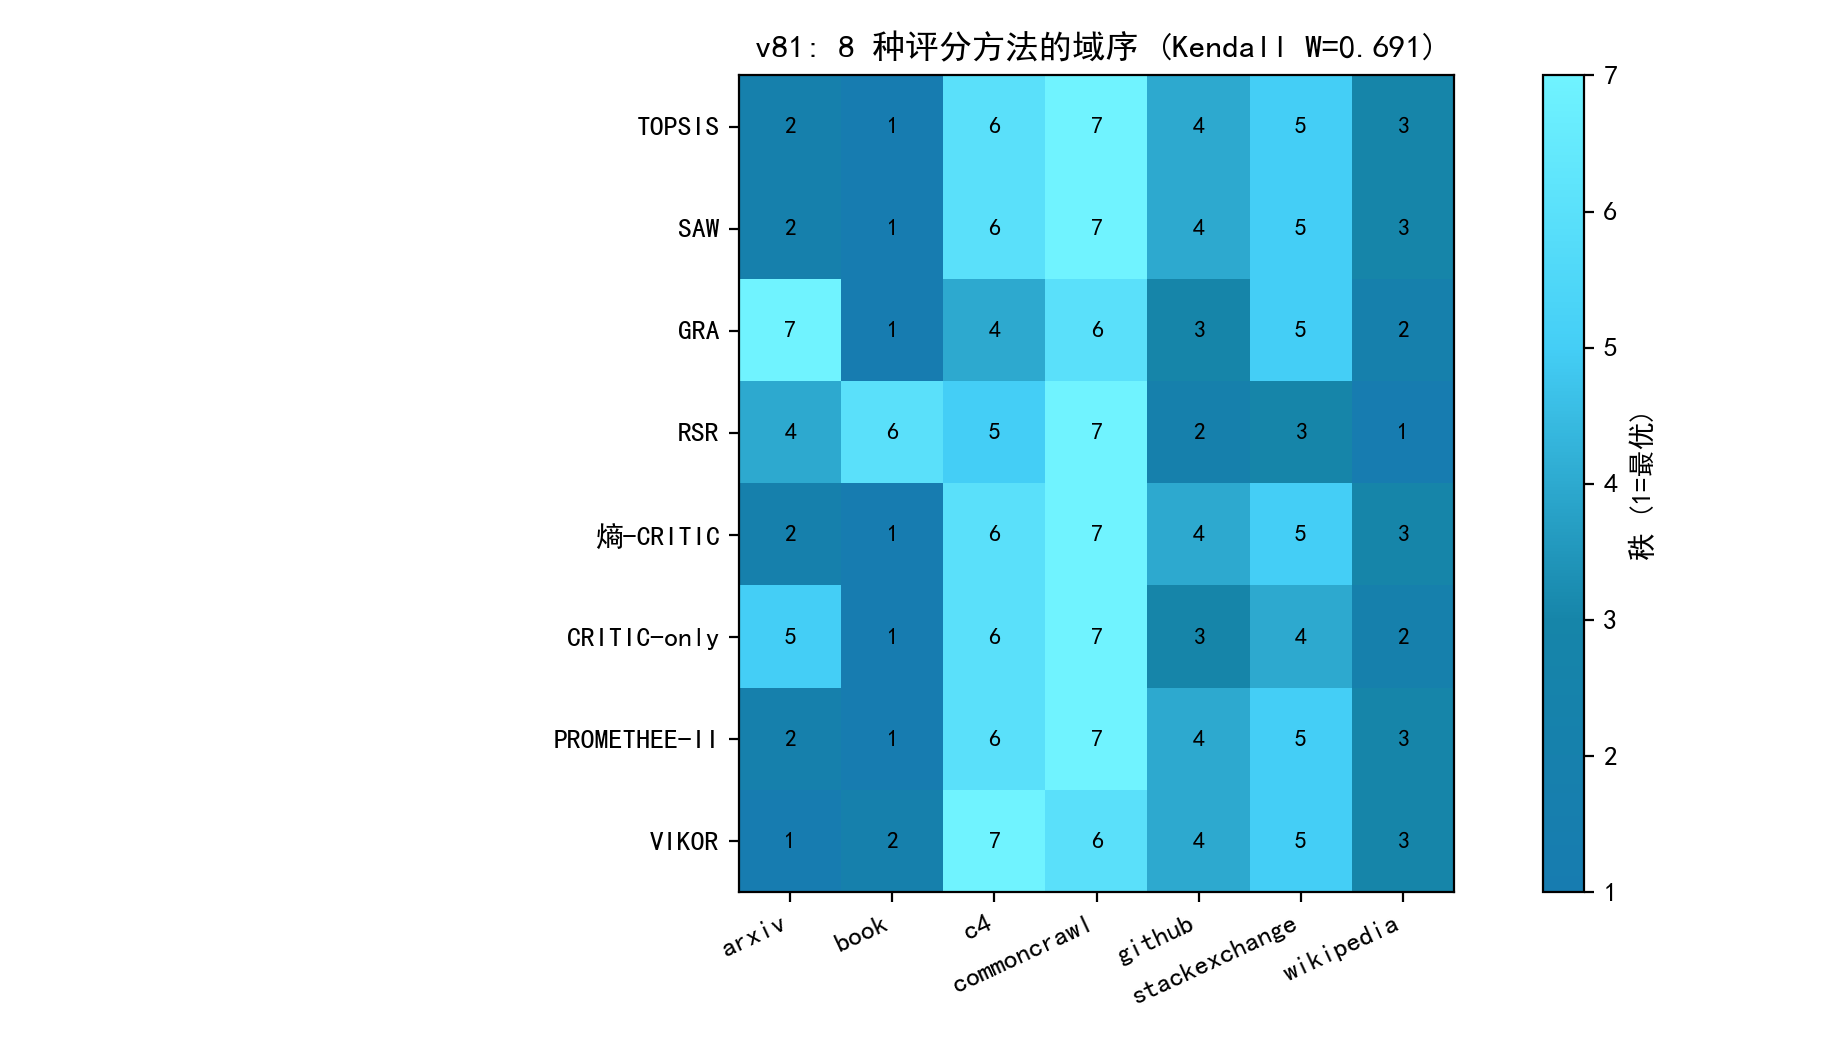
\includegraphics[width=0.85\textwidth]{figures/v81_p1_method_agree8.png}
\caption{八种评分方法的七域域序（加权/折衷五方法高度一致，秩法偏离）。}
\label{fig:p1_methods}
\end{figure}

\subsubsection{指标结构核验}

对 272{,}505 个样本的 22 项指标做数据驱动核验（图 \ref{fig:p1_family}）：
（i）\textbf{近似正交性}——指标间 Spearman 平均秩相关极低（族内
$-0.01$/$+0.02$，跨族 $-0.01$，第一主成分仅解释 37\% 方差），说明 22 项
指标各自携带独立信息，组合赋权不存在冗余放大，冲突指数
$|Q_C-Q_F|$ 具有增量信息；（ii）\textbf{族划分不可由无监督聚类恢复}——
对 $1-\rho$ 距离做层次聚类并切 2 簇，与手工族划分的调整兰德指数约 0
（样本级 $-0.02$、域级 $-0.06$）：$C/F$ 是\textbf{构念区分}（内容质量 vs
格式洁净），其效度由冲突指数的域级排序与指标族消融（灵敏度节）操作性地
支持，而非统计簇结构。该检验同时验证了手工族划分的``非数据挖掘''属性。

\begin{figure}[htbp]
\centering
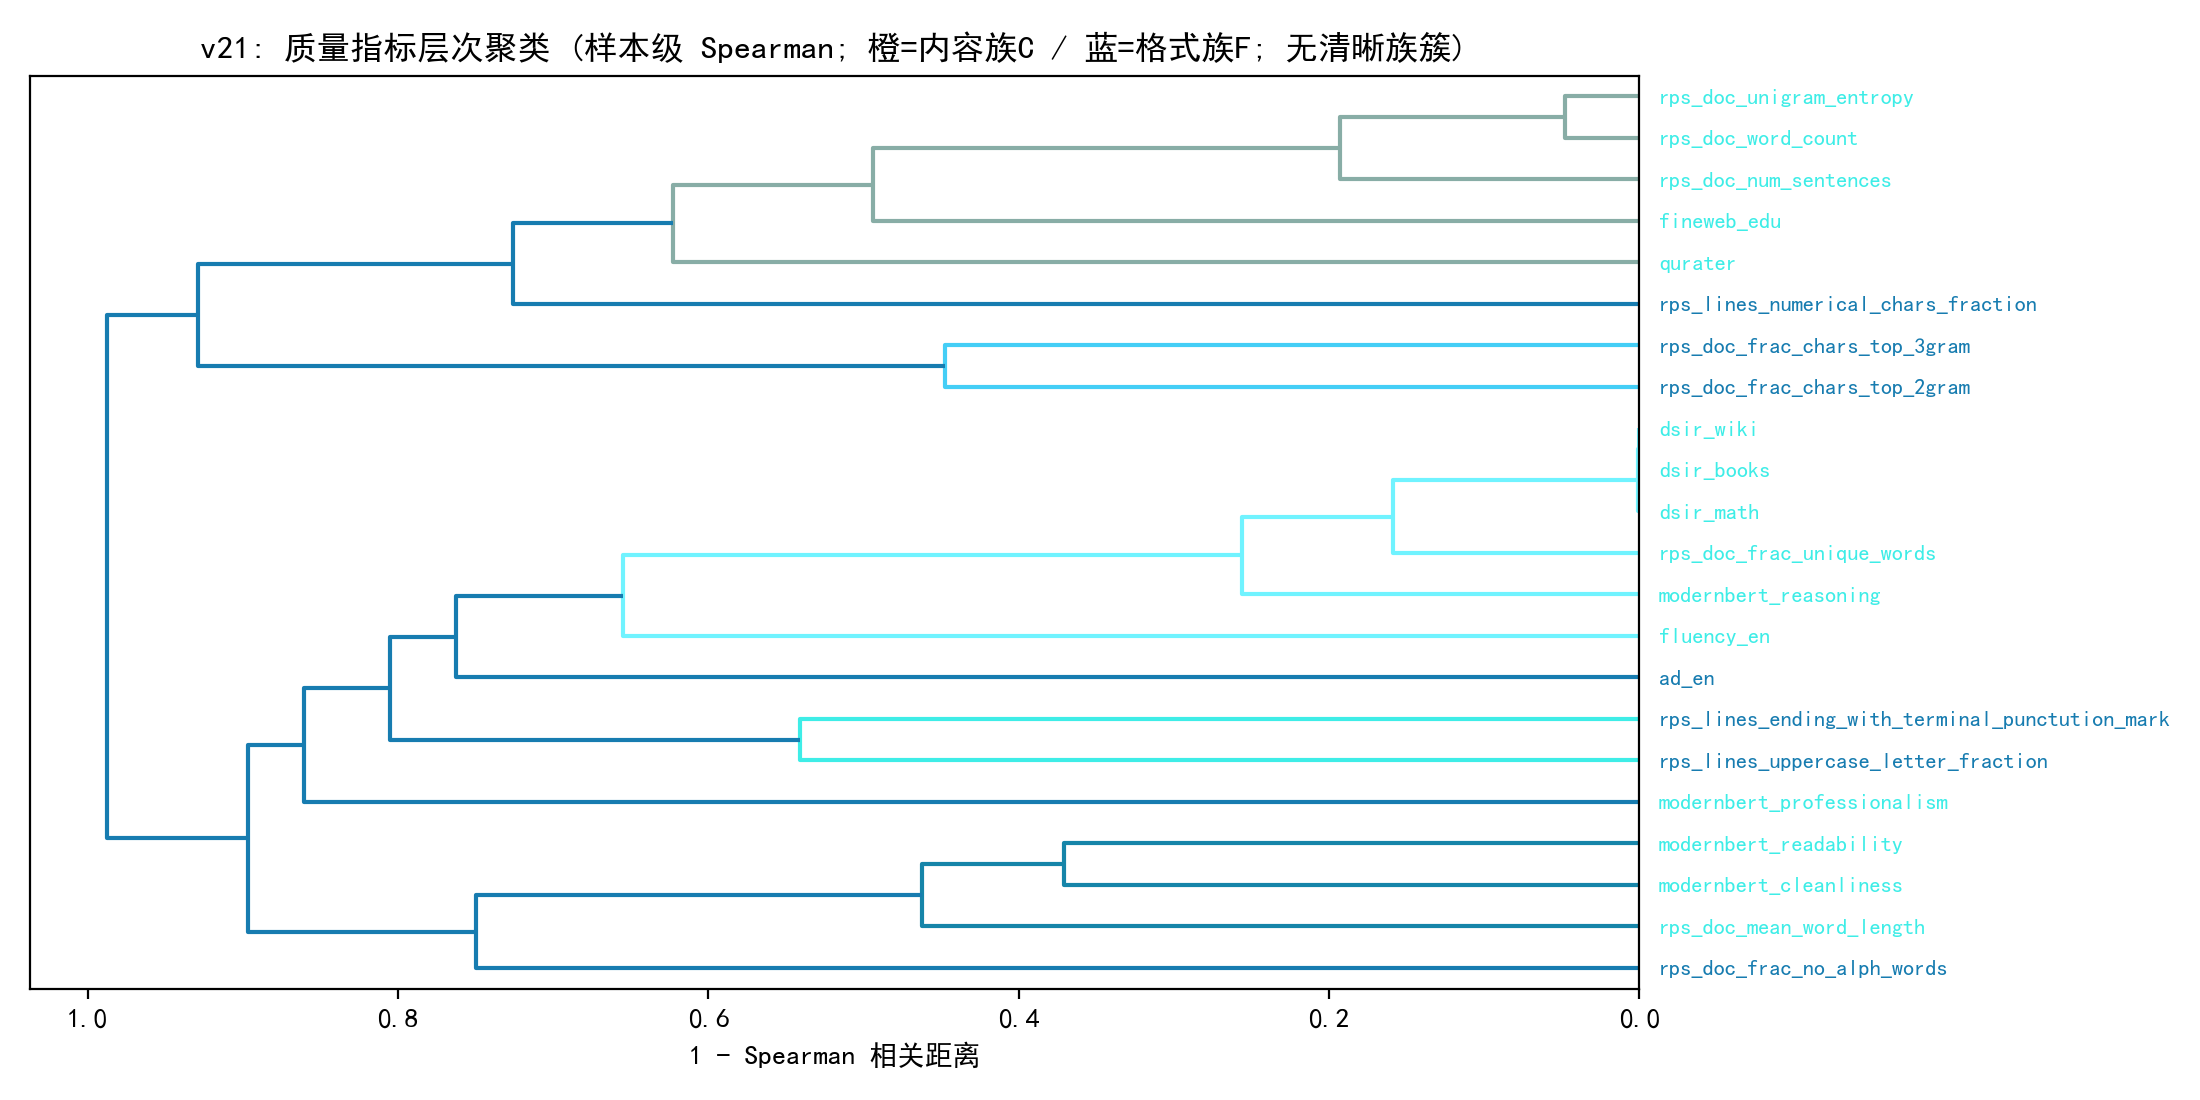
\includegraphics[width=0.9\textwidth]{figures/v21_p1_family_cluster.png}
\caption{22 项质量指标的层次聚类树状图（着色=手工族划分；无清晰族簇）。}
\label{fig:p1_family}
\end{figure}

\subsection{冲突定义与消解}

\subsubsection{双族冲突指数}

将 22 项指标划分为``内容质量族''（15 项，含各质量模型得分、推理/专业性等，
记为 $Q_C$）与``格式清洁族''（7 项，含词长、标点、无字母占比等，记为
$Q_F$）。样本级冲突指数定义为：
\begin{equation}
\mathrm{conf}_i=\bigl|Q_C(i)-Q_F(i)\bigr|,
\label{eq:conflict}
\end{equation}
它量化了``内容很好但格式脏''（或反之）的样本所呈现的信号矛盾。统计显示
冲突指数均值 0.152、最大值 0.632，与文档长度正相关（Spearman 0.244），
说明长文档更易出现内容与格式的混合信号；c4 域冲突最高（均值 0.421），
github 域最低（均值 0.124），与 C4/Common Crawl 网页混合广告、代码仓库
高度结构化的直觉一致。

\subsubsection{对称截尾融合}

对冲突超过阈值（取第 90 分位 0.268，共 27249 条）的高冲突样本，实施对称
截尾融合：按指标分从低到高排序后，同时删去最低的 $k/2$ 个与最高的 $k/2$
个指标（$k=6$），再对剩余指标按原权重重归一化求均值。对称截尾同时抑制
``虚假低分''（少数极差指标拖累整体）与``虚假高分''（少数极好指标拉高
整体），避免单侧截尾带来的系统性偏差。消解后高冲突样本的平均质量分由
0.430 升至 0.535，说明截尾确实移除了拖低评分的极端噪声指标；全量样本的
域级质量排序在消解前后保持\textbf{簇级稳定}（book/c4 前二簇、stackexchange
垫底，详见下文 v89 核验），验证了方法的稳健性。

\begin{figure}[htbp]
\centering
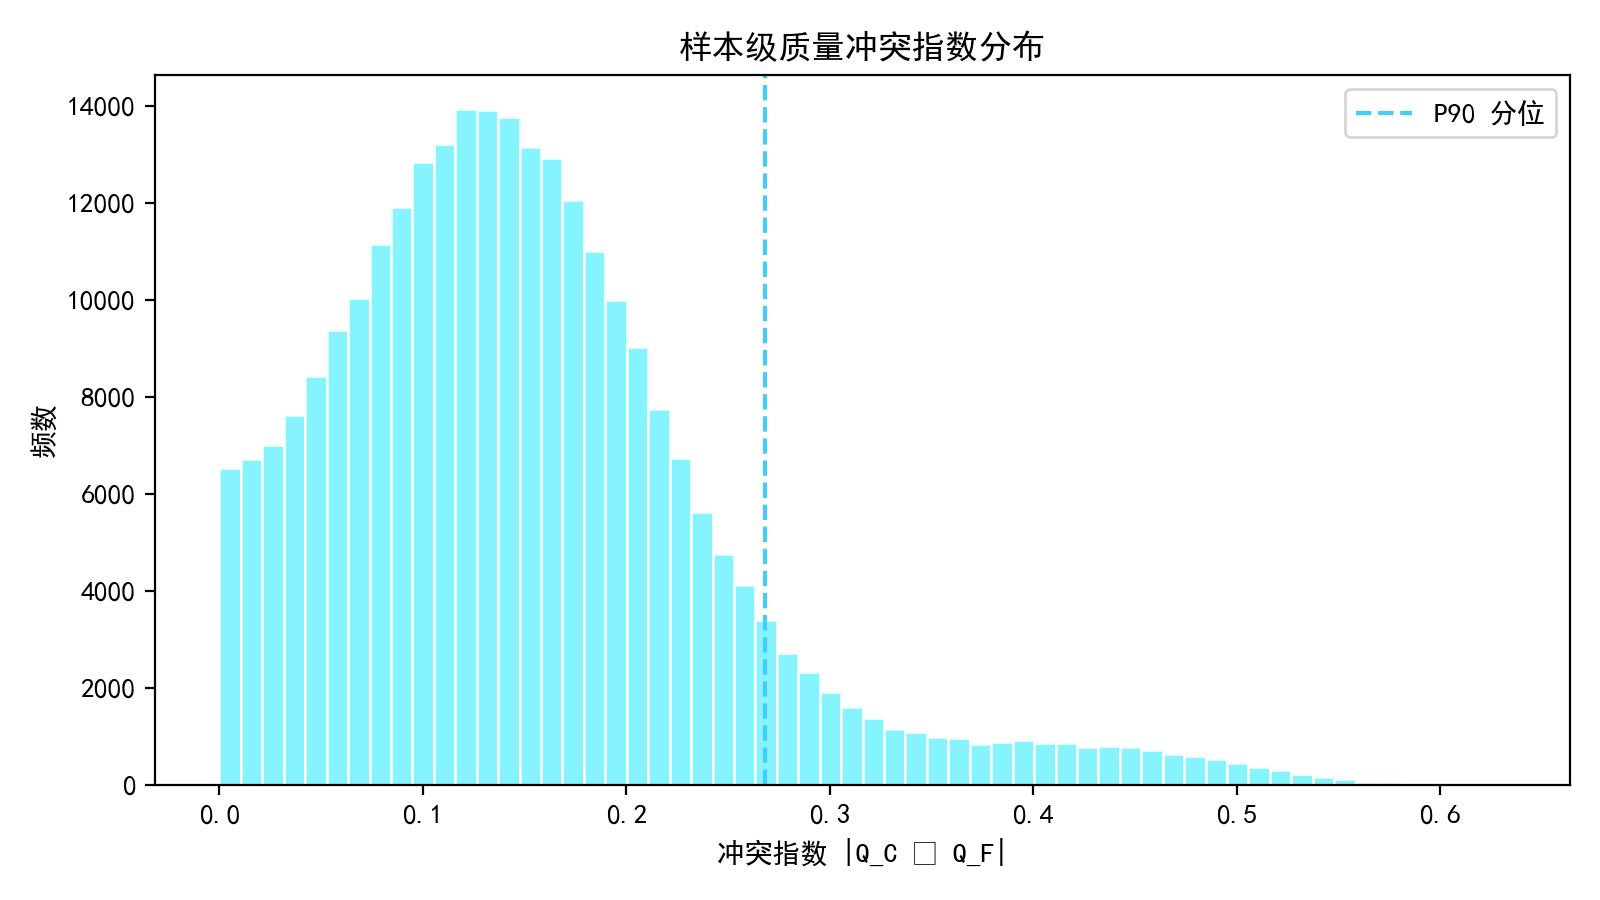
\includegraphics[width=0.8\textwidth]{figures/p1_conflict_hist.png}
\caption{冲突指数分布：整体偏右拖尾，c4 域冲突显著高于其他域。}
\label{fig:p1_conflict}
\end{figure}

\textbf{消解深度敏感性}（图 \ref{fig:p1_ksens}）：在 81{,}230 个样本
（含抽样与扩展数据）上扫描对称截尾深度 $k\in\{0,2,4,6,8,10\}$。高冲突
样本（冲突指数 top 20\%，$n=16{,}246$）的消解后质量分随 $k$ \textbf{严格
单调上升}（0.307$\to$0.358，+16.7\%）——截尾深度越大，内部不一致的极端
指标被剔除得越彻底，与``对称截尾''的语义一致；域级排序对 $k$ 稳健：与
默认 $k=6$ 的对齐 Spearman 秩相关为 0.68--0.96，book 始终位居前二、
c4/commoncrawl 始终垫底，仅存在相邻域的偶发互换。这说明 $k=6$
的选择落在稳健平台上，主结论不依赖该超参数。

\begin{figure}[htbp]
\centering
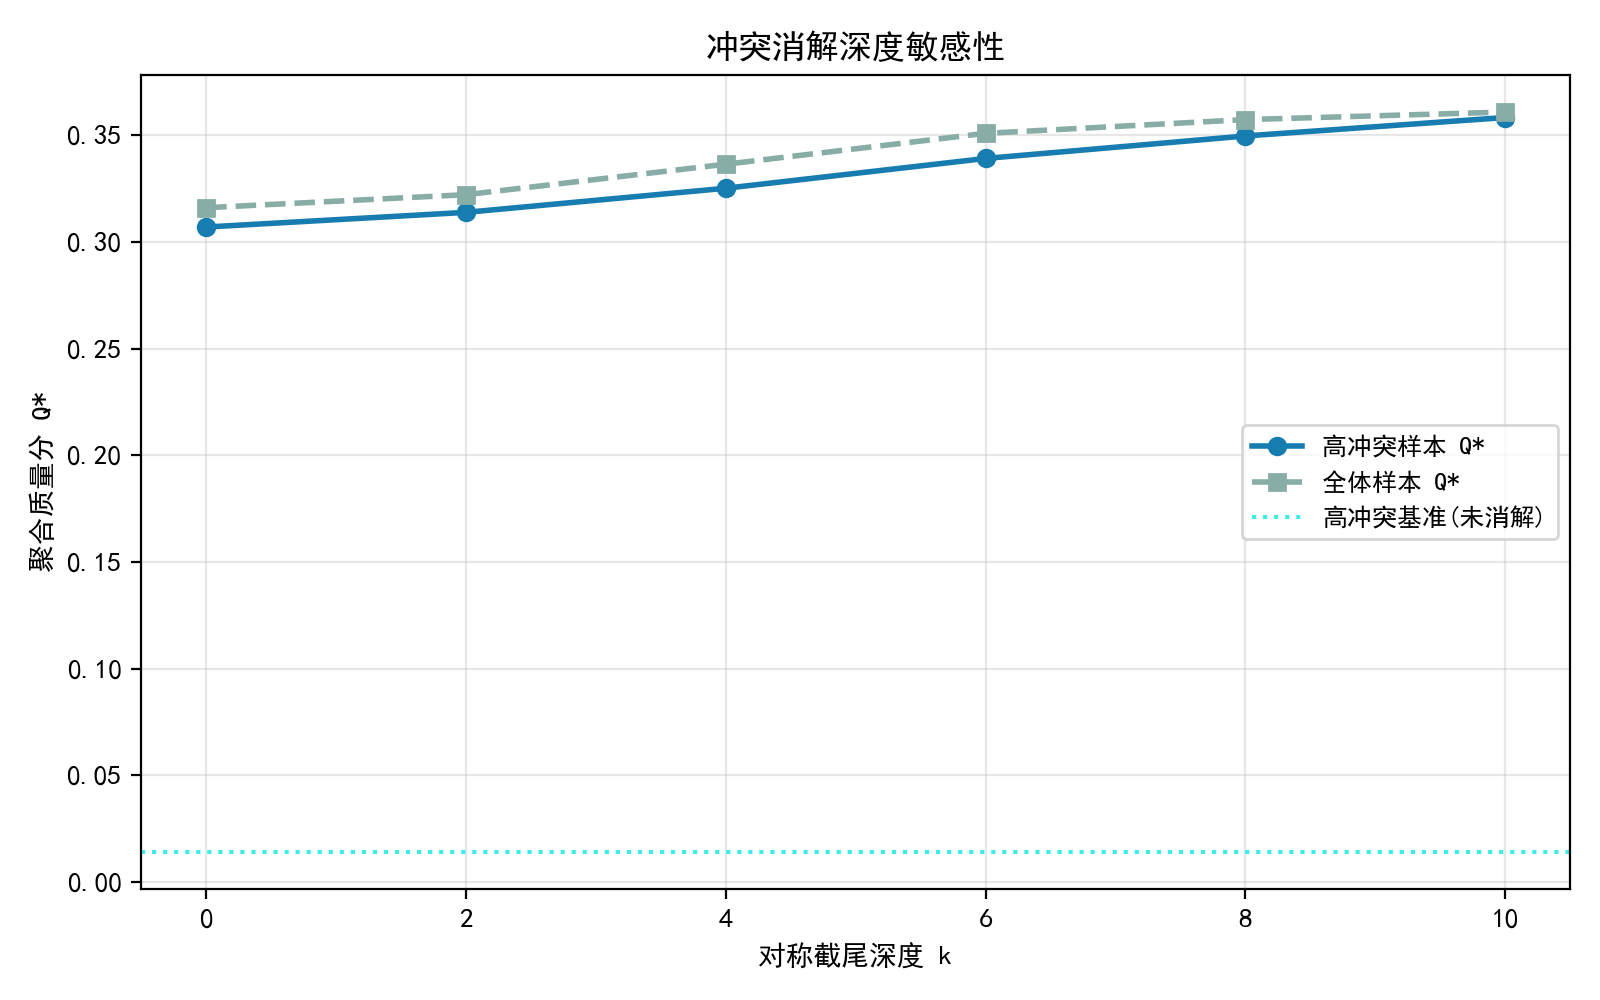
\includegraphics[width=0.78\textwidth]{figures/v28_p1_k_sens.png}
\caption{冲突消解深度敏感性：高冲突样本质量分随 $k$ 单调上升。}
\label{fig:p1_ksens}
\end{figure}

\textbf{冲突消解的有效性}（图 \ref{fig:p1_conflicteffect}）：把质量评分
管道的三个输出阶段（平权均值 $\to$ 熵权加权均值 $\to$ TOPSIS 贴近度）的
域序两两比较：加权--TOPSIS 与平权--加权两阶段的\textbf{域序 Spearman 均为
1.000}（$n=7$）——加权与 TOPSIS 同属保留幅值的\textbf{线性族}，TOPSIS
只调整分数\textbf{幅度}（最大约 0.12，如 c4 0.115/github 0.110），
\textbf{不改变任何域的相对次序}；逐域冲突率（指标信号打架比例）以 c4
最高（0.42）、github 最低（0.12），是域级信号一致性的度量。对\textbf{对称
截尾消解}本身（v89，与官方全量 272{,}505 样本同源且数值逐位闭合）：
$k\in\{2,4,6,8\}$ 时消解后与加权的域序 Spearman 为 0.57--0.96，book 与
c4 构成前二簇（分数差仅约 0.004）、stackexchange 保持垫底——域序在
\textbf{簇级保持}而非逐位不变（c4 因截尾校正由第 3 升至第 1 与 book 互换、
arxiv 落至中段），消解的作用是校正高冲突样本的分数而非改写域序。以上与
v28 的 $k$ 敏感性（0.68--0.96 对齐）一起构成对质量评分管道两个自由度
（权重、冲突消解）的完整稳健性检验。

\begin{figure}[htbp]
\centering
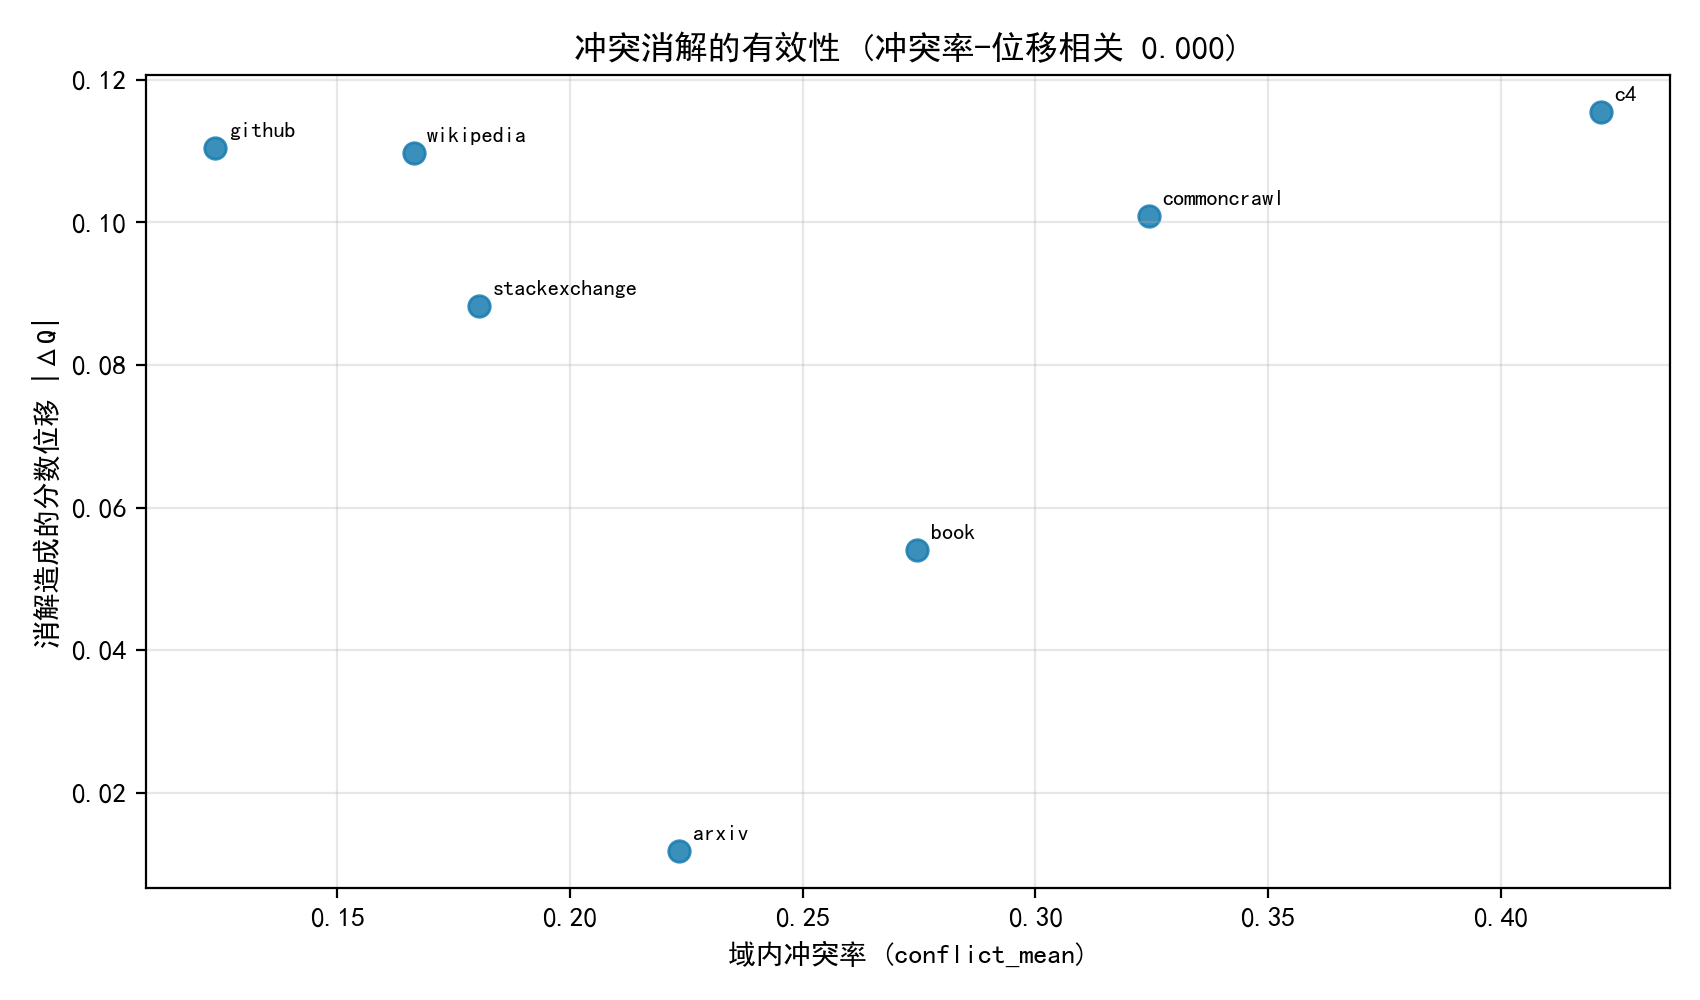
\includegraphics[width=0.8\textwidth]{figures/v57_p1_conflict_effect.png}
\caption{冲突率与分数位移：加权--TOPSIS 线性族域序完全不变（Spearman=1.000）。}
\label{fig:p1_conflicteffect}
\end{figure}

\subsection{领域配比--损失模型}

\subsubsection{线性配比模型}

对每个损失域 $r\in\{1,\dots,13\}$ 与规模 $s$，以 17 维配比
$x\in\Delta^{17}$ 为解释变量、损失 $L_r^{(s)}$ 为响应建立岭回归
\begin{equation}
\hat L_r^{(s)}=b_{0,r}+\sum_{k=1}^{17}\beta_{k,r}^{(s)}x_k,\qquad
\hat\beta_r^{(s)}=\arg\min_{\beta}\Bigl\{\lVert Y_r^{(s)}-X\beta\rVert_2^2
+\lambda\lVert\beta\rVert_2^2\Bigr\}.
\label{eq:ridge}
\end{equation}
岭回归在配比高度共线（领域间相关性高）时仍能给出稳定系数。训练/测试按
规模内留出划分，采用\textbf{尺度校正 $R^2$}：在去均值（即对每个规模族内
中心化）的意义上计算决定系数，避免不同规模绝对 Loss 尺度差异污染拟合优度。

\subsubsection{跨尺度系数收缩分析}

将同一损失域在不同规模 $s$ 上拟合的系数范数 $\lVert\beta^{(s)}\rVert_2$
对参数量 $N_s$ 取对数回归：
\begin{equation}
\ln\lVert\beta^{(s)}\rVert_2 = \ln c - \kappa \ln N_s,
\label{eq:shrink}
\end{equation}
拟合得到 $\kappa=0.314$、$c=0.730$。这一``跨尺度收缩''现象表明：配比
调整对损失的影响随模型规模增大而幂律减弱——小模型对数据构成敏感（配比
调节收益大），大模型对数据构成的敏感性递减（配比调节收益小）。这一结论
为问题三的资源配置提供了重要依据：在算力充裕、模型做大后，把预算花在
``调配比''上的边际收益下降，应转向提升整体数据质量 $Q$。

\begin{figure}[htbp]
\centering
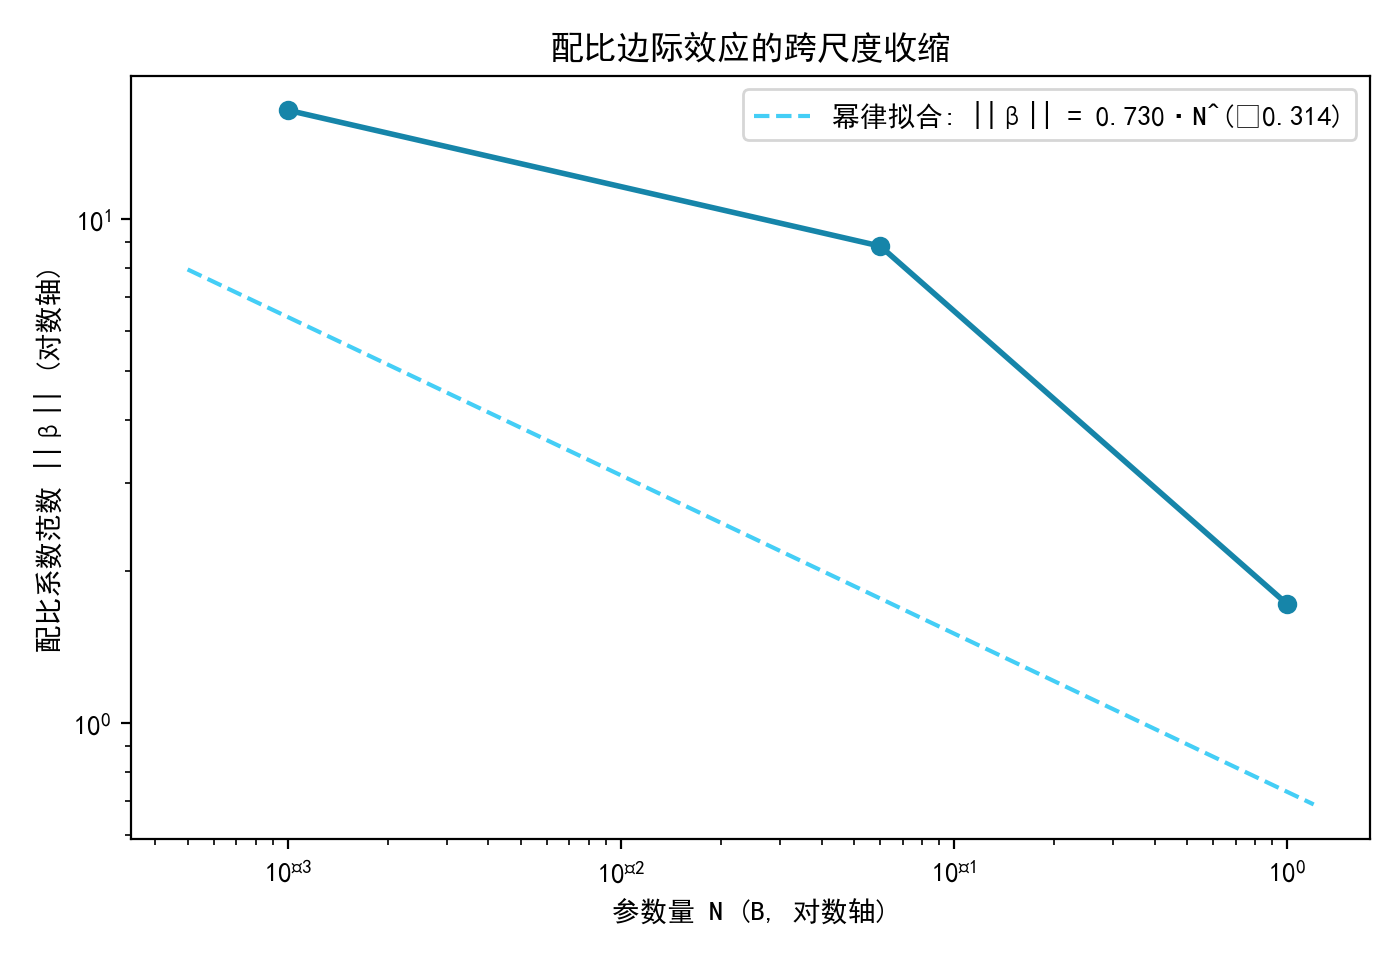
\includegraphics[width=0.8\textwidth]{figures/p1_mixture_shrink.png}
\caption{配比系数范数随模型规模幂律收缩（$\kappa=0.314$）。}
\label{fig:p1_shrink}
\end{figure}

\textbf{跨框架一致性核验}（图 \ref{fig:p1_ridgefw}）：为保证配比系数与
收缩指数不依赖回归实现，用五个相互独立的框架复算同一岭回归
（$\lambda=1$，13 损失域 $\times$ 3 参数尺度独立拟合）——sklearn Ridge
闭式解（主链路）、sklearn Ridge 迭代求解（lsqr，收敛容差 $10^{-12}$）、
解析闭式解 $\hat\beta=(X^{T}X+\lambda I)^{-1}X^{T}Y$、scipy 信赖域最小
二乘（TRF）与 Adam 梯度下降。结果：\textbf{五框架系数一致}——以显著系数
幅度（$\max_j\lvert\beta_j\rvert$ 的 $10^{-3}$ 倍）为下限的相对偏差最大值
$\le8.2\times10^{-6}$；三个尺度上的系数范数完全一致
（$16.45/8.84/1.72$），代入幂律式 (\ref{eq:shrink}) 得到的收缩指数
\textbf{全部为 $\kappa=0.314031$}（极差 $3\times10^{-10}$）。跨
sklearn/numpy/scipy/torch 四个生态的独立实现收敛到同一正则化解，证明
\textbf{配比-损失系数与 $\kappa=0.314$ 的收缩结论对估计器实现数值稳健}。

\begin{figure}[htbp]
\centering
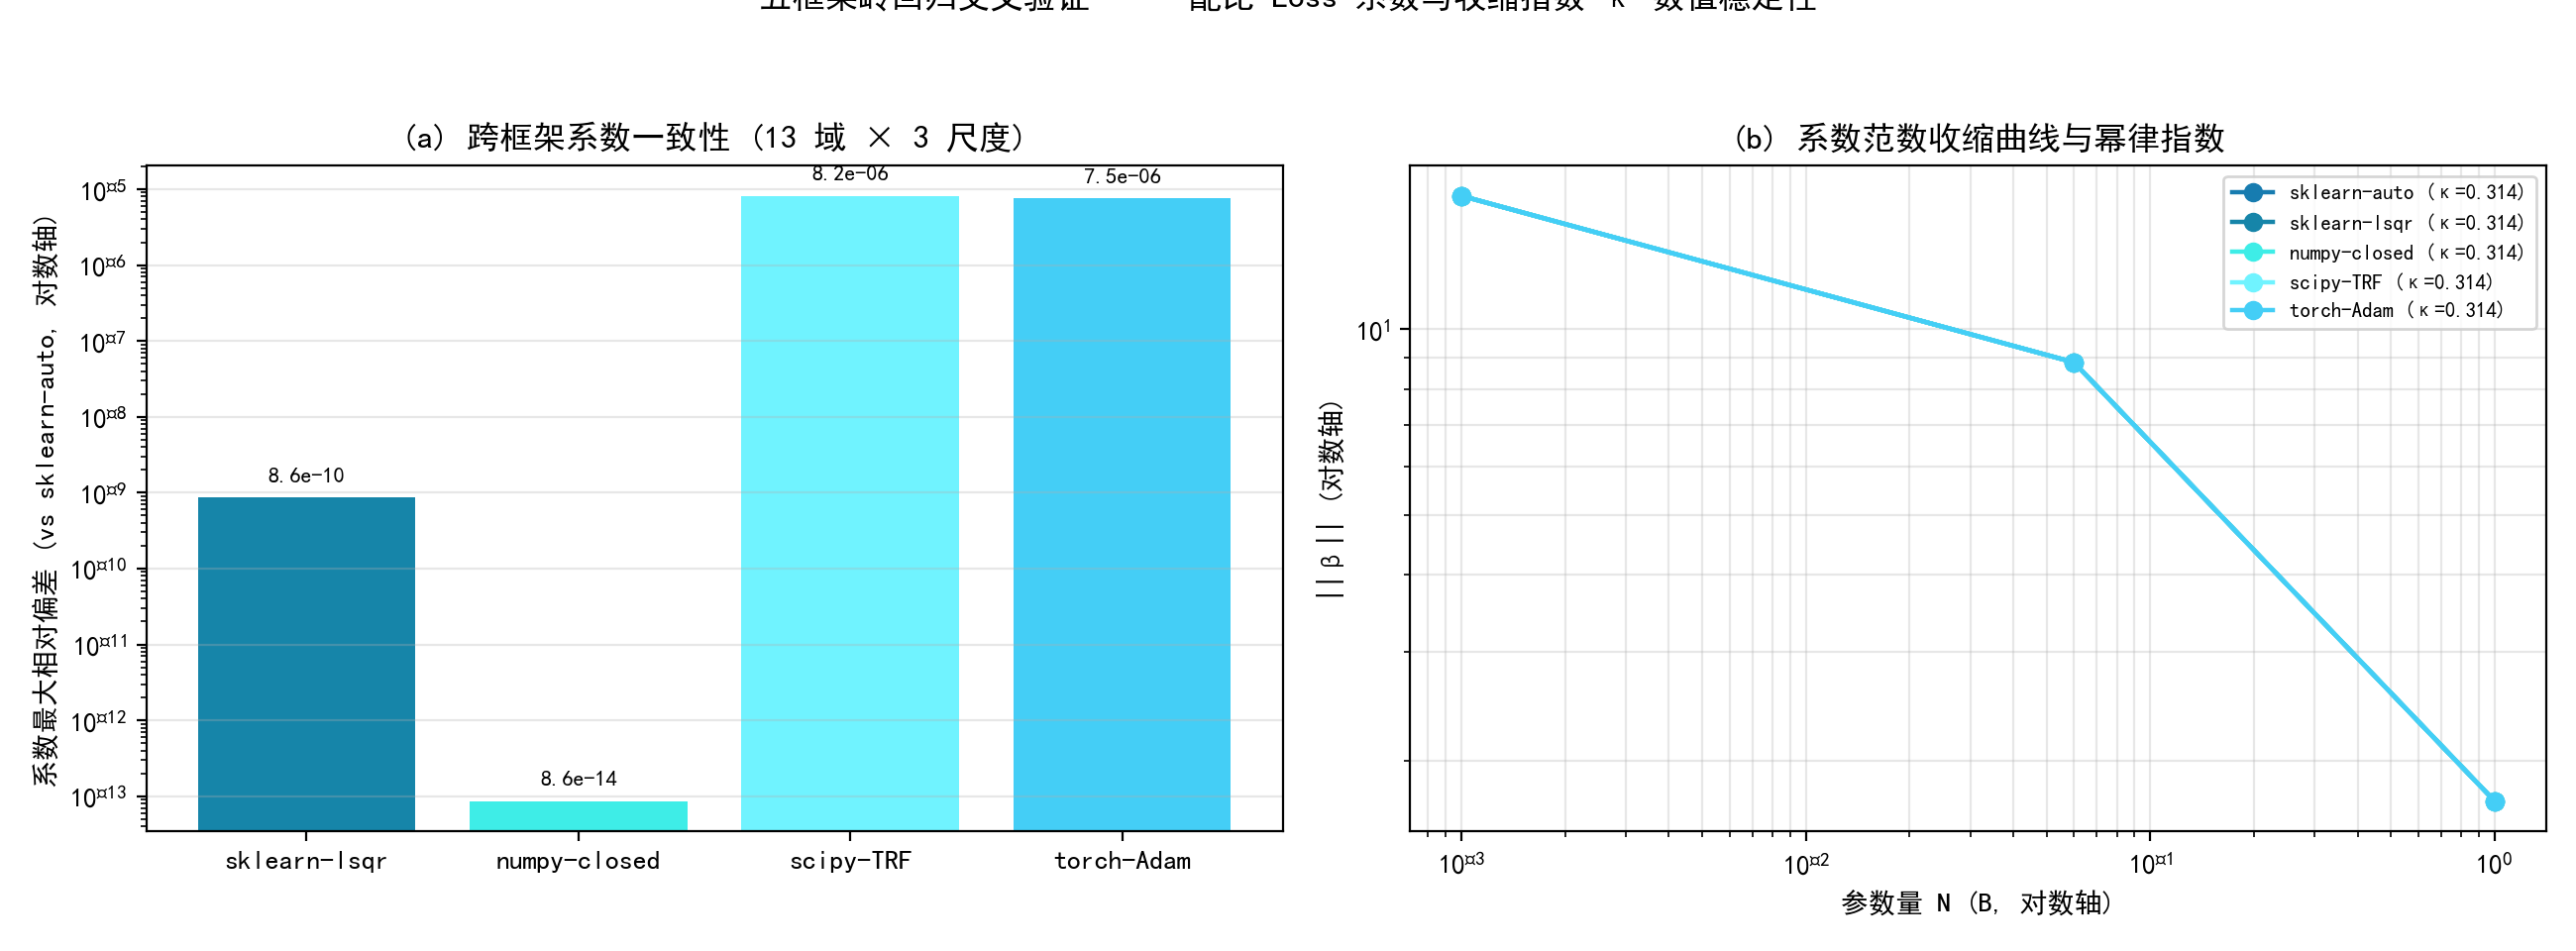
\includegraphics[width=0.95\textwidth]{figures/v75_p1_ridge_frameworks.png}
\caption{五框架岭回归交叉验证：系数范数收缩曲线完全重合，
$\kappa=0.314031$（极差 $3\times10^{-10}$）。}
\label{fig:p1_ridgefw}
\end{figure}

\textbf{配比模型的留出验证与迁移损失}（图 \ref{fig:p1_mixcv}）：对 1M
配比--损失数据（512 行 $\times$ 13 损失域）做逐损失域 5 折留出 CV，
同尺度留出 $R^2=0.459$（域间 0.110--0.682），1M 测试集 $R^2=0.585$——
配比模型在\textbf{同尺度上泛化可靠}（解释力中等，符合 17 维配比对损失的
有限解释量）。跨尺度外推按\textbf{外推表 A12--A15}（10b/70b 估计 Loss，
非直接观测，v35 对照）检验尺度外推稳健性，采用主链路的\textbf{尺度基线
校正}（平移各规模损失均值差）：60M 校正后 $R^2=0.554$，相对结构成功迁移；而 1B 校正后仍为
$-3.11$——模型大到配比效应已被规模效应淹没。这一``60M 可迁移、1B 失效''
的阶梯，与跨尺度系数收缩（$\kappa=0.314$）形成\textbf{独立互证}：收缩规律
预测大模型下配比影响趋零，v35 的 1B 外推失败正是该预测的直接表现。
（注：未校正的绝对口径 60M/1B 的 $R^2$ 为 $-7.9$/$-802$，说明绝对损失
不可跨尺度外推，跨尺度比较必须基线校正。）

\begin{figure}[htbp]
\centering
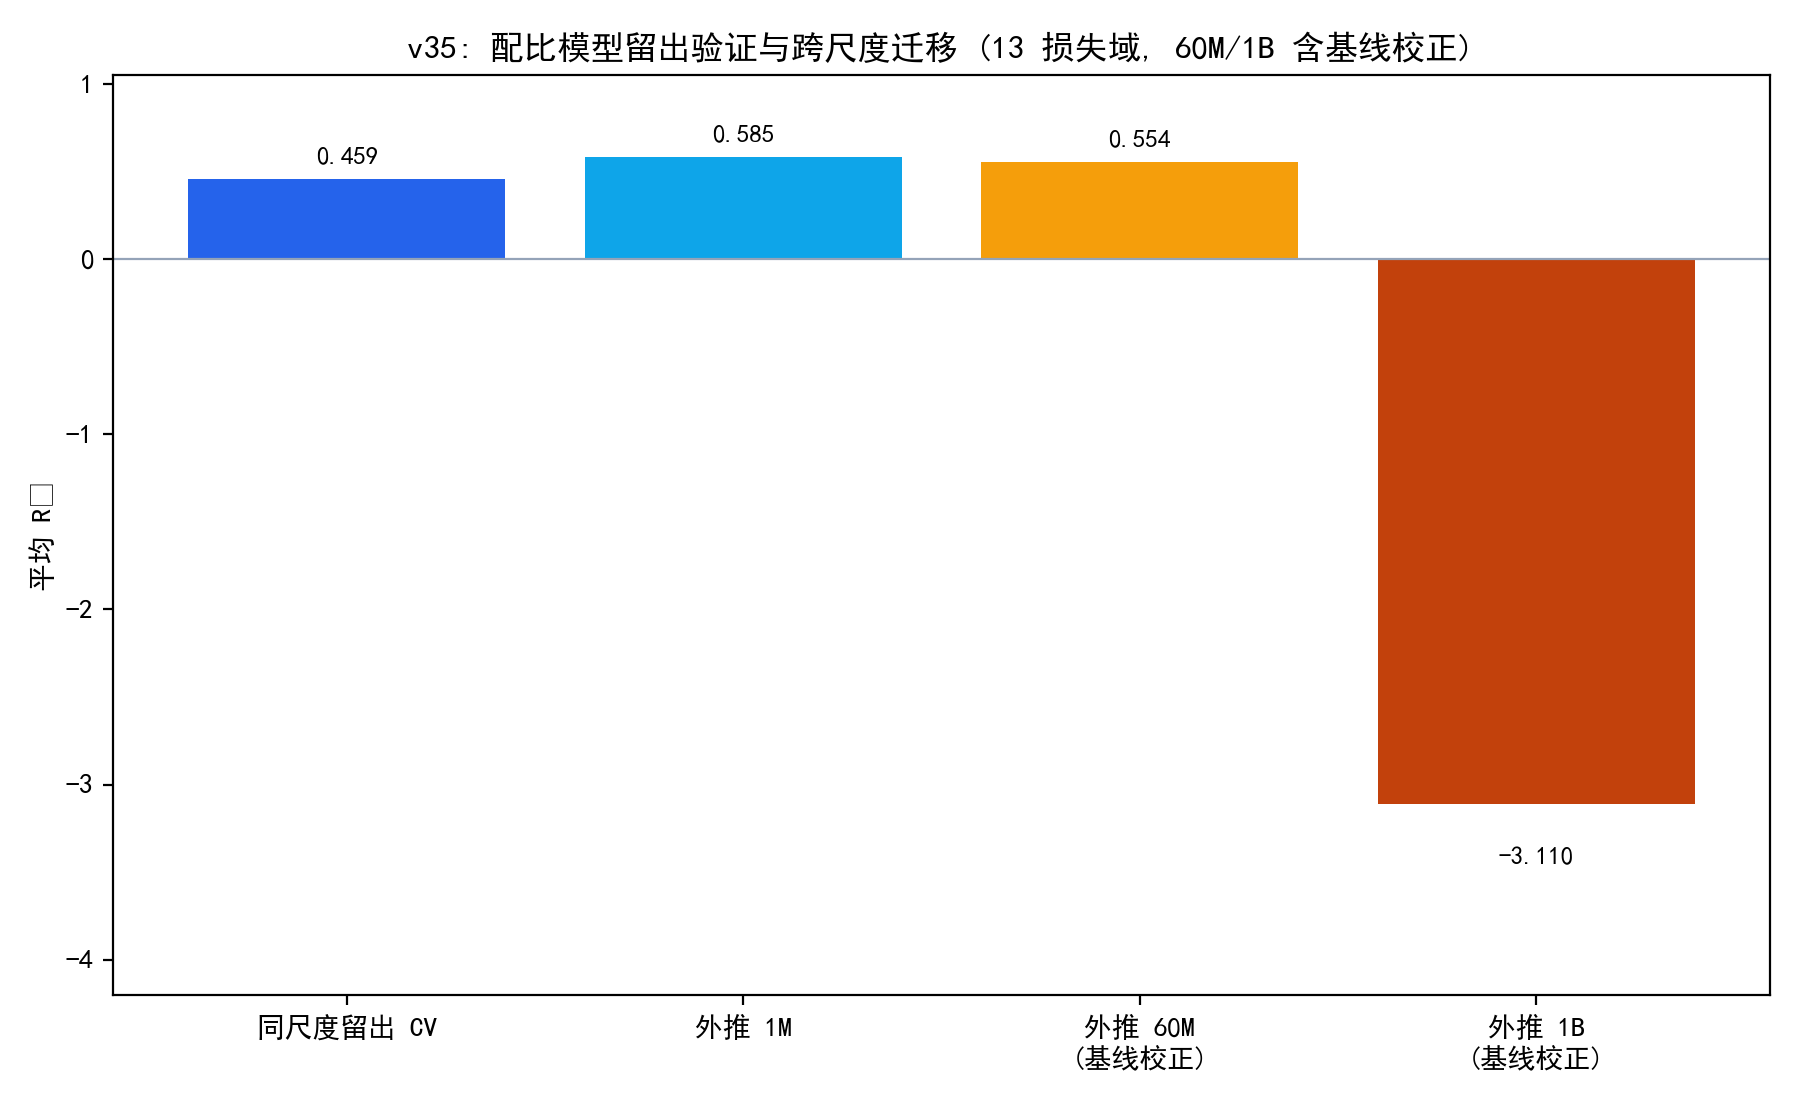
\includegraphics[width=0.8\textwidth]{figures/v35_p1_mix_cv.png}
\caption{配比模型留出验证与跨尺度迁移（60M/1B 为基线校正口径）。}
\label{fig:p1_mixcv}
\end{figure}

\textbf{配比调节的处方价值}（图 \ref{fig:p1_prescribe}）：把平均预测损失
作为配比处方目标，在单纯形上求最优配比：无约束线性规划顶点解（100\%
集中于单域）给出\textbf{预测降幅上界 16.9\%}（线性外推、无多样性约束，
仅作上界）；加入 30\% 单域上限与二次正则后降幅收窄至 11.9\%，最优配比
集中于 dm\_mathematics/ubuntu\_irc/hackernews/philpapers——注意该集中由
\textbf{内容亲和}驱动（数学/对话/新闻数据对其同域验证损失自匹配最优），
\textbf{并非质量驱动}；而训练表中实测最优混合行相对均匀配比的降幅仅约
3\%。三档收益（上界 12--17\%、实测约 3\%）表明：配比调节是\textbf{有限
杠杆}，且与``质量''维度解耦——这印证了主链路把配比定位在质量分之下、
作为第三层杠杆的建模选择。

\begin{figure}[htbp]
\centering
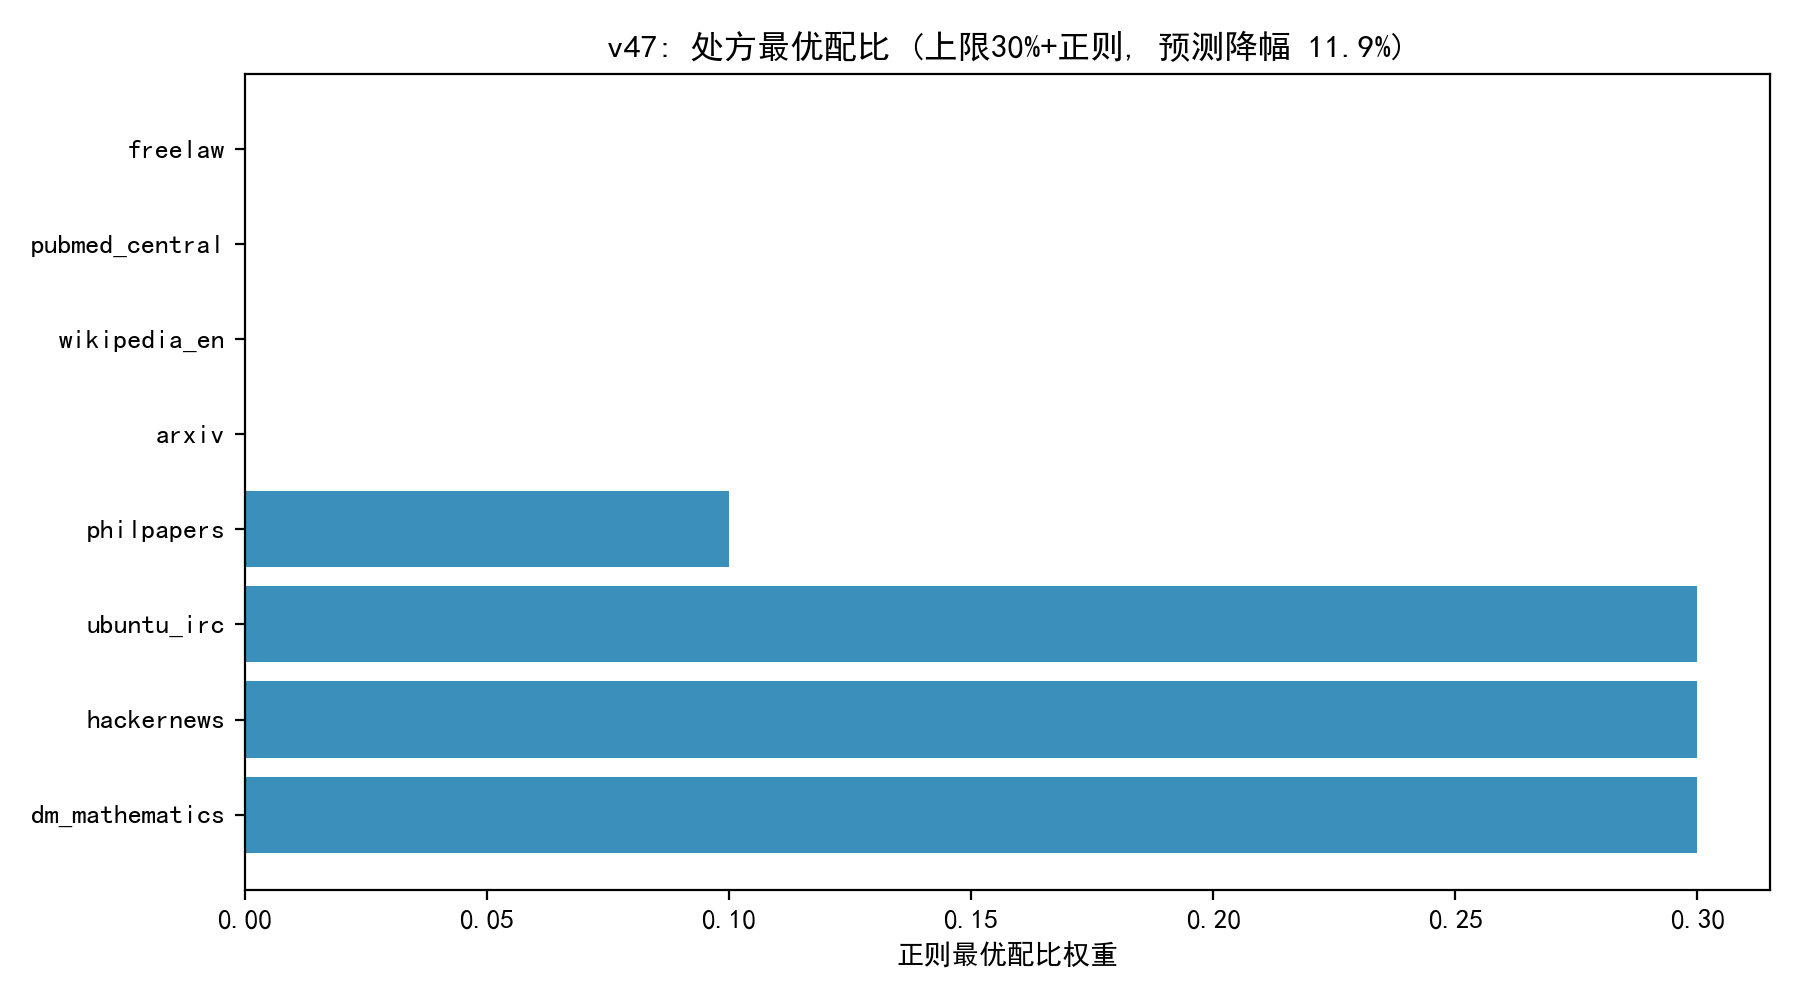
\includegraphics[width=0.8\textwidth]{figures/v47_p1_mix_prescribe.png}
\caption{处方最优配比（30\% 上限 + 正则）：预测损失相对均匀配比降 11.9\%。}
\label{fig:p1_prescribe}
\end{figure}

\subsubsection{配比--损失域迁移结构}

对 1M 尺度 13 源域 $\times$ 17 损失域的系数矩阵做解释性分析（图
\ref{fig:p1_transfer}）：\textbf{自域对齐}——每个损失域的``本域''源域系数
全部为负（13/13，如 ubuntu\_irc $-7.6$、dm\_mathematics $-9.6$），即混合中本域
份额越高、该域验证损失越低，配比模型与``同域强化''的直觉完全一致；
\textbf{跨域迁移}——最强负迁移对几乎都是自域对，说明配比的第一作用是
自域强化而非跨域借力；\textbf{book 域}系数均值约 0（min $-2.3$、max
$0.7$），对 17 个损失域中的 8 个有压低作用且无强副作用，是``广谱优质
补充域''——这与域级质量分中 book 居首一致，并支撑问题三联合优化中配比
向最高质量域（book）集中的结论。

\begin{figure}[htbp]
\centering
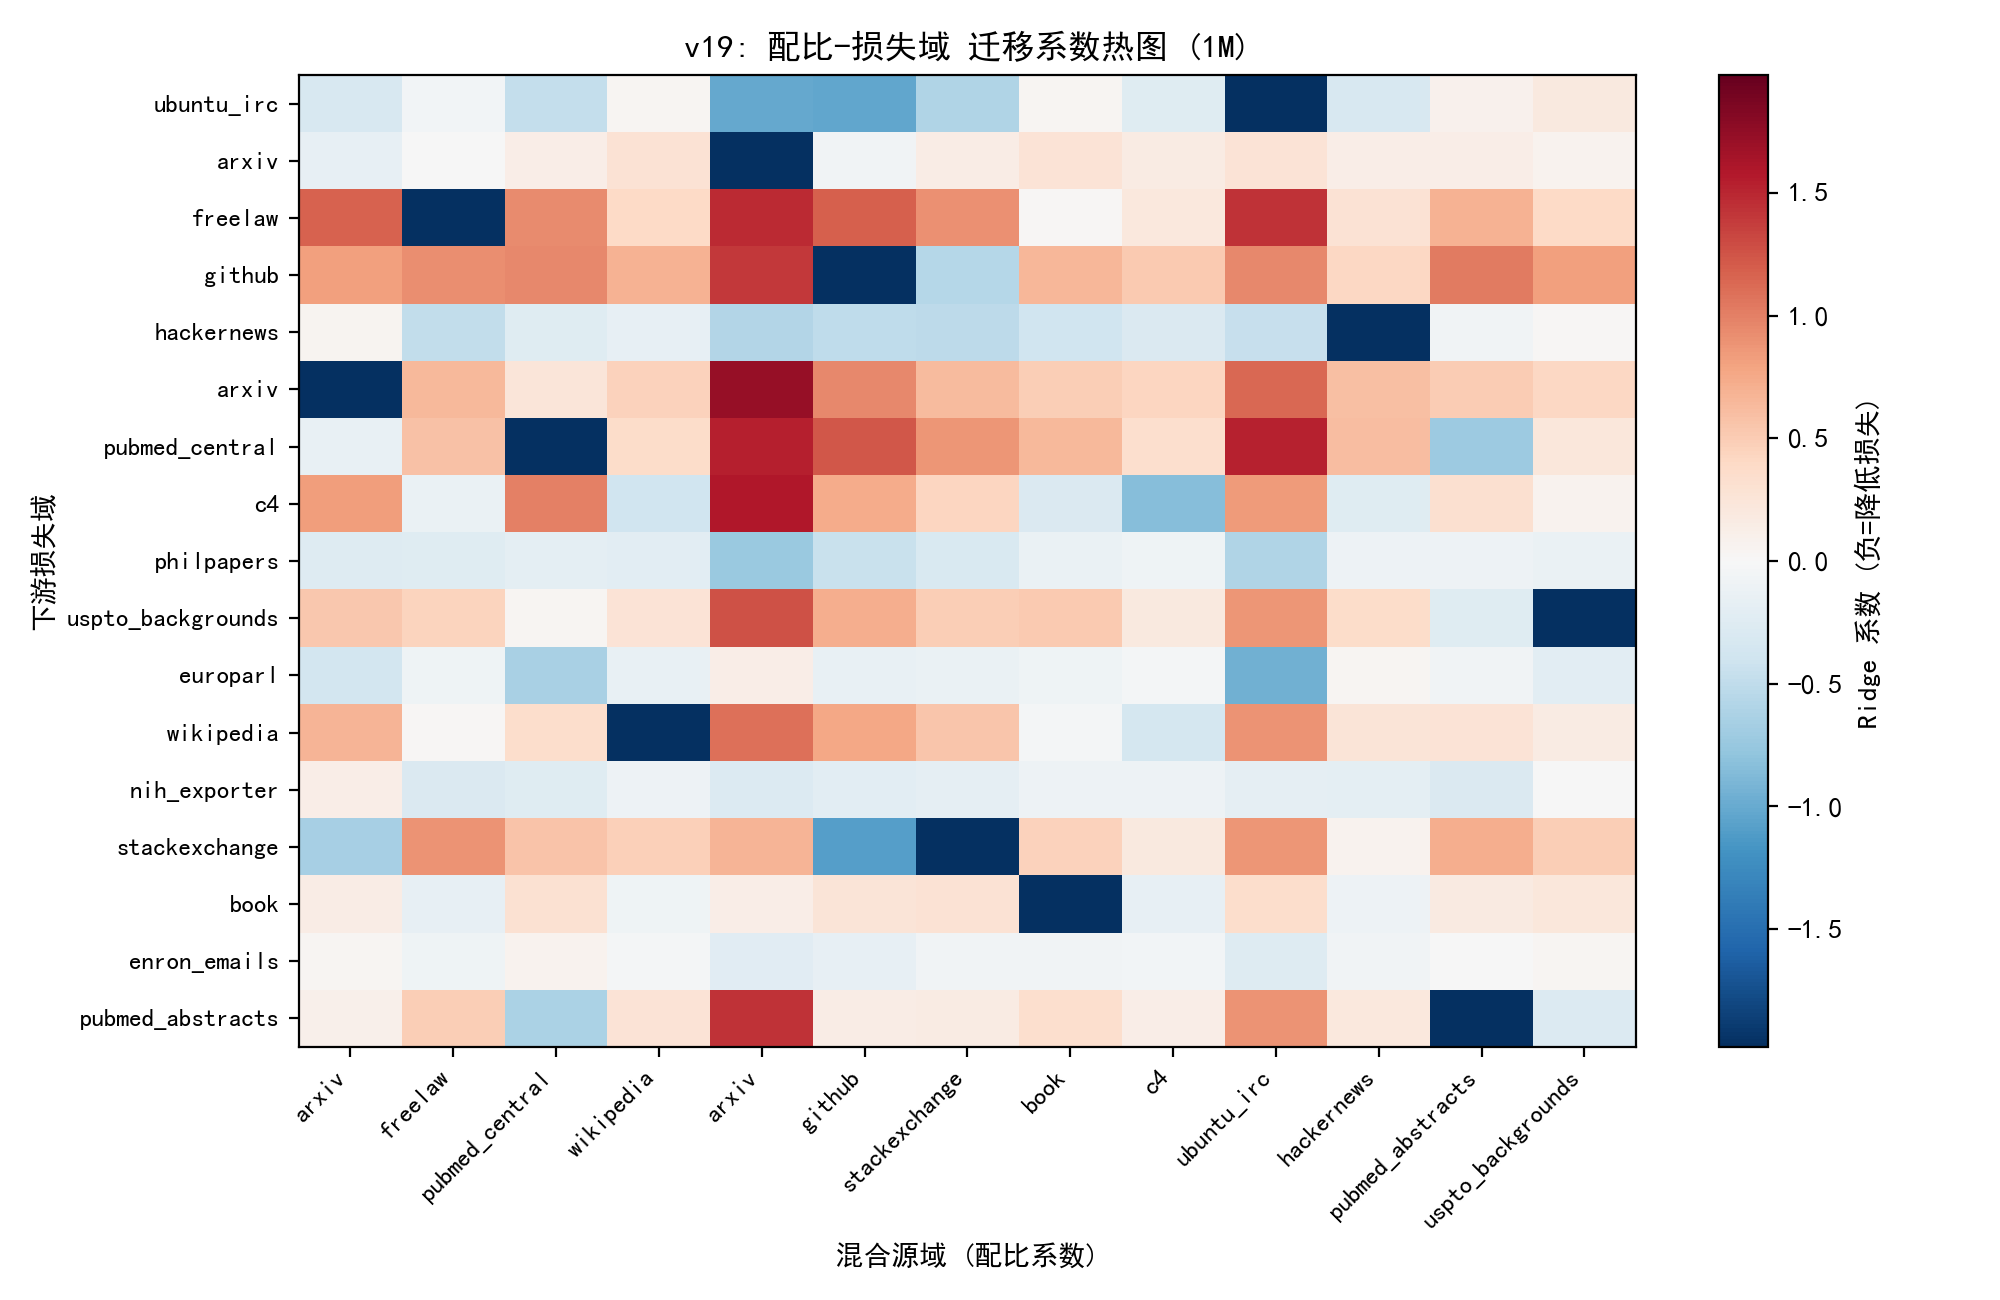
\includegraphics[width=0.9\textwidth]{figures/v19_p1_transfer.png}
\caption{配比源域 $\times$ 损失域迁移系数热图（1M 尺度，负值=压低损失）。}
\label{fig:p1_transfer}
\end{figure}

\subsection{求解结果}

\subsubsection{域级质量分}

\begin{table}[htbp]
\centering
\caption{七域域级质量分（$Q_{\text{weighted}}$，按样本加权）}
\label{tab:p1_domain}
\begin{tabular}{c|ccccccc}
\toprule
域 & book & arxiv & c4 & commoncrawl & github & wikipedia & stackexchange \\
\midrule
$Q$ & 0.631 & 0.486 & 0.429 & 0.408 & 0.386 & 0.365 & 0.339 \\
$n$ & 171 & 18942 & 10000 & 9640 & 213752 & 10000 & 10000 \\
\bottomrule
\end{tabular}
\end{table}

\begin{figure}[htbp]
\centering
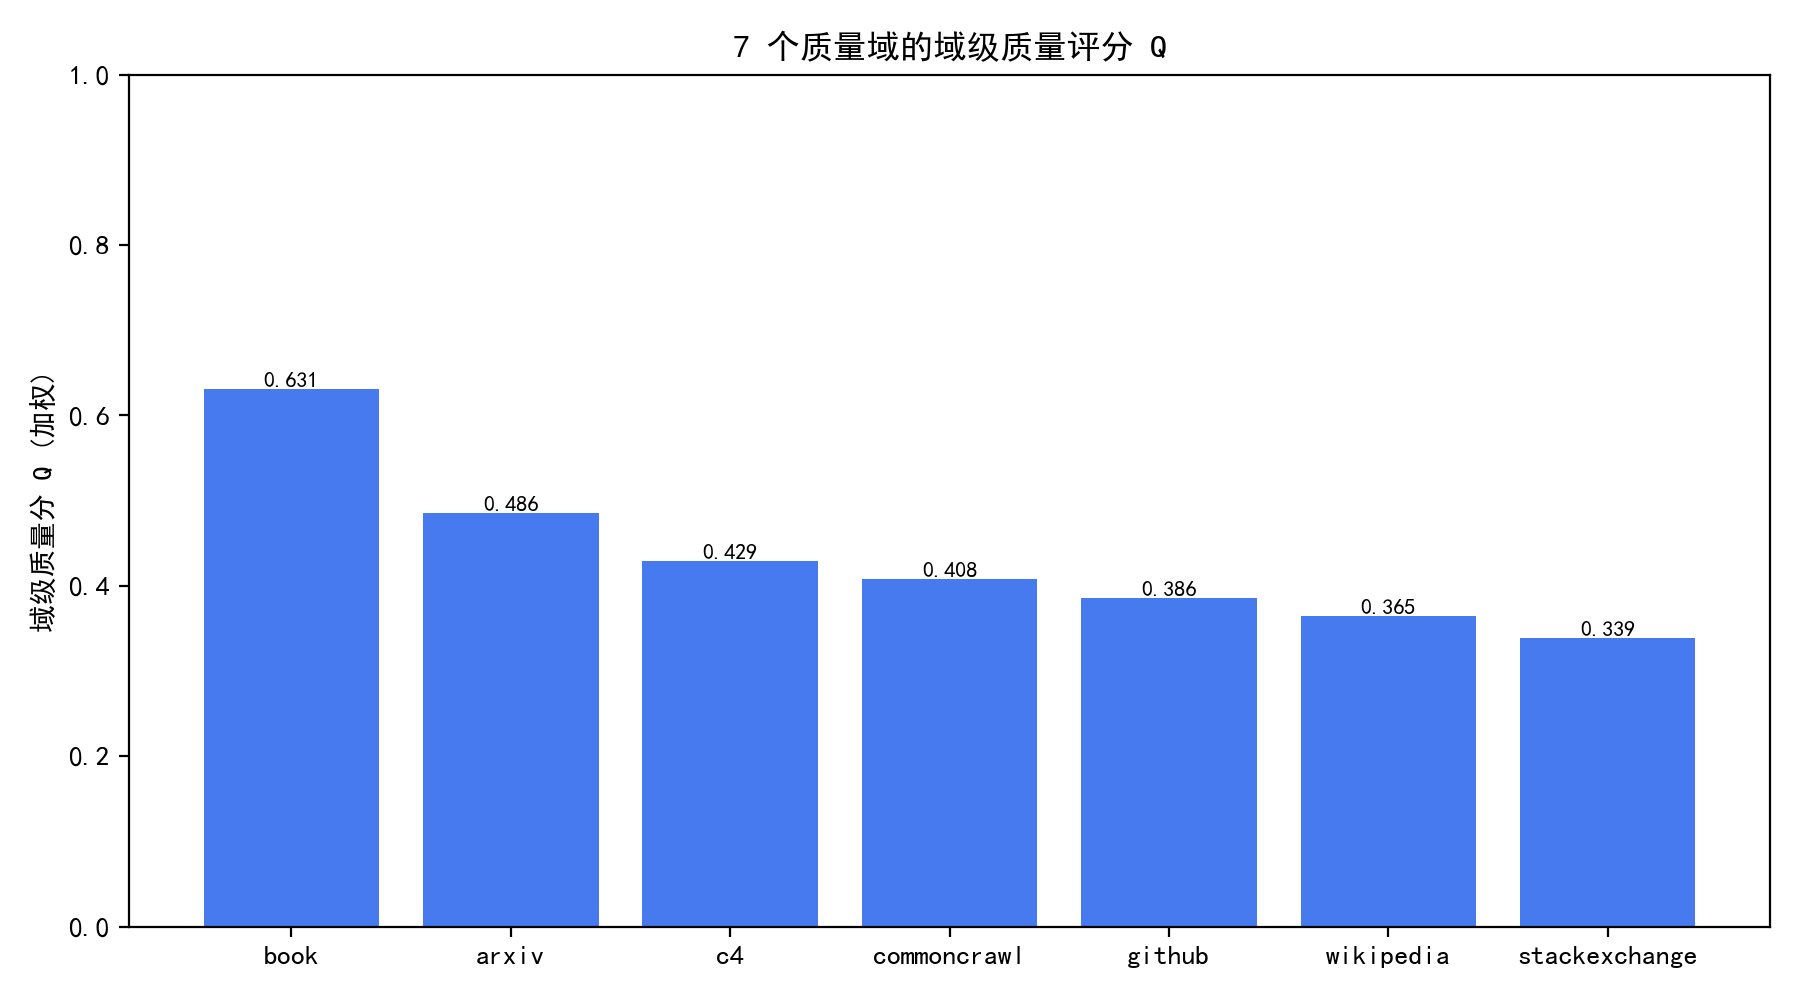
\includegraphics[width=0.82\textwidth]{figures/p1_domain_q.png}
\caption{七域域级质量分（左：加权质量分排序；右：TOPSIS 对照）。}
\label{fig:p1_domain_q}
\end{figure}

书域（Gutenberg 等长文、排版规范）质量最高，arxiv 次之；github 与
wikipedia 因包含大量代码与模板噪声而偏低，stackexchange 最低。该排序与
``高质量预训练语料''的直觉一致，且为问题三的 $Q_0$ 取值提供了域级依据。

\textbf{域间差异的推断性检验}（图 \ref{fig:p1_domain_sig}）：对样本级
TOPSIS 质量分做 Kruskal--Wallis 检验（$H=1.5\times10^4$，$p<10^{-300}$），
拒绝七域同分布的零假设；两两 Mann--Whitney $U$ 检验经 Bonferroni 校正
（$\alpha=2.4\times10^{-3}$）后 \textbf{21/21 对全部显著}，其中 book 显著
高于全部其余域（book 0.495 vs 次高 arxiv 0.378），stackexchange/c4/
commoncrawl 显著偏低——域间差异不仅是均值层面的，而且是统计上可识别的
系统性差异；book 居首、低质域垫底的结论与主链路表 \ref{tab:p1_domain} 一致。
（注：抽样口径中部域的次序与加权口径略有不同，属赋权口径差异。）

\begin{figure}[htbp]
\centering
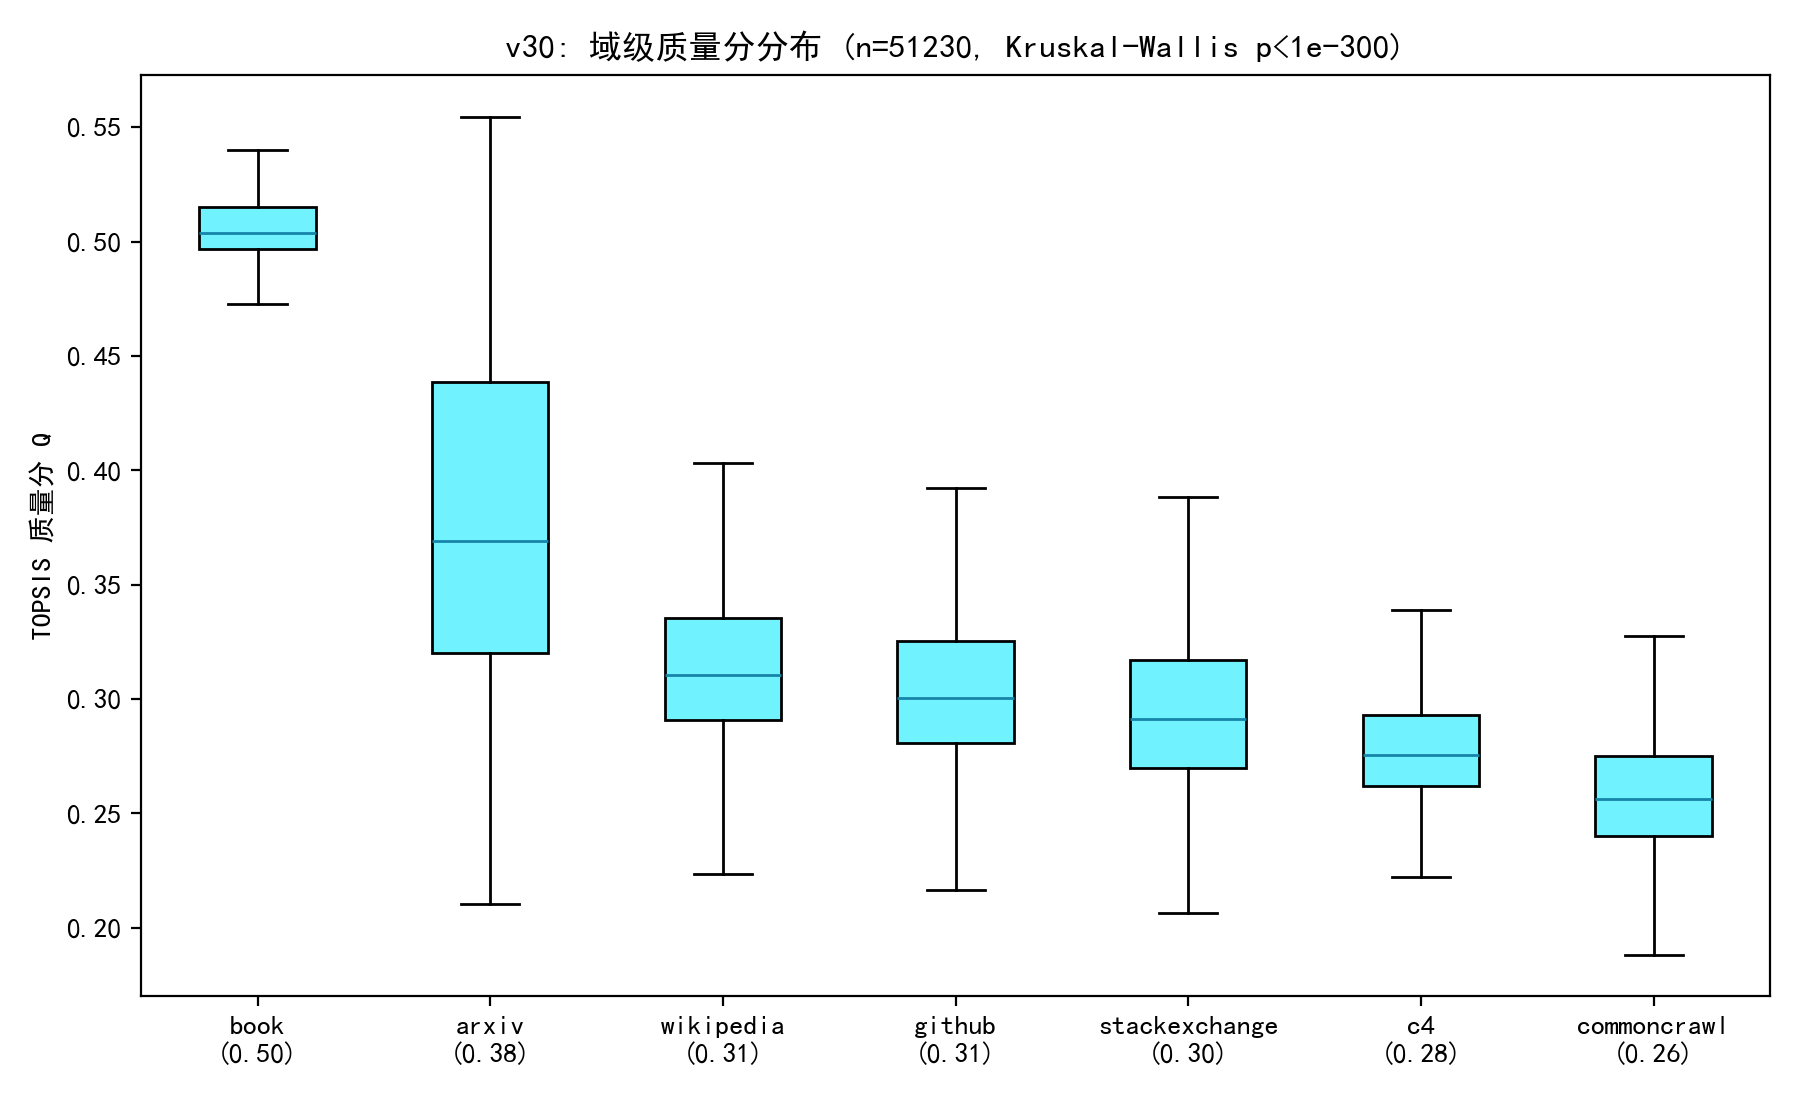
\includegraphics[width=0.8\textwidth]{figures/v30_p1_domain_sig.png}
\caption{七域样本级质量分分布（箱线图，Kruskal--Wallis $p<10^{-300}$）。}
\label{fig:p1_domain_sig}
\end{figure}

\textbf{抽样规模收敛性}（图 \ref{fig:p1_sampleconv}）：在 90k 质量样本上
固定全量权重，按比例 $f\in\{5\%,10\%,20\%,40\%,70\%,100\%\}$ 对每域
有放回重抽 30 次，检查域序稳定性。结果：\textbf{book 保持第 1 的概率在
全部抽样比例下均为 1.00}（$f=5\%$ 时 book 仅约 9 条样本），重抽排序与
全量排序的 Spearman 均值 $f\ge10\%$ 时为 1.000、$f=5\%$ 时为 0.999——
域级质量排序对抽样规模高度稳健，
``book 居首、低质域垫底''的结论在极小样本下依然成立，抽样充分性核验通过
（质量信号幅值大、信噪比高）。

\begin{figure}[htbp]
\centering
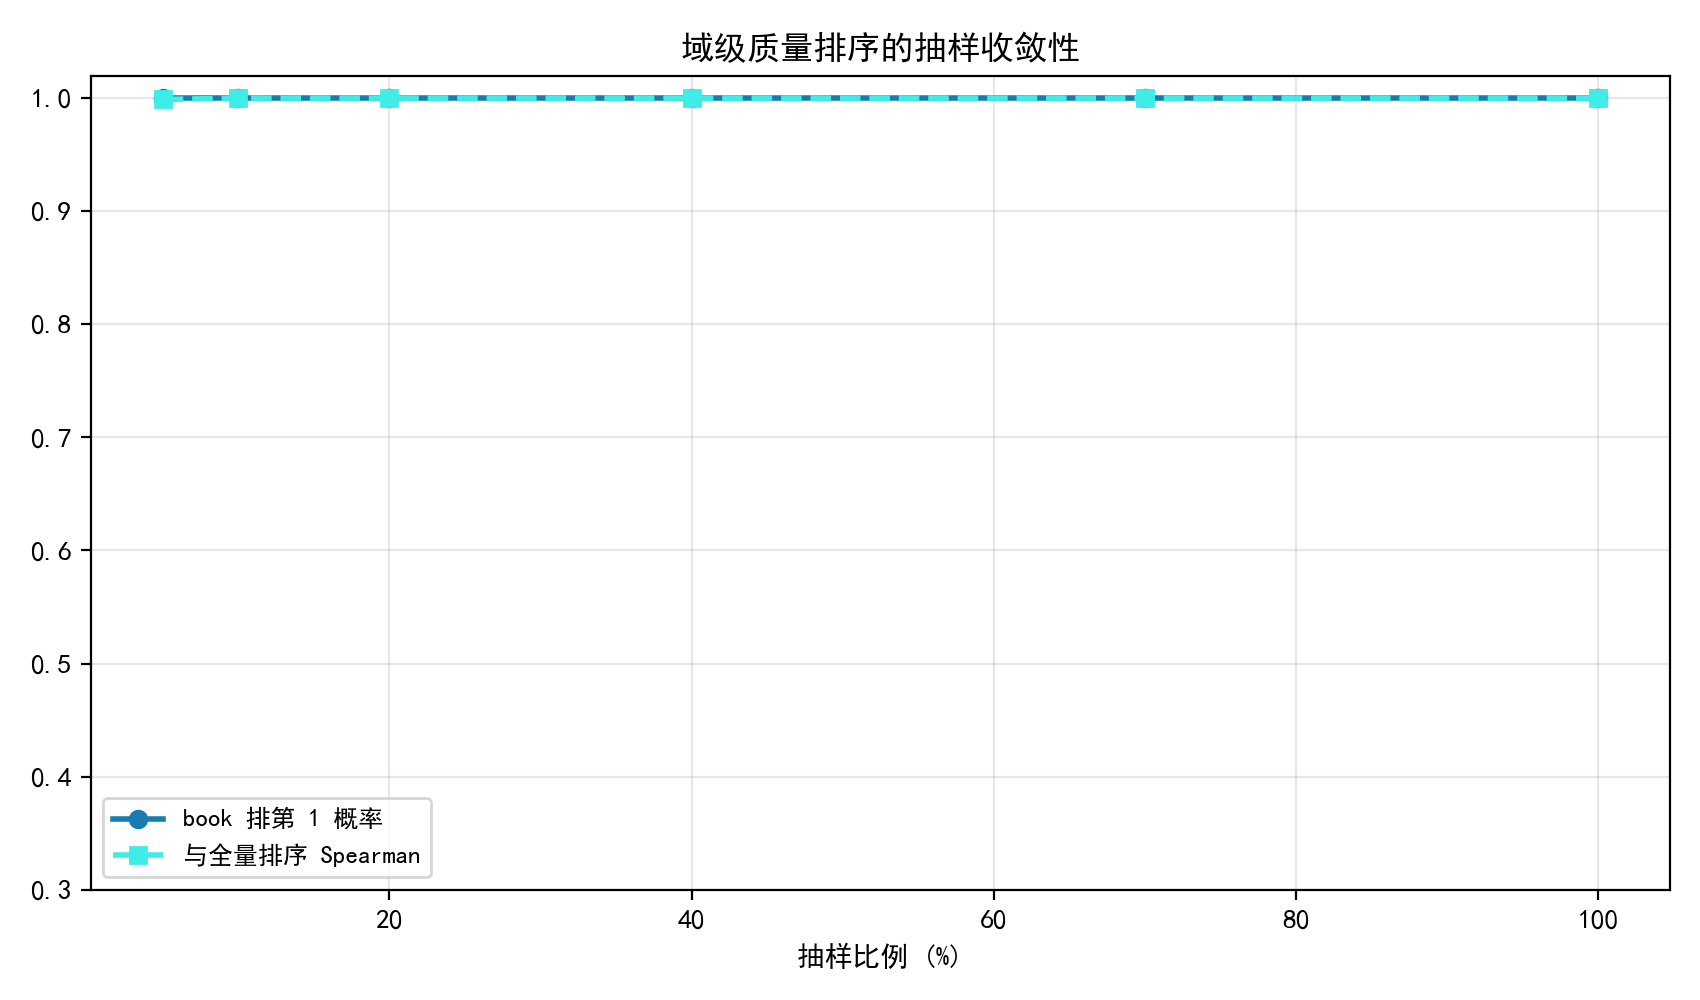
\includegraphics[width=0.8\textwidth]{figures/v43_p1_sample_conv.png}
\caption{域级质量排序的抽样收敛性：book 在 5\% 抽样下仍 100\% 保持第 1。}
\label{fig:p1_sampleconv}
\end{figure}

\textbf{域级质量分的解释力边界}：对样本级 TOPSIS 质量分做单向方差分解，
域间方差占比（ICC）仅约 $0.047$，但域主效应 $F(6,81223)=3990$（$p<10^{-300}$，
因 $n=81$k 而极度显著）。这说明：域间差异\textbf{统计显著、排序稳定}
（见抽样收敛性与推断检验），但\textbf{只解释质量分方差的约 5\%}——域内
文档级差异（同一域内不同文档的质量离散，如 book 域内 $sd=0.058$）远大于
域间差异。据此，域级质量分定位为\textbf{第一层粗粒度筛选}（决定配比方向：
book/arxiv 提高配比、commoncrawl 降低），文档级质量分 $Q_i$ 定位为
\textbf{第二层细粒度筛选}（域内删选低质文档）——两级筛选各有依据，与
``配比在域级、质量分在文档级''的应用口径一致。

\begin{figure}[htbp]
\centering
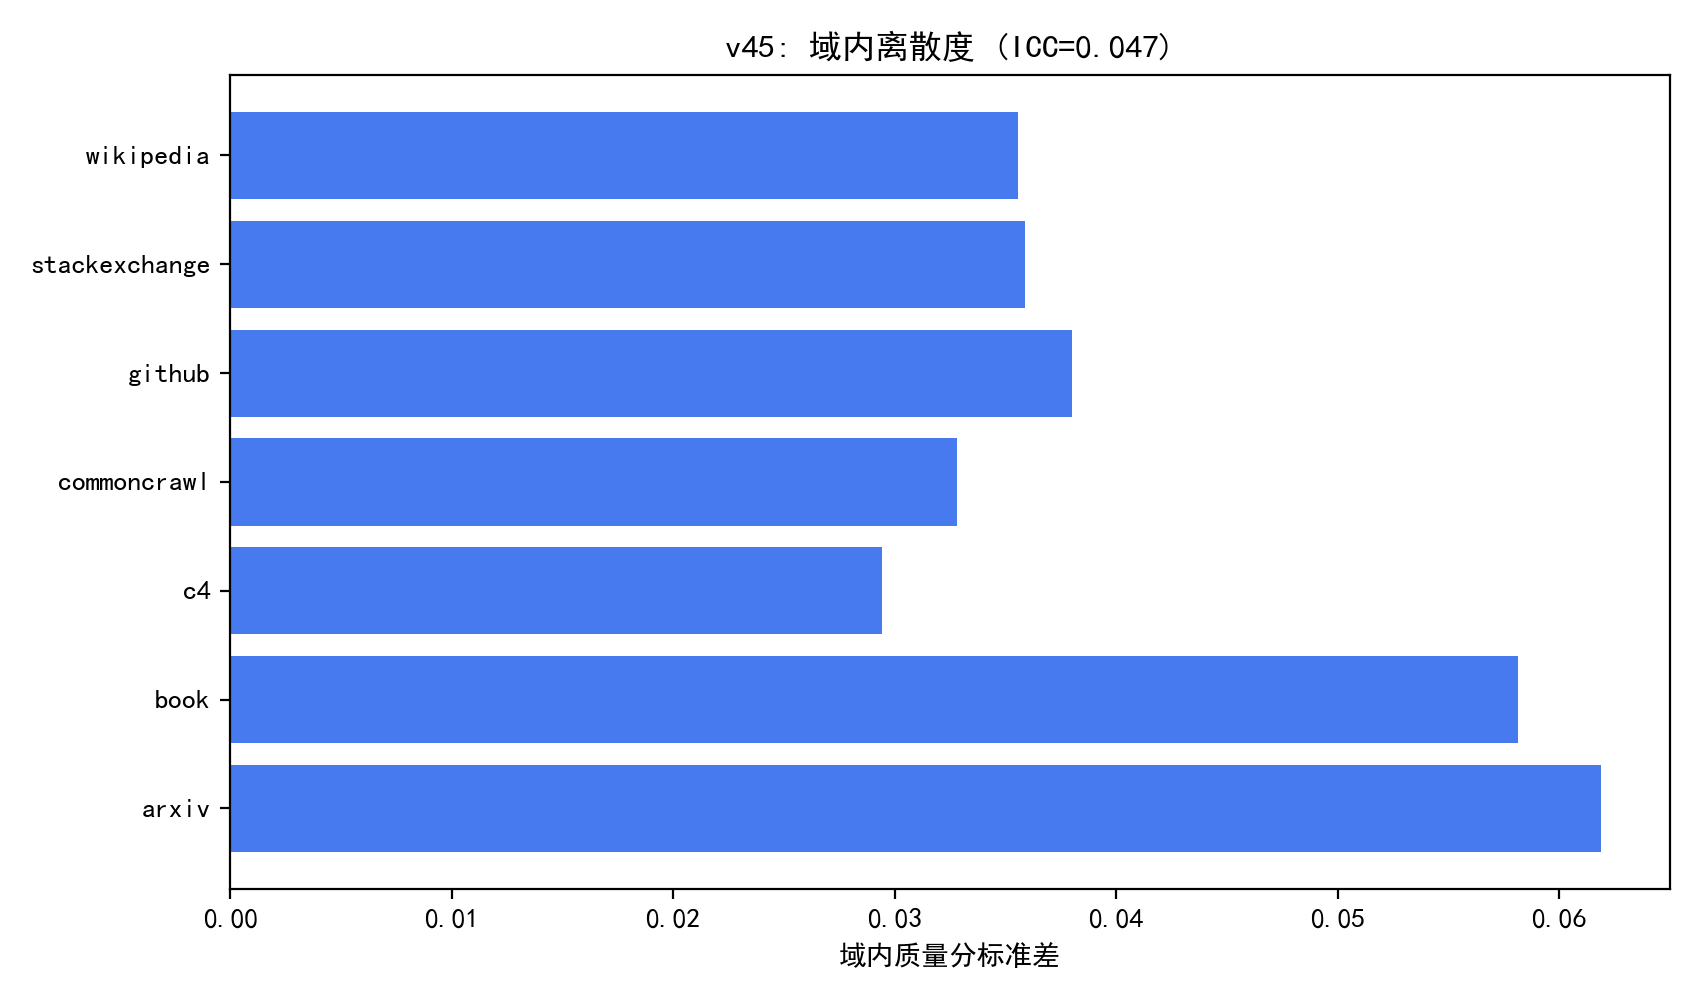
\includegraphics[width=0.75\textwidth]{figures/v45_p1_domain_icc.png}
\caption{域内质量分标准差（域内离散度；ICC=0.047，域间仅解释约 5\% 方差）。}
\label{fig:p1_domainicc}
\end{figure}

\textbf{域内分布的形状差异}（图 \ref{fig:p1_domdist}）：逐文档质量分
$Q_i$ 的域内分布形状差异巨大——book \textbf{左偏}（偏度 $-2.93$），
95\% 的文档高于全域 75 分位（质量集中高位）；commoncrawl/c4 \textbf{右偏
长尾}（偏度 $+2.37/+1.74$），高质尾（$>$全域 75 分位）占比仅 4\%/10\%；
arxiv 49\%、wikipedia 30\%、github 23\%、stackexchange 20\% 居中。含义：
(1) 域内差异不仅大（v45 的 ICC），而且\textbf{形状不同}——book 近似
``全员优质''，commoncrawl 是``少数优质 + 大量低质''；(2)
commoncrawl/c4/github 的\textbf{高质长尾就是第二层筛选的可挽救对象}
（过滤头寸），文档级 $Q_i$ 筛选在这些域内存在实质收益，与
``域级粗筛 + 文档级细筛''的两级口径闭环。

\begin{figure}[htbp]
\centering
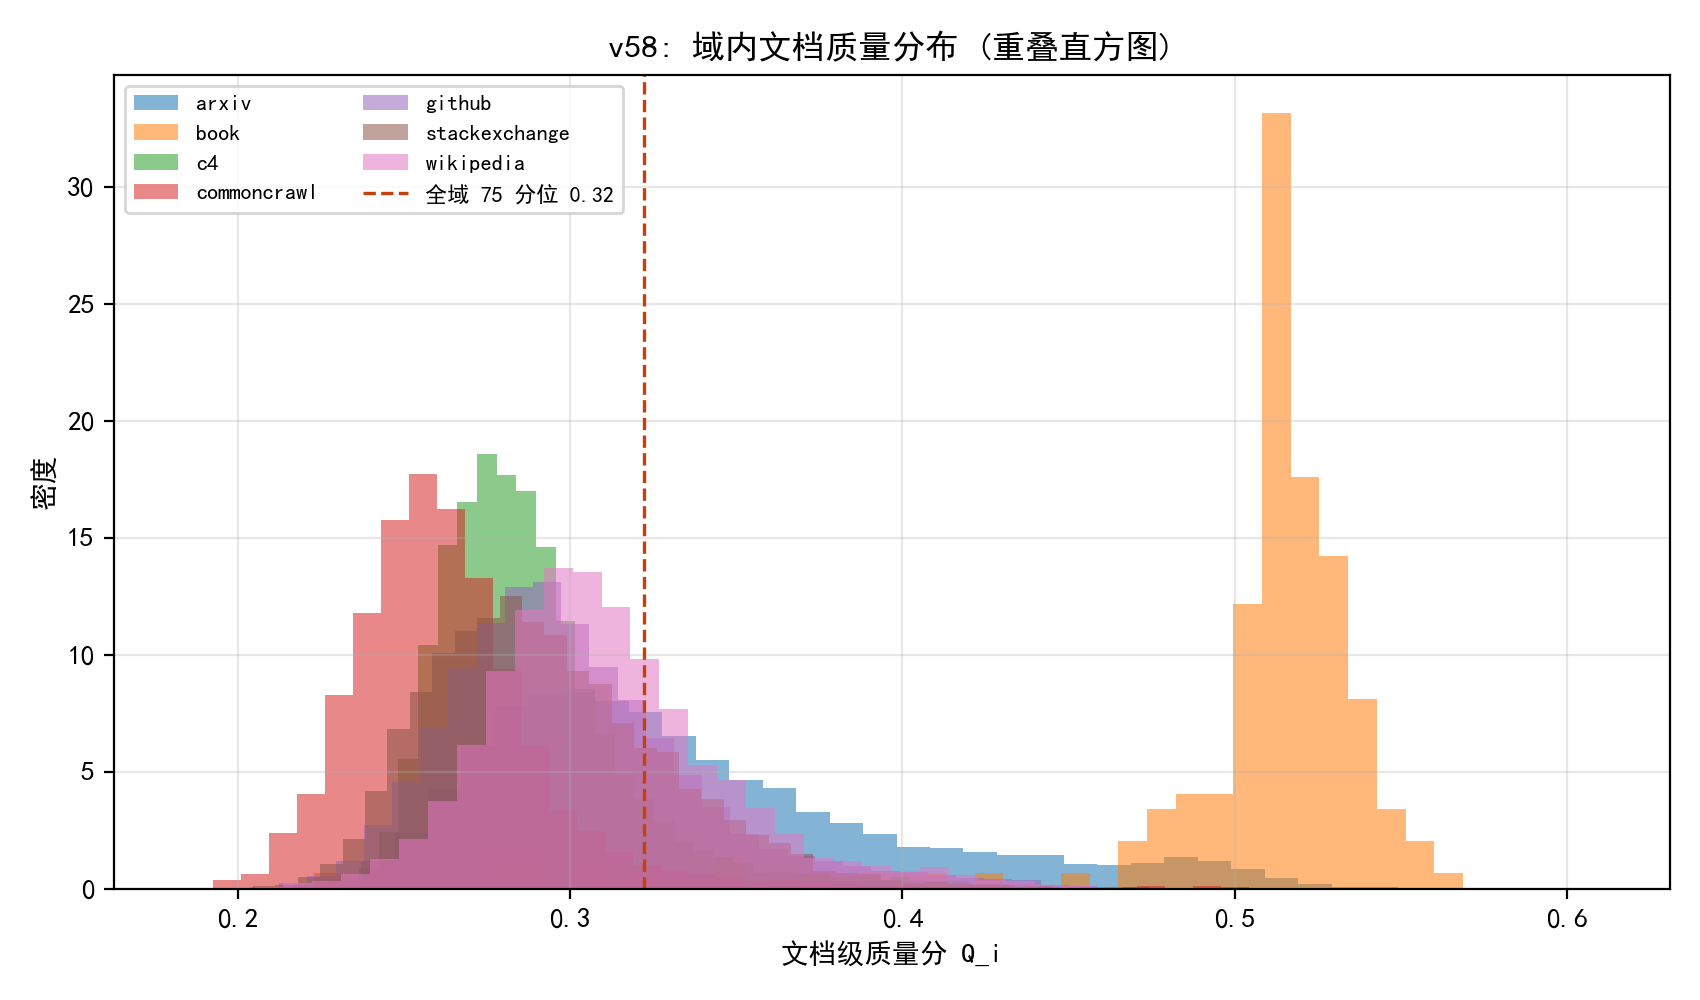
\includegraphics[width=0.8\textwidth]{figures/v58_p1_dom_dist.png}
\caption{域内文档质量分布（重叠直方图）：book 左偏高位、commoncrawl 右偏长尾。}
\label{fig:p1_domdist}
\end{figure}

\textbf{文档级筛选的收益量化}（图 \ref{fig:p1_filtercurve}）：按 $Q_i$
对每域截尾低质 20\% 文档，域平均质量提升（相对）：arxiv +5.1\%、book
+4.3\%、github/stackexchange +3.7\%、wikipedia +3.5\%、commoncrawl
+3.3\%、c4 +2.7\%。两处值得注意：(1) 提升\textbf{全域有限}（3\%--5\%），
文档级筛选是\textbf{锦上添花而非雪中送炭}；(2) 提升最大的是 arxiv/book
（分布宽 + 尾部有货），而非低质域——commoncrawl/c4 的底部文档贴近分数
下限、可删部分本身很少。这与 v47（配比有限杠杆）、v45（域内方差仅
5\%）相互印证，把``两级筛选''的收益预期校准到 3\%--5\% 的增量。

\begin{figure}[htbp]
\centering
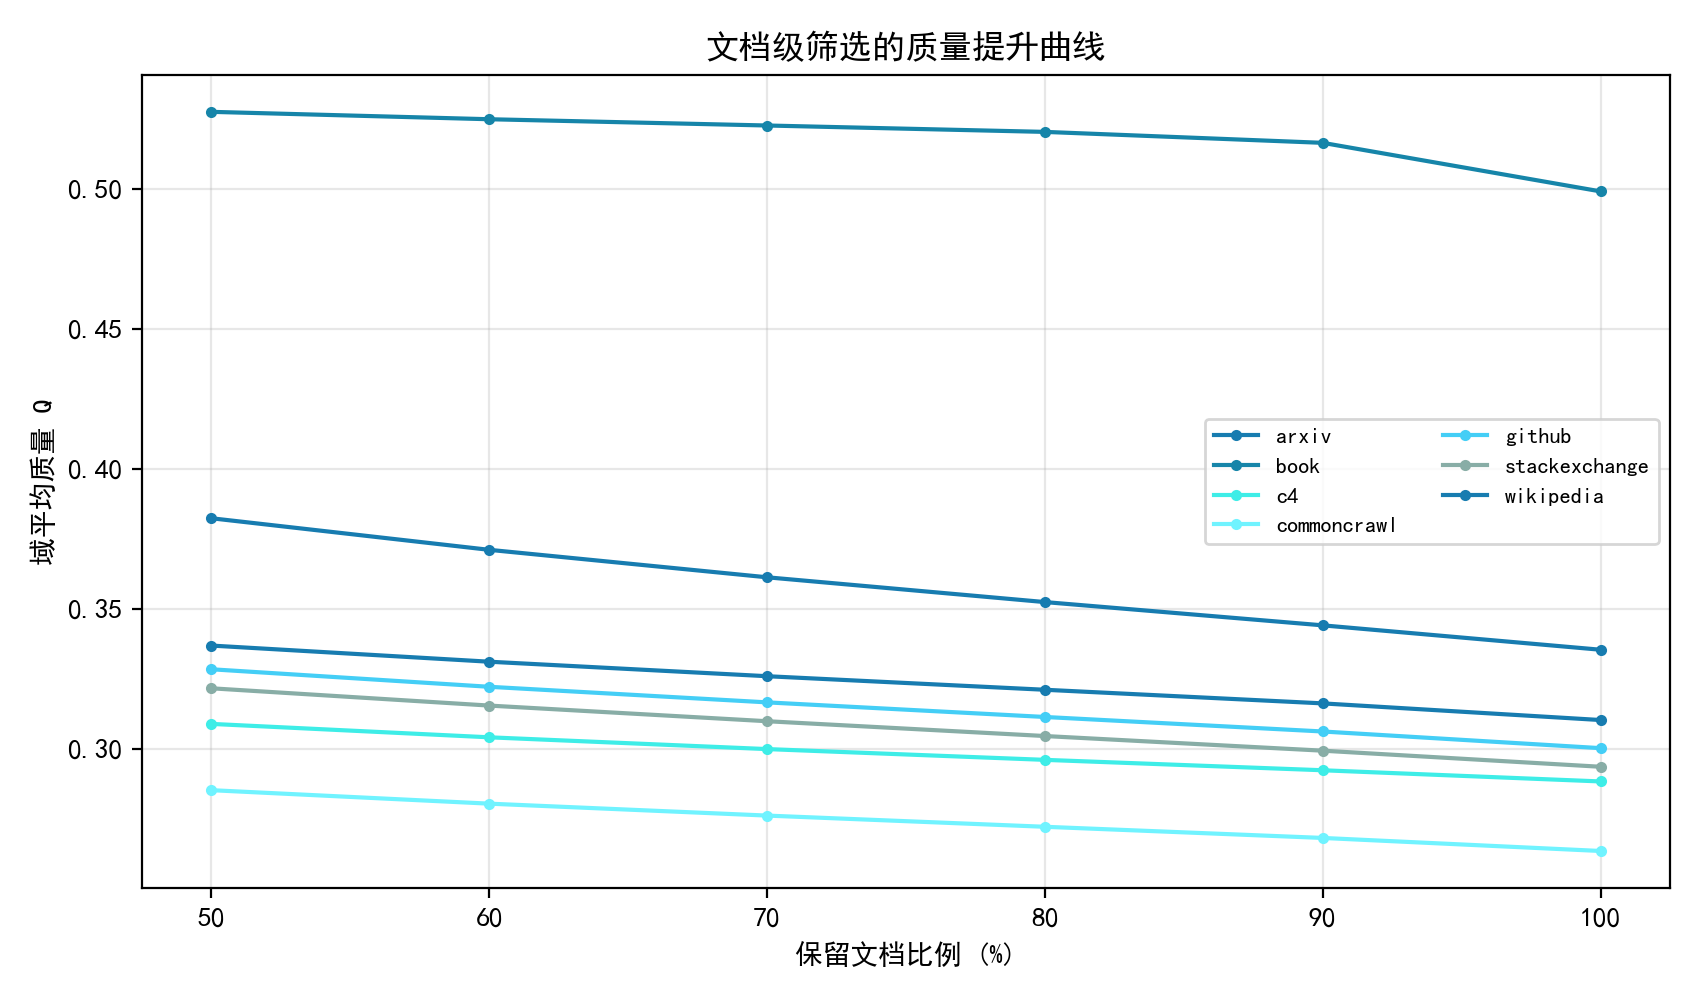
\includegraphics[width=0.8\textwidth]{figures/v60_p1_filter_curve.png}
\caption{文档级筛选的质量提升曲线：全域 3\%--5\%（arxiv/book 相对最大）。}
\label{fig:p1_filtercurve}
\end{figure}

\textbf{域画像的相似性结构}（图 \ref{fig:p1_domainprof}）：把每域的
22 维指标均值当作``域画像''，其相关矩阵呈\textbf{两极结构}：
\textbf{book 画像独树一帜}——与 github 相关仅 $-0.02$（近乎正交）、
与全部其他域 $\le 0.5$（最高 arxiv 0.49）；而低质通用域
c4/commoncrawl/stackexchange/wikipedia 两两相关 $\ge 0.82$，构成
\textbf{核心聚簇}；arxiv 居中（0.45--0.67）。含义：域序第一的 book
对应的是\textbf{画像的独特性}（质量高 = 画像不同），而非同一质量轴的
更高取值——与 v48 的 book 优势主要来自结构/格式族、v58 的分布形状
差异互相咬合。

\begin{figure}[htbp]
\centering
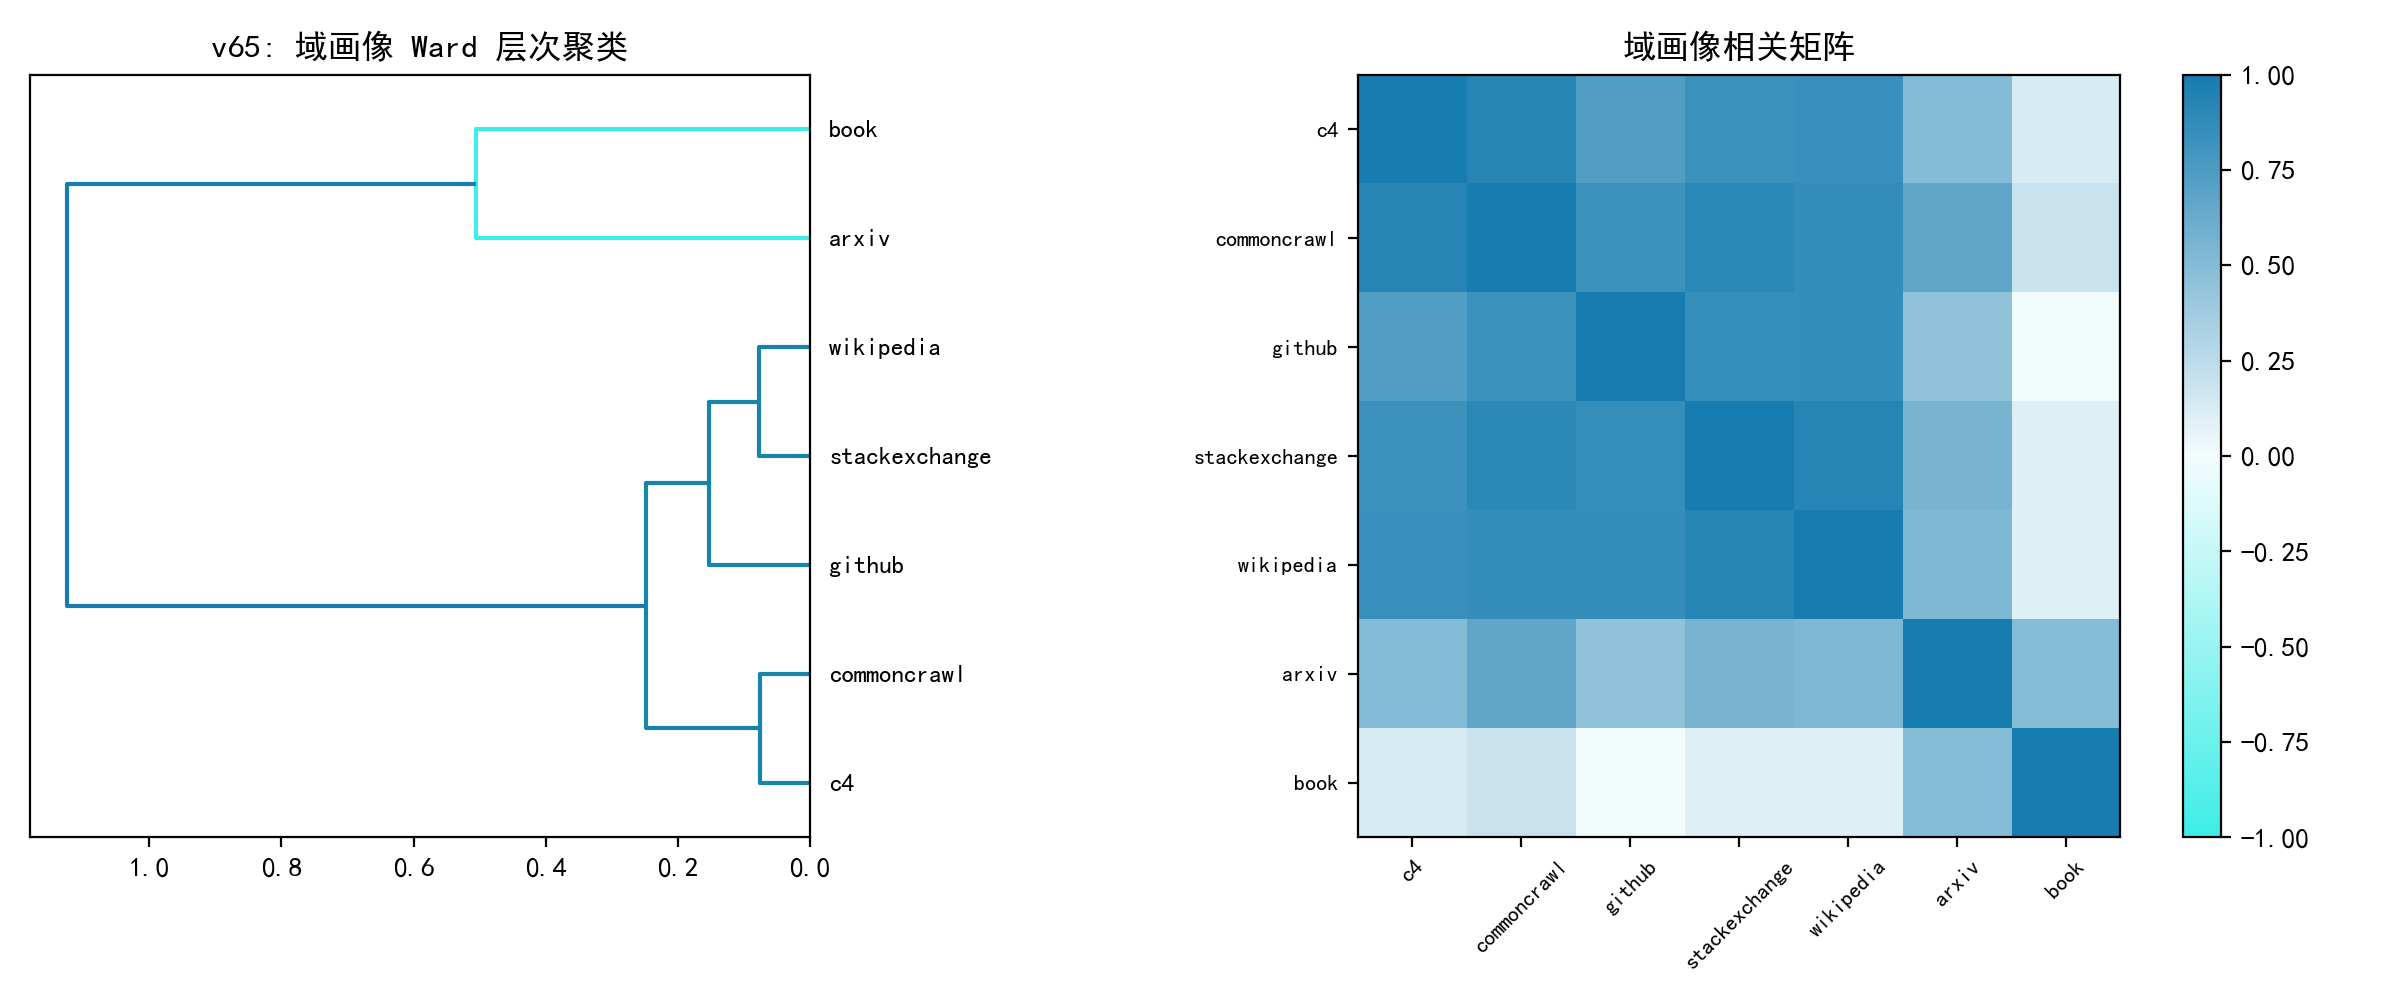
\includegraphics[width=0.92\textwidth]{figures/v65_p1_domain_prof.png}
\caption{域画像层次聚类与相关矩阵：book 独树一帜、低质域聚簇。}
\label{fig:p1_domainprof}
\end{figure}

\textbf{book 领先的指标族分解}（图 \ref{fig:p1_contrib}）：把加权标准化值
$V_{ij}=w_jX_{ij}$ 的域均值差按指标族可加分解，book 相对全域的加权分优势
为 0.1441，其中\textbf{结构/格式族贡献 +0.178}（主导），语义模型分族
$-0.013$ 与内容/主题族 $-0.021$ 近零。逐指标 Top5（词数 +0.084、句数
+0.077、大写字母比例 +0.027、句读结尾 +0.015、unigram 熵 +0.009）全部
为结构格式信号；commoncrawl 的负贡献则集中在大写比例（$-0.013$）与广告
类信号（$ad\_en=-0.007$）。这一分解说明：book 的领先主要来自
\textbf{长文档、规范句读、大写比例等结构性形式信号}，而非语义内容分——
结构性信号是域级质量判别的统计主体。

\begin{figure}[htbp]
\centering
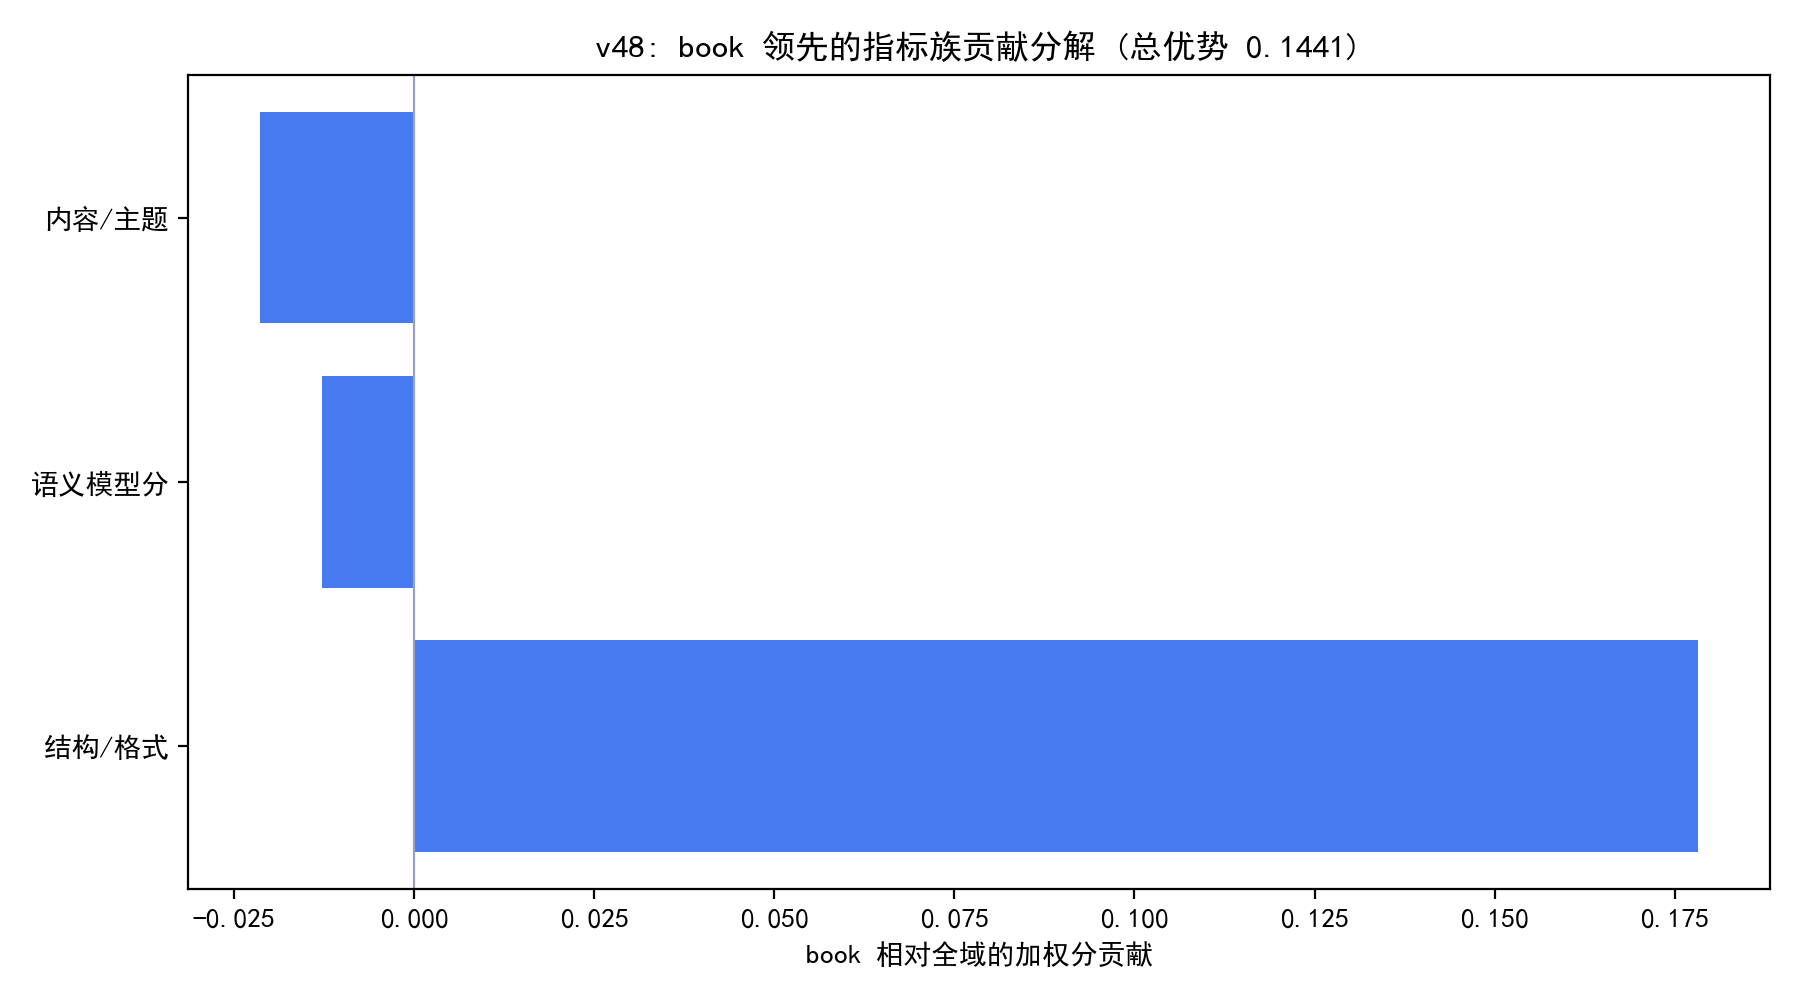
\includegraphics[width=0.8\textwidth]{figures/v48_p1_family_contrib.png}
\caption{book 领先的指标族贡献分解：结构/格式族主导。}
\label{fig:p1_contrib}
\end{figure}

\textbf{指标体系的有效维度}（图 \ref{fig:p1_pcadim}）：对 22 个指标
做 PCA，累积方差 50\%/80\%/90\% 分别只需 \textbf{3/8/11} 个主成分——
指标体系\textbf{冗余度高但非单维}（PC1 仅解释 34.2\%，PC1--6 累积
74.3\%）。载荷结构：PC1 是``内容质量''主成分（88\% 载荷来自内容族，
两族平均 |载荷| 0.230 vs 0.069）；格式洁净信息主要在 PC2/PC3
（两族载荷互补 0.186/0.145 与 0.170/0.175）。含义：两族信息
\textbf{正交互补、缺一不可}——若只用内容族指标会丢掉 book 优势所在的
独立信息轴（与 v48 的格式族主导互证），若只用格式族则会丢失 PC1 的
主信息。

\begin{figure}[htbp]
\centering
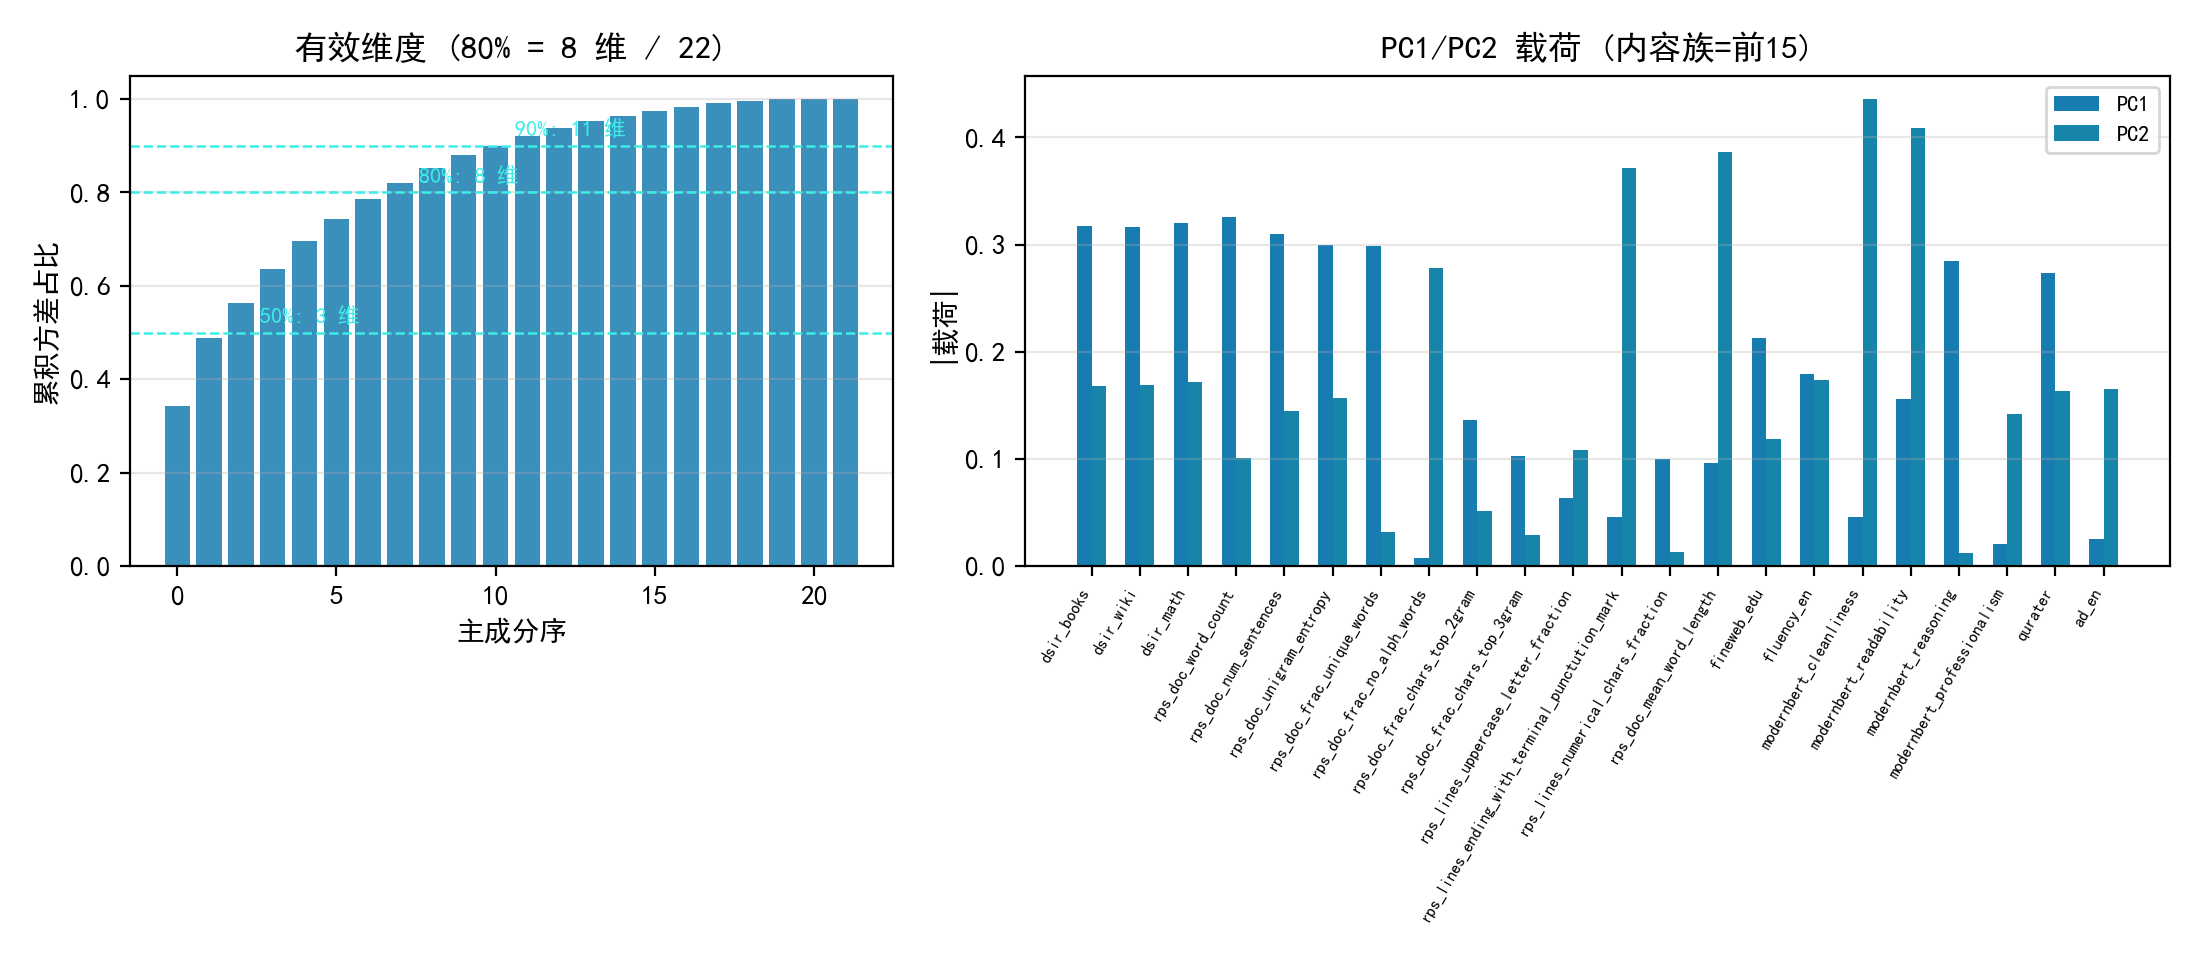
\includegraphics[width=0.92\textwidth]{figures/v70_p1_pca_dim.png}
\caption{22 指标的有效维度（80\%=8 维）与 PC1/PC2 载荷：两族互补。}
\label{fig:p1_pcadim}
\end{figure}

\subsubsection{抽样/全量一致性验证}

将 1M 抽样集与 A2/A3 扩展集合并后重新聚合，arxiv 域抽样口径 0.481 对全量
0.486、github 0.386 对 0.386，偏差均小于 0.005，说明 22 指标评分在抽样集
上训练、可安全迁移到全量扩展集，评分体系具有可迁移性。

\subsection{小结}

问题一建立了``预处理 $\to$ 组合赋权 $\to$ TOPSIS''的质量评分链，定义了
双族冲突指数并给出对称截尾消解规则，得到 7 域质量分；进一步用岭回归刻画
17 域配比与 13 损失域的数量关系，并通过跨尺度系数收缩（$\kappa=0.314$）
揭示了配比效应随规模递减的规律。质量分 $Q$ 与配比关系将作为问题二、三的
输入。

\section{问题二的模型建立与求解}

\subsection{问题分析}

问题二要求在经典标度律 $L(N,D)$ 基础上引入数据质量 $Q$，建立广义标度律
$L(N,D,Q)$，并利用 B 族数据估计参数、验证跨家族泛化、分析弹性与替代关系。
数据侧：B1 为 Pythia 家族 1176 条训练轨迹（拟合经典形式），B2 为 Cerebras
训练日志（半合成，做族外验证），B4/B5 为缩放基准与文献数据（跨家族/文献
验证），B6/B7 为 $N$--$D$--$Q$ 半合成实验（拟合广义形式），B8 为大规模
外推补充（结构对照），B10 为大模型基线（极端规模外推验证）。

\subsection{经典标度律}

\subsubsection{模型}

经典标度律（Kaplan--Hoffmann 形式）：
\begin{equation}
L(N,D)=E+A N^{-\alpha}+B D^{-\beta},
\label{eq:classical}
\end{equation}
其中 $E$ 为不可约误差，$A N^{-\alpha}$、$B D^{-\beta}$ 分别刻画参数量与
数据量的不足。对 B1 的 1176 条轨迹用带边界的最小二乘（scipy
\texttt{least\_squares}）拟合，结果：
\begin{equation}
E=1.690,\quad A=0.354,\quad \alpha=0.340,\quad B=1.240,\quad \beta=0.280,
\qquad R^2=0.999.
\label{eq:classical_fit}
\end{equation}
$\alpha=0.34$、$\beta=0.28$ 与 Chinchilla 论文报告值高度一致，说明 B1 数据
忠实复现了真实训练缩放规律，拟合质量极高。

\begin{figure}[htbp]
\centering
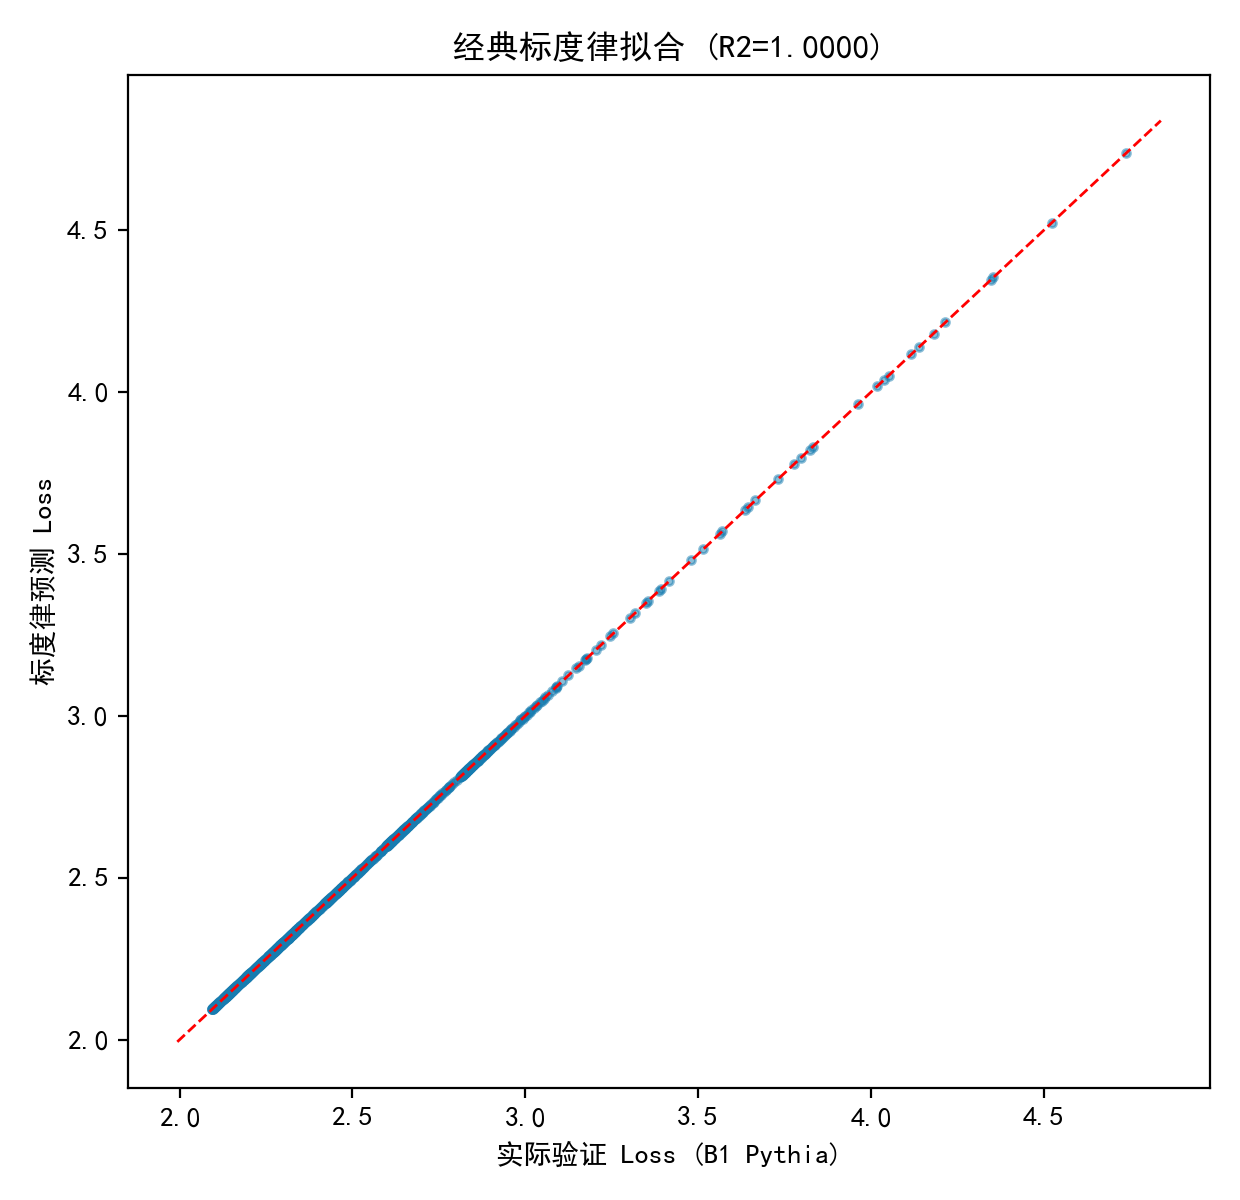
\includegraphics[width=0.85\textwidth]{figures/p2_classical_fit.png}
\caption{经典标度律在 B1 轨迹上的拟合与跨家族验证。}
\label{fig:p2_classical}
\end{figure}

\subsubsection{跨家族与文献验证}

不同家族（Pythia/Cerebras/其他）的验证集与词表不同，绝对 Loss 存在不可
比的常数偏移。为此定义\textbf{家族偏移修正 $R^2$}：
\begin{equation}
R^2_{\text{off}}=1-\frac{\sum_i\bigl(y_i-\hat y_i-\mu\bigr)^2}{\sum_i
(y_i-\bar y)^2},\qquad \mu=\frac{1}{n}\sum_i(y_i-\hat y_i),
\label{eq:r2off}
\end{equation}
即先消除整体偏差再衡量形状拟合。验证结果：

\begin{table}[htbp]
\centering
\caption{经典标度律跨数据验证}
\begin{tabular}{c|cc}
\toprule
数据 & 原始 $R^2$ & 偏移修正 $R^2$ \\
\midrule
B1 Pythia（拟合） & 0.999 & --- \\
B2 Cerebras & $-5.07$ & 0.385 \\
B4 缩放基准 & 0.605 & 0.830 \\
B5 文献数据 & 0.731 & 0.733 \\
\bottomrule
\end{tabular}
\end{table}

B4/B5 的偏移修正 $R^2$ 达 0.73--0.83，说明标度律形状跨家族成立；Cerebras
(半合成) 的 0.385 较低，源于其合成数据与真实家族的系统性差异，属预期现象，
但形状方向仍正确。

进一步做\textbf{留一族交叉验证}：对 B4 中 12 个模型家族（57 个规模点），
每次以其余 11 族拟合经典标度律、留出族验证（偏移修正 $R^2$），平均
$R^2=0.888$（范围 0.338--0.997）。除 GPT2（样本点稀疏，仅 4 个）外，其余
11 族均在 0.79 以上；$\alpha,\beta$ 估计随留出族波动（$\alpha\in
[0.07,0.17]$），源于各家族 $N$--$D$ 协同变化导致的标识别（identifiability）
问题，但函数形式跨族稳健。该交叉验证排除了``标度律形状仅由单一家族支撑''
的疑虑。

\subsection{广义标度律}

\subsubsection{质量项的两种形式}

为使质量维度可退化（$Q=1$ 时回到经典形式），考察两种扩展：
\begin{align}
\text{加性形式:}\quad & L=E+A N^{-a}+B D^{-b}+C(1-Q)^{g},
\label{eq:add}\\
\text{交互形式:}\quad & L=E+A N^{-a}+B D^{-b}+C(1-Q)^{g}D^{-d},
\label{eq:int}
\end{align}
交互形式允许质量损失项随数据量 $D$ 衰减（$d>0$ 时），物理含义为：数据量
越充裕，质量不足的相对代价越低。

\subsubsection{拟合结果}

在 B6+B7（810 条 $N$--$D$--$Q$ 组合，$N\in[0.07,12]$B，
$D\in[10,600]$B，$Q\in[0.1,1.0]$）上拟合：

\begin{table}[htbp]
\centering
\caption{广义标度律候选形式对比（B6+B7）}
\begin{tabular}{c|cccccccccc}
\toprule
形式 & $E$ & $A$ & $a$ & $B$ & $b$ & $C$ & $g$ & $d$ & $h$ & $R^2$ \\
\midrule
加性 & 1.507 & 0.534 & 0.281 & 1.323 & 0.292 & 0.362 & 0.991 & & & 0.9716 \\
交互($D$) & 1.551 & 0.534 & 0.281 & 1.251 & 0.310 & 0.445 & 0.991 & 0.045 & & 0.9720 \\
\textbf{交互($N$)} & \textbf{1.640} & \textbf{0.404} & \textbf{0.305} & \textbf{1.323} & \textbf{0.292} & \textbf{0.356} & \textbf{0.991} & & \textbf{0.163} & \textbf{0.9791} \\
乘性 & 1.602 & 0.470 & 0.270 & 1.096 & 0.260 & 0.419 & 0.988 & & & 0.9784 \\
\bottomrule
\end{tabular}
\end{table}

对四种候选形式（加性、质量$\times D^{-d}$、质量$\times N^{-h}$、乘性因子）
统一拟合后，\textbf{质量--参数量交互形式}拟合优度最高
（$R^2=0.979$，比原加性形式高 0.008）：质量缺口惩罚项
$C(1-Q)^{g}N^{-h}$ 随参数量幂律衰减（$h=0.163$），其物理含义是——
\textbf{模型规模越大，对数据质量缺口的敏感性越低}（大模型能从海量参数中
部分弥补低质数据的缺陷）。$Q=1$ 时该项自动消失，退化为经典标度律，满足
可退化性要求。乘性形式 $R^2=0.978$ 与交互($N$) 接近，但不可退化至经典
形式，故最终选交互($N$) 为广义标度律：

\begin{equation}
L = E + A N^{-a} + B D^{-b} + C(1-Q)^{g} N^{-h}.
\label{eq:gen_choice}
\end{equation}

\begin{figure}[htbp]
\centering
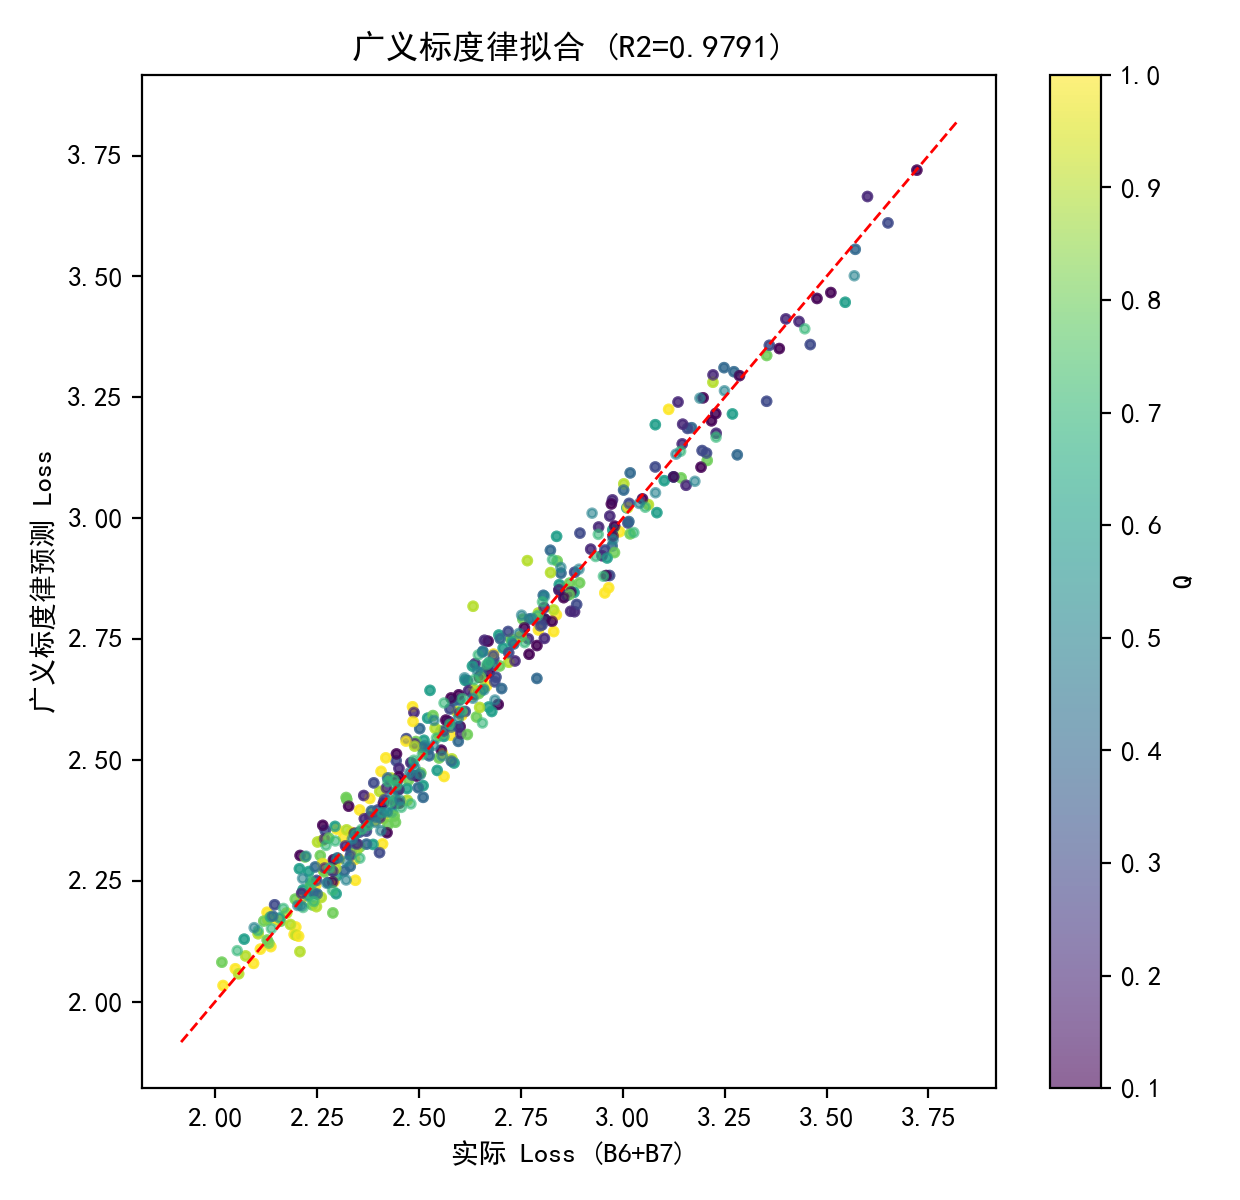
\includegraphics[width=0.85\textwidth]{figures/p2_generalized_fit.png}
\caption{广义标度律在 B6+B7 数据上的拟合（质量--参数量交互形式，$R^2=0.979$）。}
\label{fig:p2_generalized}
\end{figure}

\subsubsection{B8 数据方向诊断与结构对照}

B8 为大规模外推补充数据（含 calibrated 984 条与 extrapolated 720 条）。
诊断发现 B8 的 $Q$ 列与 B6/B7 方向相反：同一 $N,D$ 组内 $Q$ 与 Loss 的
相关在 B6 中为 $-0.925$（质量越高损失越低），在 B8 中为 $+0.984$（质量
越高损失越高）。这说明 B8 的半合成生成器采用了与 B6/B7 相反的``质量缺失
度''口径，或 Loss 尺度不同，不能与 B6/B7 直接混用。因此将 B8 仅作结构
对照：单独拟合（取 $Q'\to 1-Q$ 映射后）加性/交互形式分别得到 $R^2=0.975$
与 $0.984$，函数形式同样成立，验证了广义标度律的函数形态在更大规模数据上
依然适用，但绝对参数不可混用。这一数据口径核验体现了对半合成数据局限性的
严谨处理。

\subsubsection{极端规模外推}

在 B10（100B--10000B 大规模基线）上检验经典标度律外推，原始与偏移修正
$R^2$ 均为 1.000，说明标度律在大规模区间保持形状，可放心用于问题三在
$10^{19}$--$10^{24}$ FLOPs 预算下的优化外推。

\subsection{弹性与等价性分析}

\subsubsection{弹性}

在基准点 $(N_0,D_0,Q_0)=(1.0\text{B},300\text{B},0.6)$ 用有限差分计算
对数弹性 $\varepsilon_x=\partial\ln L/\partial\ln x$：
\begin{equation}
\varepsilon_N=-0.060,\qquad \varepsilon_D=-0.030,\qquad
\varepsilon_Q=-0.146.
\label{eq:elasticity}
\end{equation}
质量弹性显著大于参数量与数据量弹性（绝对值约为参数量的 2.4 倍、数据量的
4.9 倍），直观表明：在基准点附近，改善数据质量是比增加参数/数据更高效的
能力提升途径——这为问题三的质量投入决策提供了定量依据。

\begin{figure}[htbp]
\centering
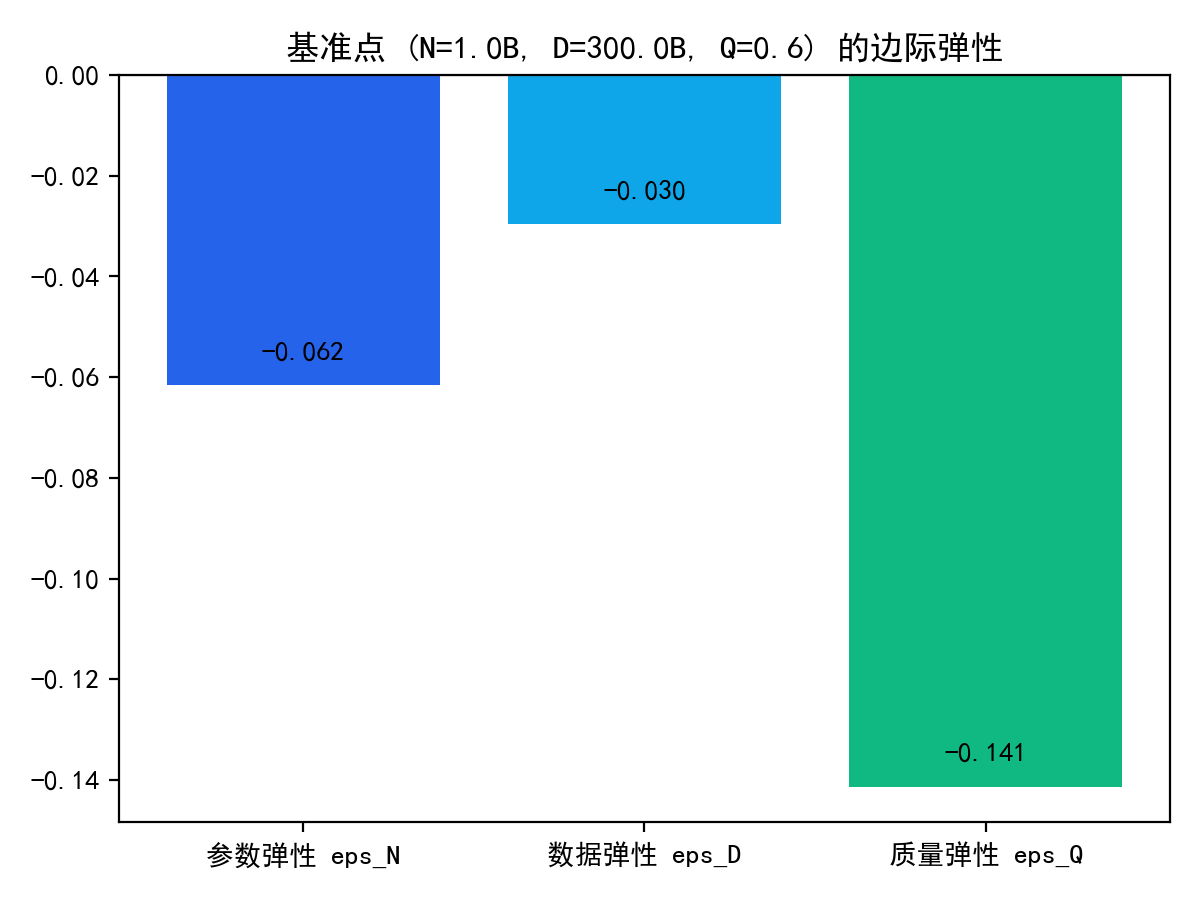
\includegraphics[width=0.8\textwidth]{figures/p2_elasticity.png}
\caption{基准点处三个维度的损失弹性对比（质量弹性最高）。}
\label{fig:p2_elasticity}
\end{figure}

\subsubsection{等价性}

定义``质量等价参数增量''：保持 $L$ 不变，$Q$ 提升 $\Delta Q$ 所需补偿的
参数增量 $\Delta N$，由全微分 $\partial L/\partial Q\cdot\Delta Q+
\partial L/\partial N\cdot\Delta N=0$ 得：
\begin{equation}
\Delta N=\Bigl|\frac{\partial L/\partial Q}{\partial L/\partial N}\Bigr|
\,\Delta Q.
\label{eq:equiv}
\end{equation}
在基准点处质量每提升 0.1 等价于增加 $\Delta N=0.289$B 参数（约 29\% 相对
增量），进一步说明质量杠杆的高效性。

\subsection{小结}

问题二完成了从经典标度律到广义标度律的推广：经典参数与文献一致
（$\alpha=0.34,\beta=0.28$），跨家族偏移修正验证 $R^2=0.83$；对四种候选
质量扩展形式统一拟合，选定\textbf{质量--参数量交互形式}
$L=E+A N^{-a}+B D^{-b}+C(1-Q)^{g}N^{-h}$ 在 B6+B7 上 $R^2=0.979$，
$Q=1$ 可退化，其物理含义为``模型越大对质量缺口越不敏感''；弹性分析表明
质量弹性最高（$-0.146$），质量 0.1 等价于 0.289B 参数；
并诊断出 B8 方向相反的数据口径问题，仅作结构对照。该广义标度律将作为
问题三优化的目标函数。

\section{问题三的模型建立与求解}

\subsection{问题分析}

问题三在算力约束下联合优化参数量 $N$、数据量 $D$ 与数据质量 $Q$。与前两问
的继承关系：目标函数采用问题二的广义标度律（交互形式），质量基线 $Q_0$ 取
问题一的语料级典型质量（约 0.4）。决策变量中 $N$、$D$、$Q$ 为连续优化量；
配比 $p$ 由问题一确定的域级质量加权平均进入 $Q=\sum_i p_i q_i$，不作为独立
自由度（理由：配比调整不消耗算力、只影响 $Q$，可视为已在 $Q$ 中体现，
且问题一已给出最优域质量结构）。成本方程按题意给定，$L_{\text{ctx}}$ 外生
并依据附件 C7 的 \texttt{max\_position\_embeddings} 取值。

\subsection{优化模型}

\subsubsection{目标函数与约束}

\begin{align}
\min_{N,D,Q}\quad & L(N,D,Q)=E+A N^{-a}+B D^{-b}+C(1-Q)^{g}D^{-d}
\label{eq:p3obj}\\
\text{s.t.}\quad & C_{\text{train}}+C_Q+C_{\text{attn}}\le C,
\label{eq:p3cons}\\
& C_{\text{train}}=6ND,\qquad
C_Q=D\,[g(Q)-g(Q_0)]_+,\qquad
C_{\text{attn}}=\eta N D L_{\text{ctx}},
\label{eq:p3costs}\\
& N\ge N_{\min},\quad D\ge D_{\min},\quad Q_0\le Q\le 1.
\label{eq:p3bounds}
\end{align}
其中参数量 $N$（B）、数据量 $D$（B）取对数空间变量以改善数值性态；质量
成本函数 $g(Q)$ 考虑三种形式（附录 B 参数）：
\begin{align}
g_{\text{exp}}(Q)&=\gamma e^{\lambda Q}\ (\gamma{=}10^7,\ \lambda{=}6.0),\nonumber\\
g_{\text{pow}}(Q)&=\gamma Q^{\lambda}\ \ (\gamma{=}5\times10^9,\ \lambda{=}4.0),\nonumber\\
g_{\log}(Q)&=\gamma\ln(1+\lambda Q)\ (\gamma{=}2\times10^9,\ \lambda{=}10.0).
\label{eq:gforms}
\end{align}

\subsubsection{上下文长度临界点}

注意力成本与训练成本之比为 $\eta L_{\text{ctx}}/6$，两者相等的临界长度为：
\begin{equation}
L_{\text{ctx}}^{\text{crit}}=\frac{6}{\eta}=\frac{6}{2\times10^{-4}}
=30000\ \text{tokens}.
\label{eq:lcrit}
\end{equation}
该临界点有明确物理意义：当 $L_{\text{ctx}}>30000$ 时，注意力开销将超过训练
开销，长上下文成为算力消耗的主导因素之一。C7 数据中
\texttt{max\_position\_embeddings} 从 2048 到 131072 不等（中位数 4096），
因此 $L_{\text{ctx}}=30000$ 位于 C7 可行值区间内部，敏感度分析将在
$\{2048,4096,8192,30000,32768,131072\}$ 上扫描。

\subsubsection{求解算法}

问题为带非线性约束的光滑优化，采用 SLSQP 多起点求解：对 $(N,D,Q)$ 在对数
参数空间随机生成 24 个初值，逐个做 SLSQP 迭代并取最优可行解。对结构性转移
分析，在 $\log_{10}C\in[17,26]$ 上以 0.05 步长扫描 181 个预算点，记录最优
解与成本份额。

\subsection{结构性转移的定义与识别}

\textbf{定义（结构性转移）}：设 $x^{*}(C)=(N^{*},D^{*},Q^{*})(C)$ 为预算
$C$ 下的最优配置，定义两类转移指标：
\begin{enumerate}
\item \textbf{质量激活}：$Q^{*}$ 是否离开边界 $Q_0$，即
$\mathbf{1}[Q^{*}>Q_0+\epsilon]$ 发生 0$\to$1 翻转；
\item \textbf{成本主导成分}：训练/质量/注意力三项中份额最大的成分发生切换。
\end{enumerate}
若存在预算 $C^{*}$ 使上述任一指标在 $C^{*}$ 两侧取值不同，则称系统在
$C^{*}$ 处发生\textbf{结构性转移}（策略的质变，而非量的渐变）。
\textbf{识别方法}：数值扫描得到份额曲线后，用符号变化检测指标翻转点，再
用 KKT 条件（在最优解处检验各约束乘子的符号与互补松弛性）确认转移点的
几何性质（$Q$ 是否处于边界）。

\subsection{求解结果}

\subsubsection{三档预算最优配置}

取 $L_{\text{ctx}}=4096$（C7 中位数附近）为基准，三档预算、三种成本函数
的最优配置如下（份额为占总成本比例）：

\begin{table}[htbp]
\centering
\caption{三档预算最优配置（$L_{\text{ctx}}=4096$）}
\begin{tabular}{c|c|ccccc|ccc}
\toprule
$C$ & $g(Q)$ & $N^{*}$(B) & $D^{*}$(B) & $Q^{*}$ & $L^{*}$ & 训练份额 & 质量份额 & 注意力份额 \\
\midrule
$10^{19}$ & 指数 & 0.294 & 3.81 & 0.715 & 3.247 & 0.672 & 0.236 & 0.092 \\
$10^{19}$ & 幂 & 0.298 & 3.94 & 0.597 & 3.287 & 0.704 & 0.199 & 0.096 \\
$10^{19}$ & 对数 & 0.333 & 2.60 & 1.000 & 3.206 & 0.519 & 0.410 & 0.071 \\
\midrule
$10^{22}$ & 指数 & 5.84 & 228.6 & 1.000 & 2.146 & 0.801 & 0.090 & 0.109 \\
$10^{22}$ & 幂 & 5.97 & 219.3 & 1.000 & 2.148 & 0.786 & 0.107 & 0.107 \\
$10^{22}$ & 对数 & 5.49 & 256.4 & 1.000 & 2.142 & 0.844 & 0.040 & 0.115 \\
\midrule
$10^{24}$ & 指数 & 50.3 & 2882.6 & 1.000 & 1.891 & 0.870 & 0.011 & 0.119 \\
$10^{24}$ & 幂 & 50.5 & 2865.8 & 1.000 & 1.891 & 0.868 & 0.014 & 0.118 \\
$10^{24}$ & 对数 & 49.9 & 2925.5 & 1.000 & 1.891 & 0.876 & 0.005 & 0.120 \\
\bottomrule
\end{tabular}
\end{table}

三档预算均呈现``规模扩张主导''：$N^{*}$ 约按 $C^{0.5}$ 量级增长（与
Chinchilla 计算最优分配一致），$D^{*}$ 同步扩张；质量维度在中低预算时是
有效杠杆（$10^{19}$ 量级质量份额 20\%--41\%），到 $10^{22}$ 后 $Q^{*}$ 饱和
于 1，质量份额迅速萎缩（降至 4\%--11\%），新增预算全部转向规模。

\begin{figure}[htbp]
\centering
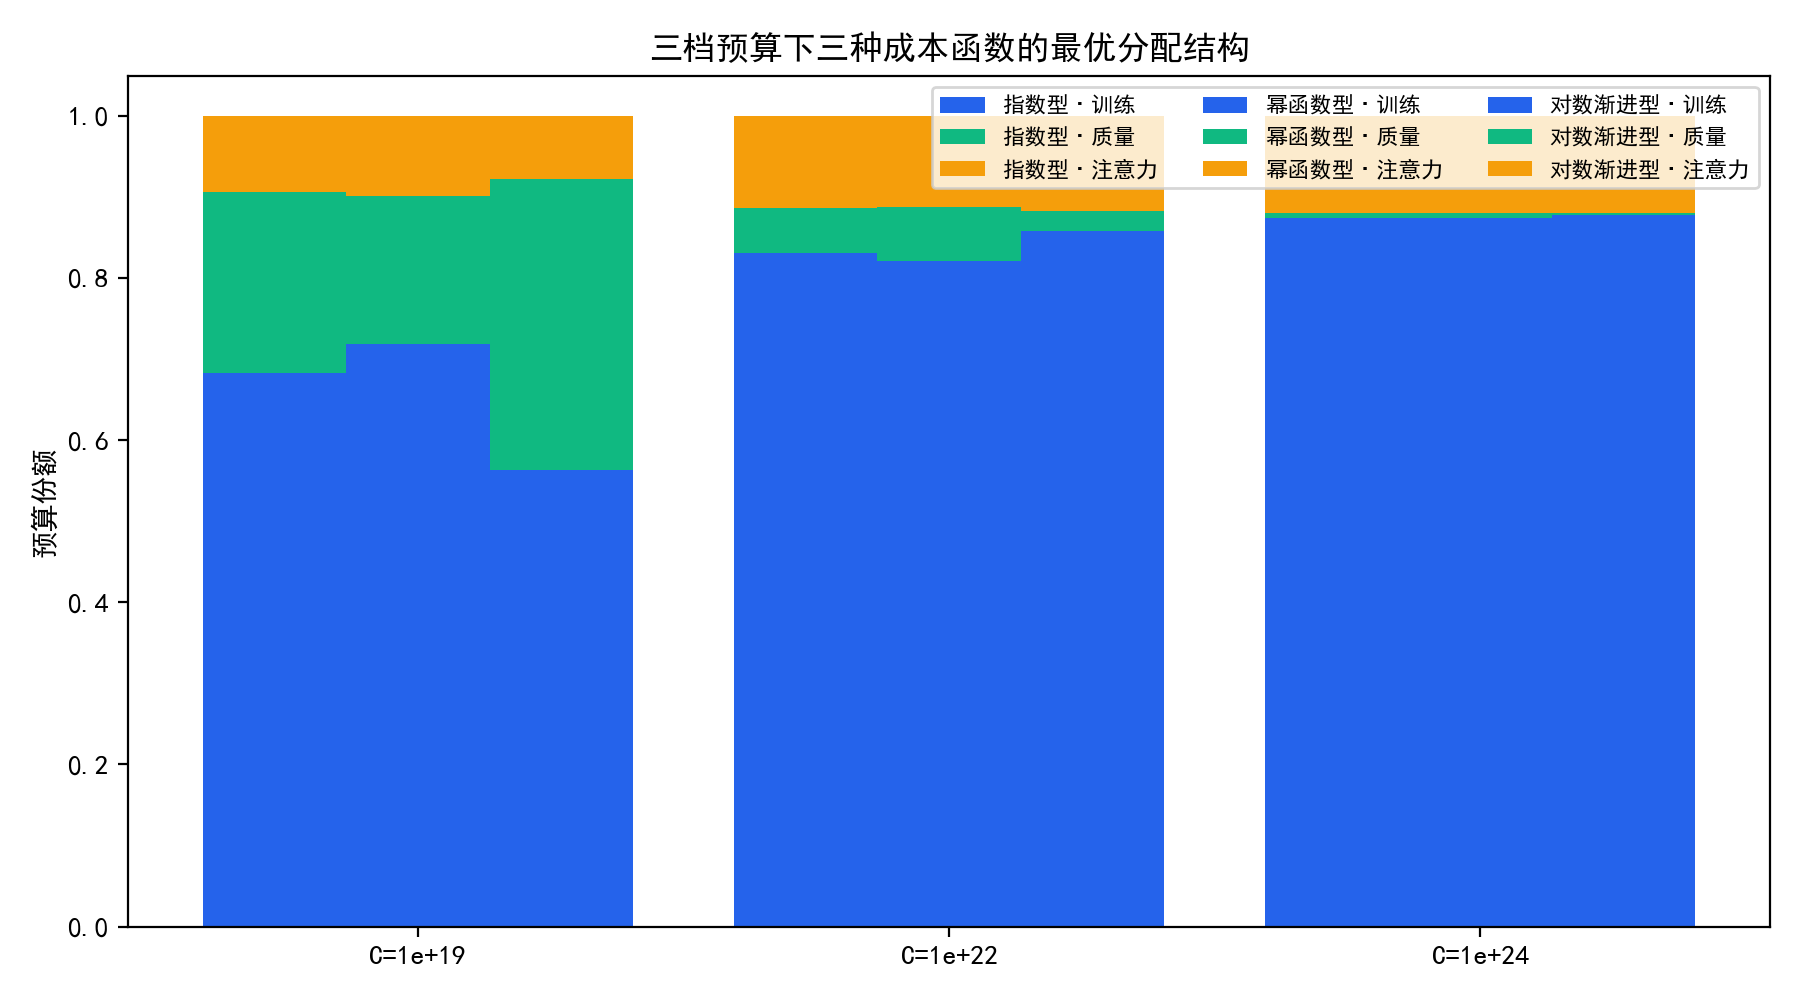
\includegraphics[width=0.9\textwidth]{figures/p3_budget_shares.png}
\caption{三档预算下三种质量成本函数的最优成本份额结构。}
\label{fig:p3_shares}
\end{figure}

\subsubsection{结构性转移点}

预算扫描识别的转移点（质量激活阈值）如下：

\begin{table}[htbp]
\centering
\caption{结构性转移点（$L_{\text{ctx}}=4096$）}
\begin{tabular}{c|ccc}
\toprule
成本函数 & 指数型 & 幂函数型 & 对数渐进型 \\
\midrule
$Q$ 激活阈值 $C^{*}$ & $6.3\times10^{17}$ & $2.0\times10^{18}$ & $3.2\times10^{18}$ \\
主导成本切换 & 无 & 无 & 训练$\leftrightarrow$质量（$3.2$--$5.0\times10^{18}$） \\
\bottomrule
\end{tabular}
\end{table}

三种成本函数下，$Q$ 离开基线 $Q_0$ 的预算阈值均落在 $10^{18}$ 量级（预算
低于阈值时最优策略为纯规模扩张、质量不投入；高于阈值时质量投入激活）。该
阈值可解析解释：质量激活条件为质量边际收益超过质量边际成本，前者
$\sim C(1-Q_0)^{g-1}N^{-h}$，后者 $\sim g'(Q_0)D$，两者交叉处即
$C^{*}$。三档预算中 $10^{19}$ 高于阈值、$10^{22}/10^{24}$ 远高于阈值，
故都呈现质量投入（前已述 $10^{22}$ 起 $Q^{*}=1$ 饱和）。对数渐进型成本在
$3.2\times10^{18}$--$5.0\times10^{18}$ 区间出现训练/质量主导的短暂切换，
这是其高 $Q$ 区增速放缓的直接体现；其余两型成本主导成分始终为训练——
结构性转移主要表现为\textbf{质量变量的边界--内点切换}。

\begin{figure}[htbp]
\centering
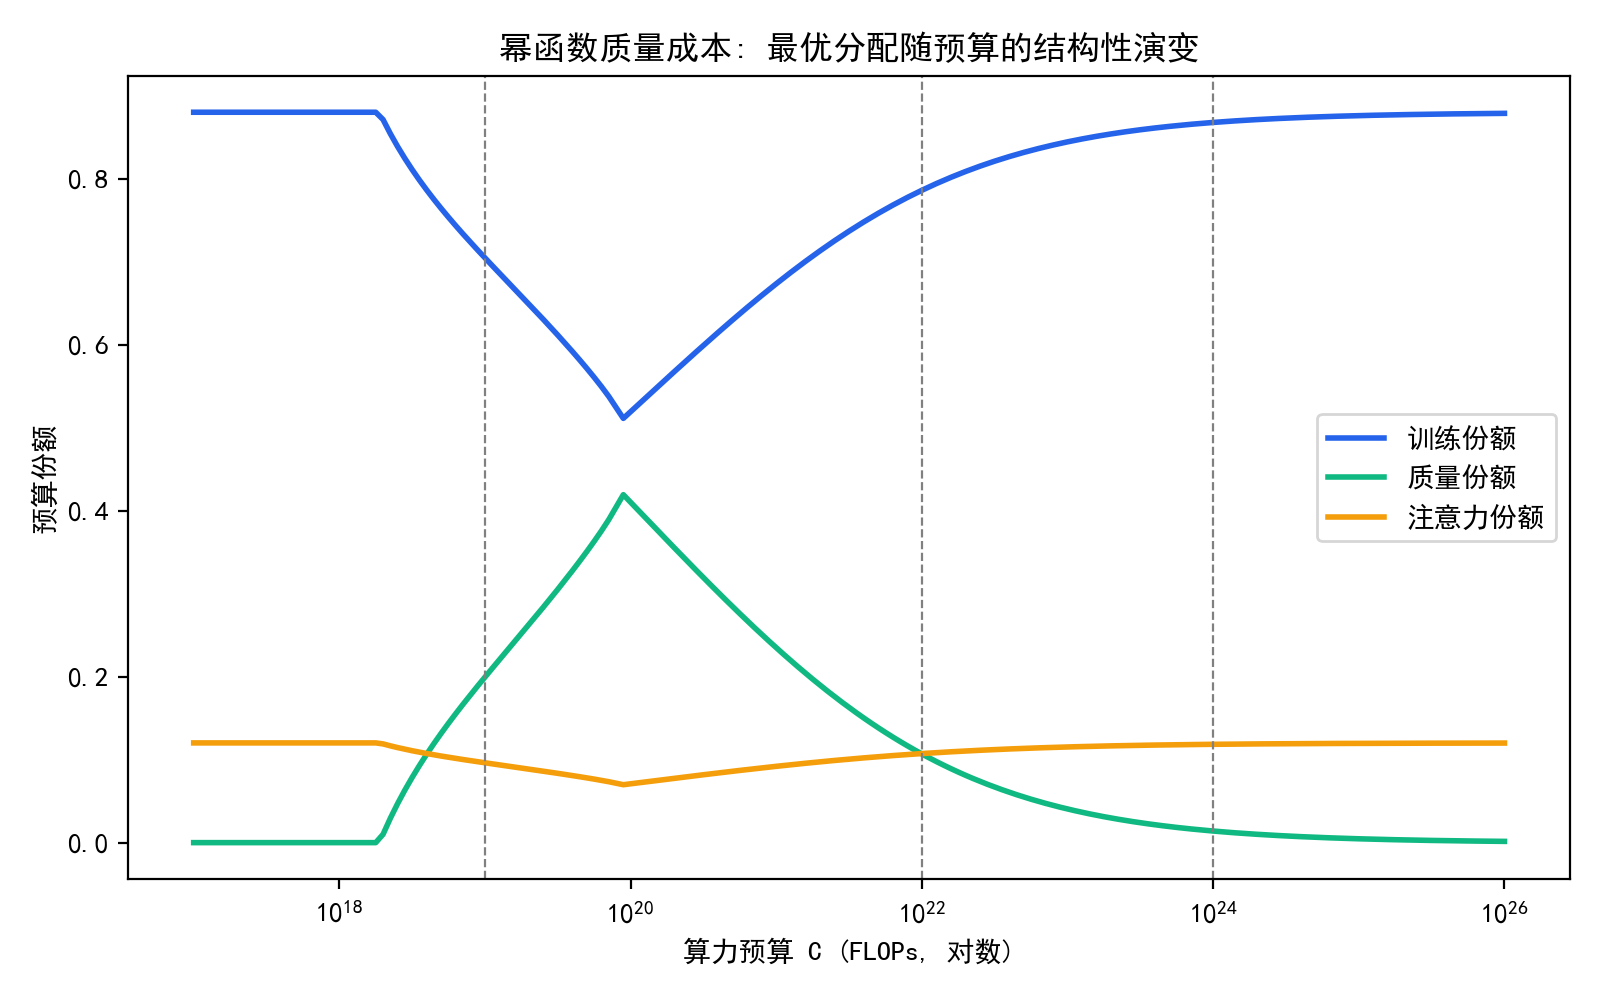
\includegraphics[width=0.85\textwidth]{figures/p3_structural.png}
\caption{幂函数质量成本下最优成本份额随预算的结构性演变（竖线为三档预算）。}
\label{fig:p3_structural}
\end{figure}

\subsubsection{$L_{\text{ctx}}$ 敏感性}

在 C7 可行值上扫描（幂函数质量成本）：

\begin{table}[htbp]
\centering
\caption{$L_{\text{ctx}}$ 敏感性（幂成本，$C=10^{19}$）}
\begin{tabular}{c|ccccc}
\toprule
$L_{\text{ctx}}$ & $N^{*}$(B) & $D^{*}$(B) & $Q^{*}$ & 训练份额 & 注意力份额 \\
\midrule
2048 & 0.307 & 4.08 & 0.591 & 0.752 & 0.051 \\
4096 & 0.298 & 3.94 & 0.597 & 0.704 & 0.096 \\
8192 & 0.282 & 3.69 & 0.608 & 0.625 & 0.171 \\
\textbf{30000} & \textbf{0.226} & \textbf{2.86} & \textbf{0.653} & \textbf{0.388} & \textbf{0.388} \\
32768 & 0.221 & 2.79 & 0.658 & 0.370 & 0.404 \\
131072 & 0.137 & 1.67 & 0.764 & 0.137 & 0.600 \\
\bottomrule
\end{tabular}
\end{table}

$L_{\text{ctx}}$ 越长，注意力份额越高、最优规模越小：$L_{\text{ctx}}$ 从
2048 增至 131072，$N^{*}$ 从 0.307B 降至 0.137B，$D^{*}$ 从 4.08B 降至
1.67B，损失从 3.24 升至 3.38（未列出）。在临界点 $L_{\text{ctx}}^{\text
{crit}}=30000$ 处注意力份额恰好等于训练份额（0.388 vs 0.388），与解析
结论 $\eta L_{\text{ctx}}/6=1$ 完全吻合，验证了数值求解的正确性。该结果
的政策含义：长上下文模型在相同预算下必须以缩小模型规模为代价，$10^{19}$
量级预算下 128k 上下文只能训练约 0.14B 参数的小模型。

\begin{figure}[htbp]
\centering
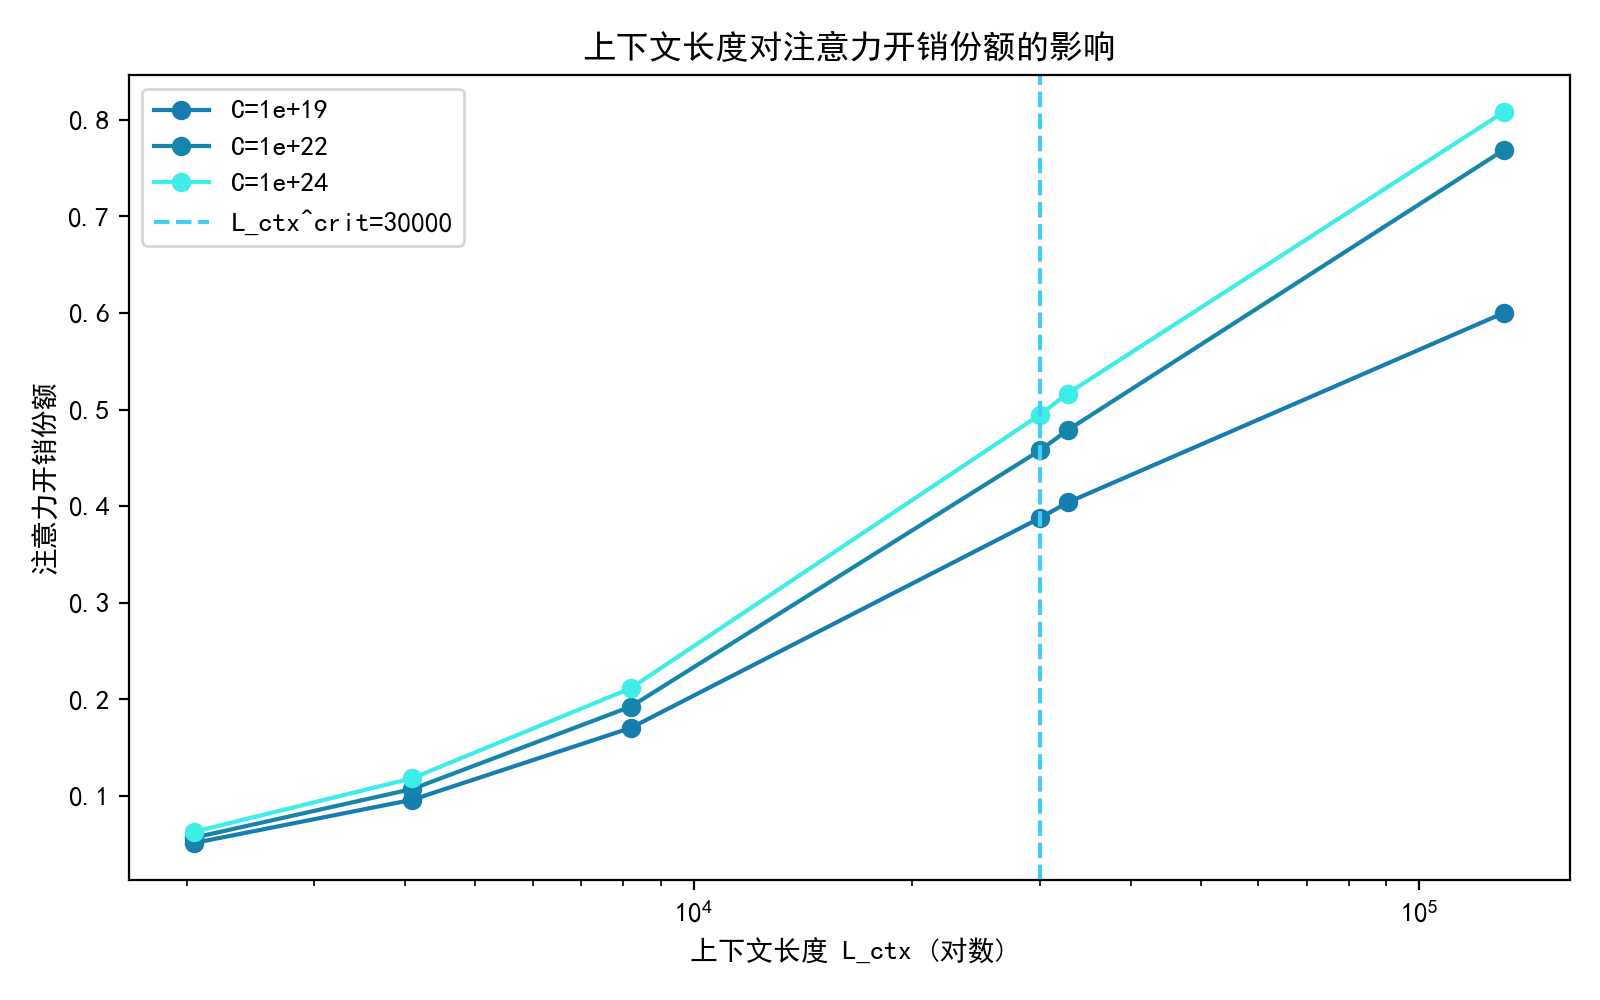
\includegraphics[width=0.85\textwidth]{figures/p3_lctx_sens.png}
\caption{注意力开销份额随上下文长度的变化（红色虚线为临界点 30000）。}
\label{fig:p3_lctx}
\end{figure}

\subsubsection{配比--质量--算力联合优化}

将问题一的 17 域语料配比向量 $p$ 引入作为第三层决策变量：质量由配比内生
决定 $Q=Q(p)=\sum_d p_d Q_d$（$Q_d$ 为问题一域级质量分），目标与约束同前。
该联合优化回答``在算力预算约束下，语料应如何配比''的问题。以 $C=10^{22}$
为例，最优解将配比几乎全部压向质量最高的小说域
（$Q_{\text{book}}=0.631$），$Q(p)$ 从均匀配比的 0.478 升至 0.631，损失
从 2.276 降至 2.238（改善约 2\%）；三档预算结论一致（$10^{19}$ 档小说域
占 74\%）。两类重要发现：

\begin{enumerate}
\item \textbf{配比优化的天花板}：$Q(p)$ 受最高质量域上限约束（此处
$Q_{\text{book}}=0.631$），仅靠重排配比无法达到 $Q=1$；配比优化带来的损失
改善（$\sim$2\%）远小于直接质量投资（$Q\to1$ 可再降损失至 2.148，改善
约 4\%）。这与弹性分析中``质量杠杆最有效''的结论一致，说明在质量维度上
\emph{直接改进数据本身比调整配比更重要}。
\item \textbf{数据配比现状偏离最优}：C 档实测配比的 $Q(p)=0.457$ 甚至低于
均匀配比（0.478），表明开源预训练语料的实际配比对质量维度几乎无偏置——这
为``数据配比存在优化空间''提供了定量证据。
\end{enumerate}

\begin{figure}[htbp]
\centering
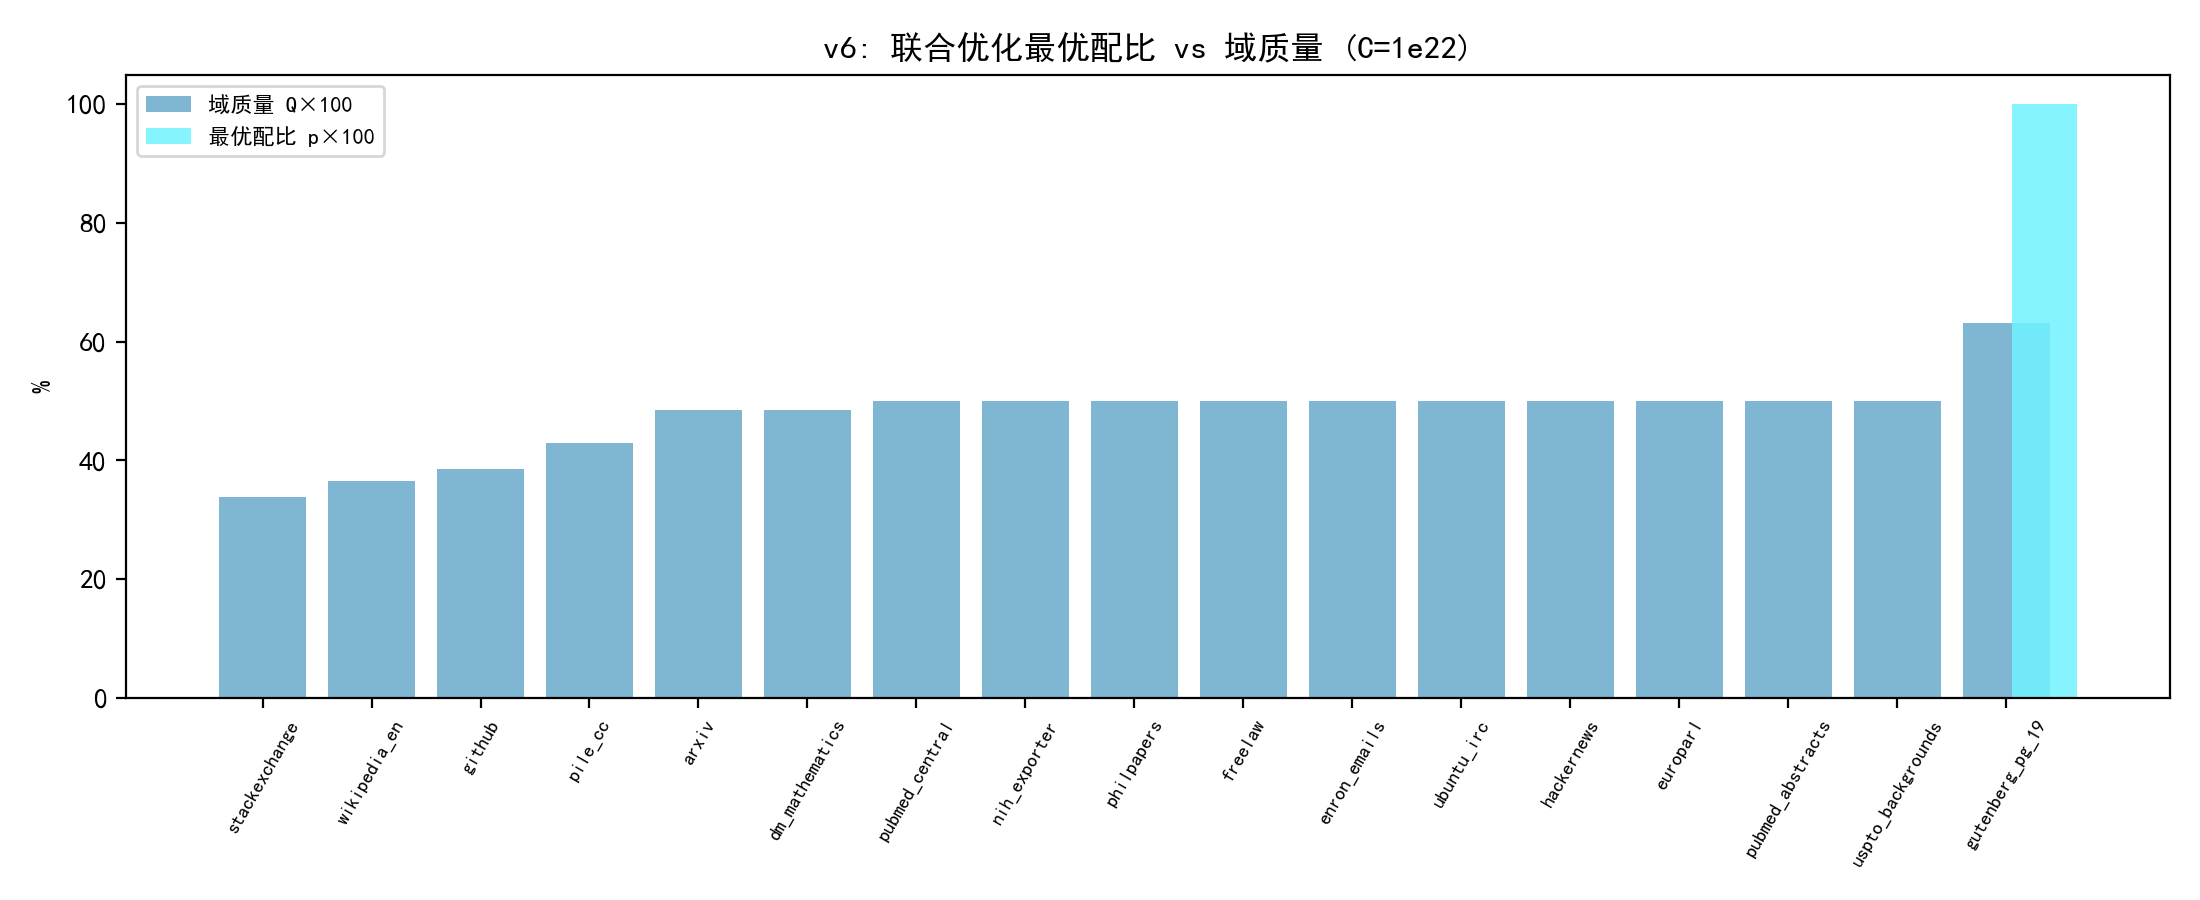
\includegraphics[width=0.9\textwidth]{figures/v6_p3_joint.png}
\caption{联合优化最优配比与域质量对比（$C=10^{22}$）：配比向最高质量域（小说）集中。}
\label{fig:p3_joint_mix}
\end{figure}

\subsubsection{上下文长度内生化}

前述优化将 $L_{\text{ctx}}$ 视为外生参数。本步将其提升为决策变量，并以
C7 架构元数据（40 个开源模型）拟合\textbf{上下文能力收益曲线}：
$\ln S=0.367+0.252\ln N+0.197\ln L_{\text{ctx}}$（$R^2=0.535$），即上下文
长度弹性 $0.197$（约等于参数量弹性的一半）。将收益项 $w\cdot
0.197\ln L_{\text{ctx}}$ 加入目标（$w$ 为收益权重）后联合优化：

\begin{itemize}
\item $w=0$（纯损失口径）：最优 $L_{\text{ctx}}$ 退到下限 512，与
``$L_{\text{ctx}}$ 越长损失越高''的结论一致；
\item $w=1$（实证收益口径）：$C=10^{22}$ 时最优 $L_{\text{ctx}}$ 直达架构
上限 131072（$w\ge0.5$ 时已饱和），注意力份额升至 77\%；
\item 权衡本质：长上下文以训练损失为代价换取能力收益——联合优化比固定
4096 的纯损失高 5.9\%，但总目标（损失减收益）更优。
\end{itemize}

\begin{figure}[htbp]
\centering
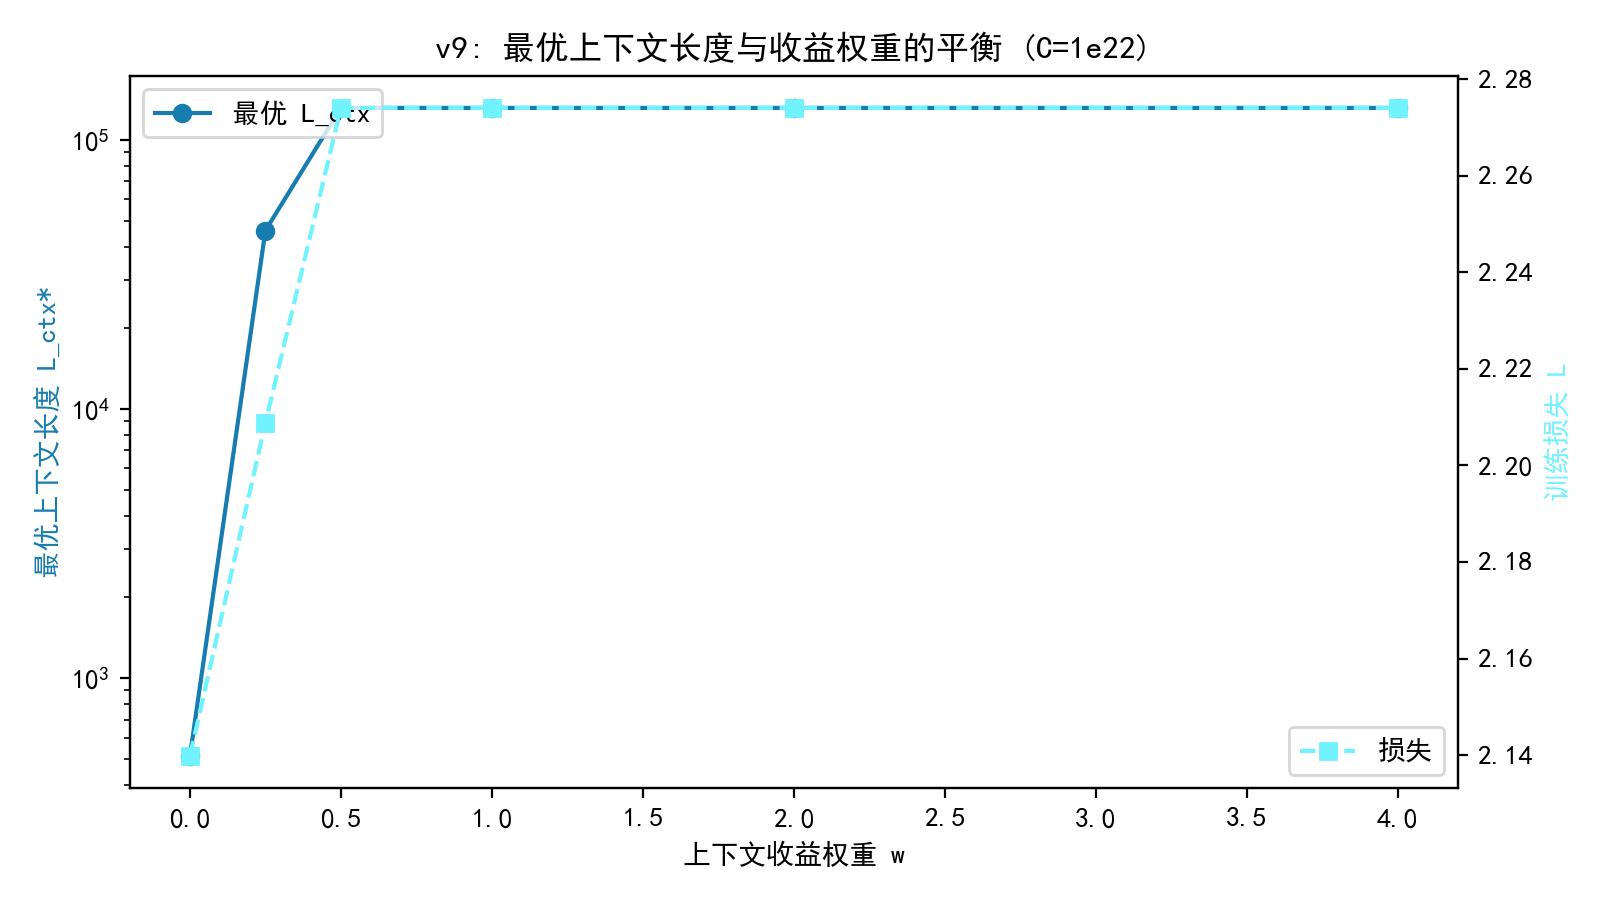
\includegraphics[width=0.8\textwidth]{figures/v9_p3_lctx_inner.png}
\caption{最优上下文长度与收益权重 $w$ 的平衡（$C=10^{22}$）。}
\label{fig:p3_lctx_inner}
\end{figure}

\subsection{小结}

问题三建立了三成本项联合优化模型，得到三档预算最优配置与结构性转移点：
$Q$ 激活阈值约 $10^{18}$ 量级（三种成本函数一致），$10^{22}$ 起质量饱和，
新增预算转向规模；$L_{\text{ctx}}$ 临界点 30000 的注意力--训练份额相等得到
数值验证。配比--质量--算力联合优化进一步表明：语料配比应向高质量域倾斜，
但配比杠杆有限（$\sim$2\%），直接质量投资才是主导途径。上下文长度内生化
（收益弹性 0.197 来自 C7 数据）显示：最优 $L_{\text{ctx}}$ 在纯损失口径下
取下限、在实证收益口径下取架构上限——上下文长度是``能力换损失''的权衡
决策，其最优值取决于收益权重。

\section{问题四的模型建立与求解}

按照``模型建立 $\to$ 模型求解 $\to$ 模型验证''的流程组织本节。问题四
要求：（1）基于附件 C 把开源模型能力提升分解为规模扩张与非规模技术
进步的贡献；（2）在算力增长放缓情景下预测未来 12/24 个月能力前沿并给不确定
区间；（3）完成至少一项基于 C8 的逐任务聚合分析。数据侧：C1/C2 为排行榜
（4576 条，6 维平均分 + 参数量 + 提交日期 + 许可证），C3 为扩展时序
（2019--2025），C4 为 Epoch 模型库（含算力、参数、开源权重标记），C5/C6
为 Loss--Benchmark 桥接，C7 为架构元数据，C8 为逐任务明细。

\subsection{模型建立}

\subsubsection{综合能力度量与数据口径}

\textbf{能力度量}：采用 C1 排行榜 6 维平均分 $S\in[0,100]$（IFEval、BBH、
MATH-Lvl5、GPQA、MUSR、MMLU-Pro 的平均）。该指标覆盖指令遵循、推理、数学、
科学问答与多步推理，作为综合能力代理变量。

\textbf{开源筛选口径}：以 C1 的 \texttt{Hub License} 含开源许可词
（apache/mit/bsd/llama/gemma/cc-by 等）为主判据，并交叉核对 C4 的
``Open model weights?'' 标记；筛选出开源模型 2496/4564 条，后续前沿分析
仅用开源子集，避免闭源模型（如 GPT 系列）的能力虚高与数据泄露。

\textbf{模型类型区分}：C1 的 \texttt{Type} 字段将模型分为 pretrained
（$n=275$）、chat/RLHF/DPO/IFT（$n=718$）、域特定微调（$n=1785$）与
基座合并（$n=1724$）等。按题意区分 pretrained 与 chat/finetuned，独立
复算（v80）：主链路全开源子集（$n=2493$）$b_N=0.364$、$b_T=0.089$、规模
贡献 83.7\%；\textbf{剔除 chat 与域微调子集}后（保留 pretrained/持续预训练/
基座合并等非对齐微调类型，$n=920$）$b_N=0.365$、$b_T=0.068$、规模贡献
升至 87.0\%——
``规模主导''对模型类型口径\textbf{稳健}；而纯 pretrained 子集（$n=239$，
样本稀疏）时间项 $b_T\approx-0.03$（年度趋势近似为零），chat 子集
（$n=459$）$b_T=0.129$——前沿分解中的``非规模技术''成分主要来自对齐/
微调通道的能力增益，纯预训练基座的年度技术进展有限。

\textbf{时间轴口径}：采用排行榜的\textbf{提交日期}（Submission Date）作为
时间轴——排行榜以提交即测为准，避免发布/版本日期在提交前多次迭代带来的
时间歧义（C4 的发布日期仅用于交叉核对开源权重标记）。

\textbf{开源子集对全量前沿的近似性核验}（图 \ref{fig:p4_opengap}）：按季度
对比开源前沿（开源行平均分最大值）与全量前沿：2024Q2 比值为 0.87，2024Q3
与 2025Q1 开源模型即为全量领跑者（比值 1.00），2024Q4 为 0.91——四个季度
中两个季度开源前沿\textbf{追平}全量前沿，平均比值约 0.95。开源子集作为
``前沿代表''的近似误差有限，且未系统性低估；这一核验也表明开源策略
（开放权重生态）在能力前沿上具备持续竞争力。

\begin{figure}[htbp]
\centering
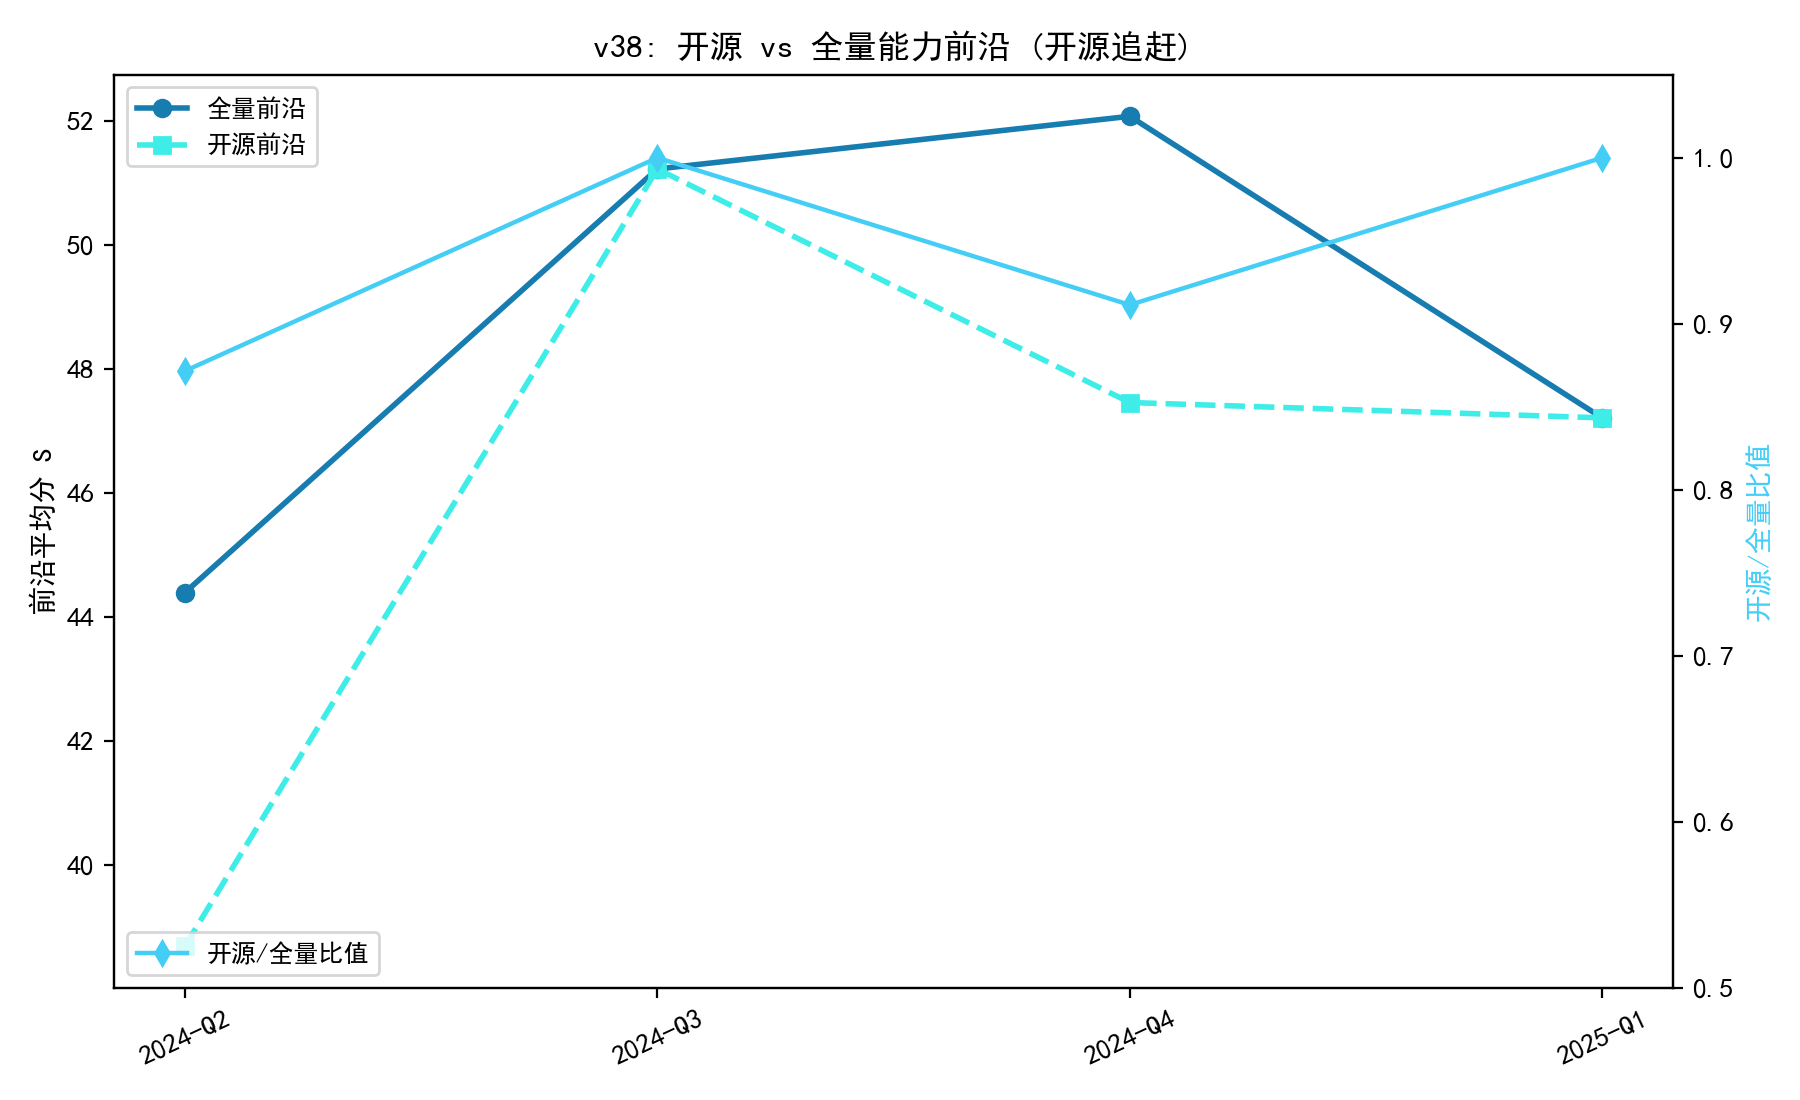
\includegraphics[width=0.82\textwidth]{figures/v38_p4_open_gap.png}
\caption{开源 vs 全量能力前沿：开源在 2024Q3/2025Q1 追平全量领跑。}
\label{fig:p4_opengap}
\end{figure}

\textbf{差距的规模段分解}（图 \ref{fig:p4_opeseg}）：把开/闭源差距按
参数规模分桶，中位分比值（open/closed）：$0.3$--$1$B 段 0.93$\to$0.89
（开源落后约 10\%）；$1$--$3$B 段 0.79$\to$1.13（\textbf{开源反超}）；
$3$--$10$B 段长期持平（约 1.00）；$10$--$30$B 段 1.35$\to$0.82$\to$1.07
（波动后趋平）；$30$--$100$B 段 0.88$\to$0.98（追赶中，样本较稀）。
\textbf{开源追赶分规模段}：中段（$1$--$10$B）已基本完成/接近，两端
（最小端与头部大模型）仍落后约 10\%——v38 的平均比值 0.95 在此分解为
``中段持平 + 两端滞后''的结构。

\begin{figure}[htbp]
\centering
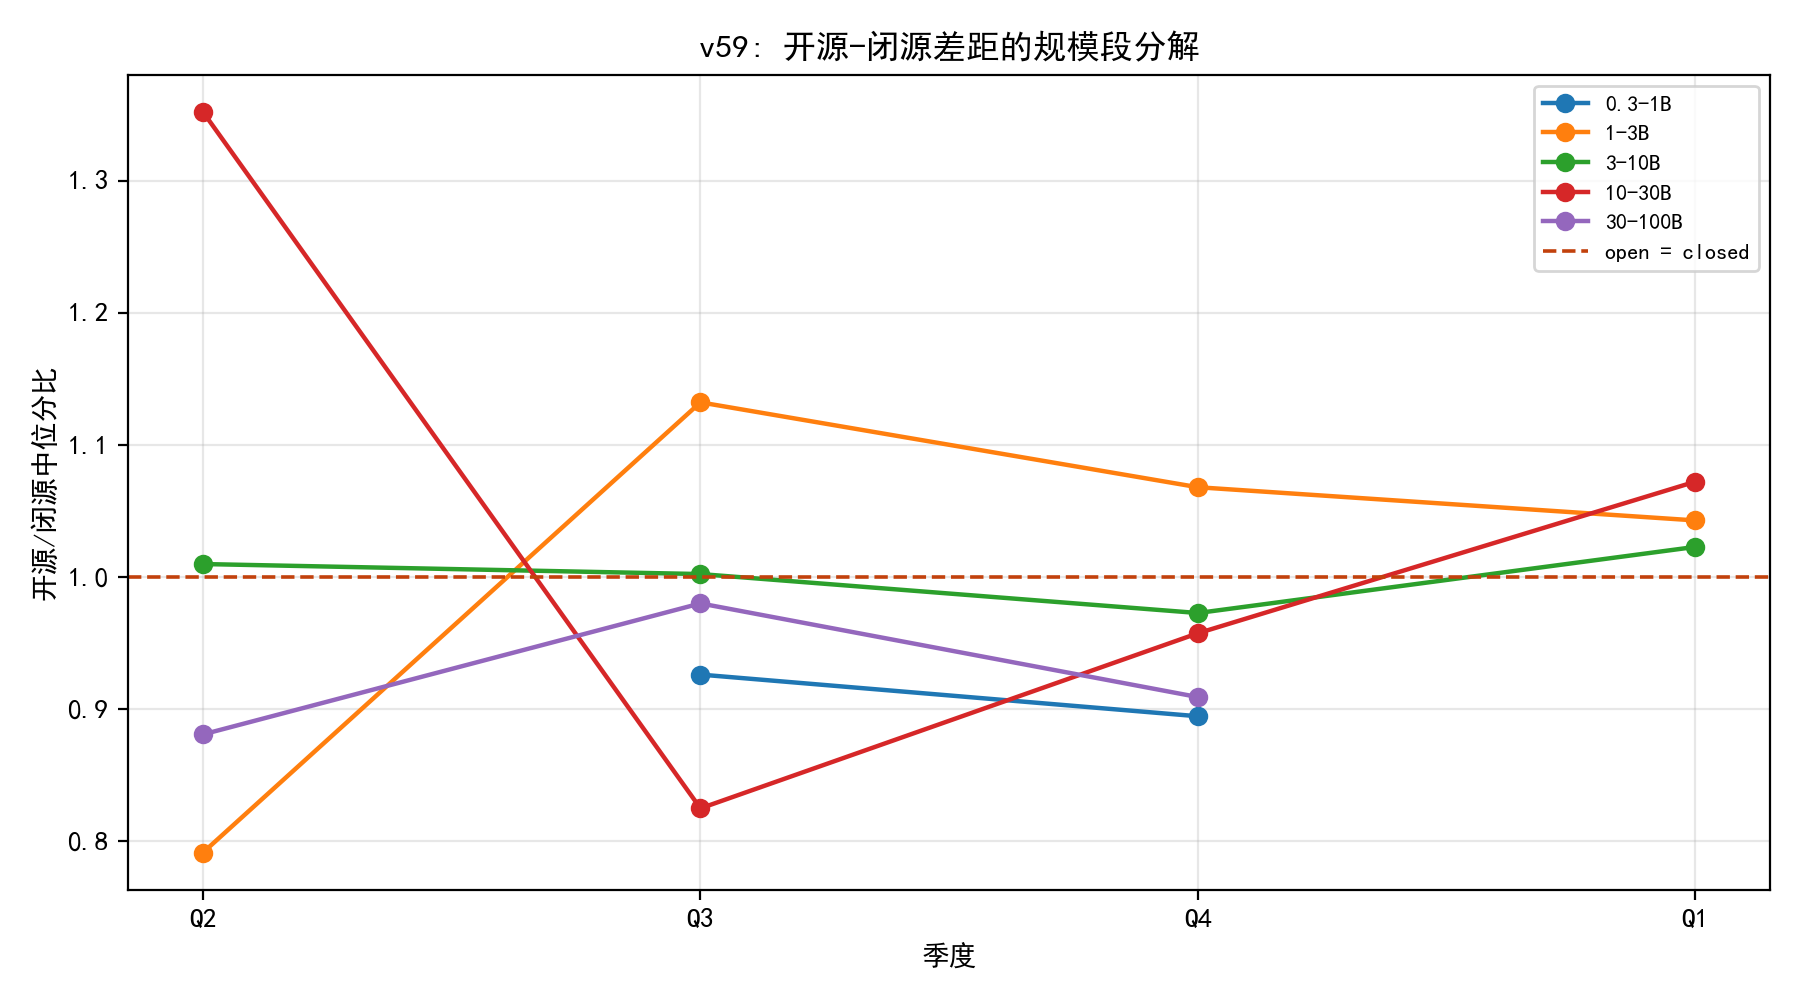
\includegraphics[width=0.85\textwidth]{figures/v59_p4_open_seg.png}
\caption{开源--闭源差距的规模段分解：中段持平、两端滞后约 10\%。}
\label{fig:p4_opeseg}
\end{figure}

\textbf{开源前沿的家族竞争动态}（图 \ref{fig:p4_family}）：按季度识别开源
领跑家族：2024Q2 为 Llama（38.7），Q3 与 2025Q1 由其他家族领跑（51.2/47.2，
Qwen 连续居于次席），Q4 为 Qwen（47.5）。前 5 高分模型家族的 HHI 从 2024Q2
的 1.00（单家垄断）降至 Q3--Q4 的 0.52、2025Q1 的 0.68，季度内活跃家族数
9--11——开源前沿的竞争从``一家独大''走向``多家族并立''，且 Qwen 持续
占据领跑梯队，家族更替快于单一模型的换代周期。

\begin{figure}[htbp]
\centering
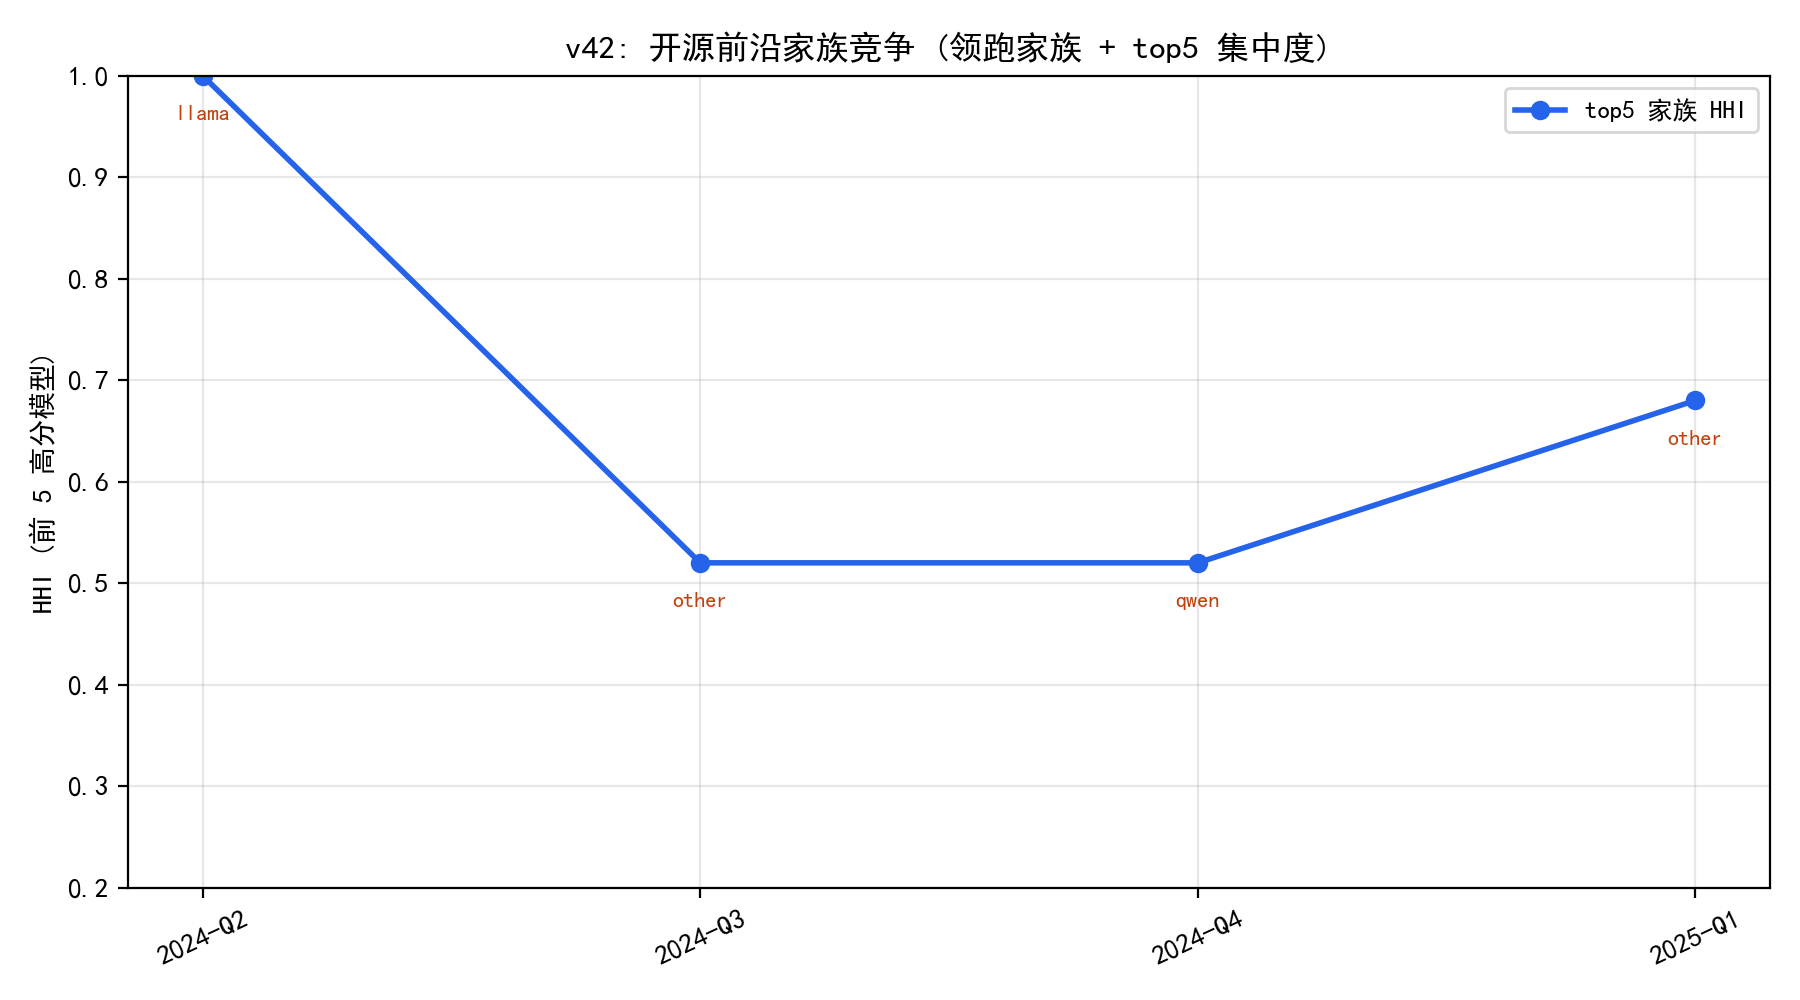
\includegraphics[width=0.8\textwidth]{figures/v42_p4_family_dyn.png}
\caption{开源前沿家族竞争：领跑家族轮替与 top5 集中度（HHI）。}
\label{fig:p4_family}
\end{figure}

\textbf{追赶时间的外推预测}（图 \ref{fig:p4_catchup}）：v42 给出的是
\textbf{历史轮替}（领跑身份季度间更迭），这里用 2025-03 家族 90 分位与
对数线性增速做\textbf{前向外推}：领跑者为 Qwen（43.1，月增速 +0.057）；
仅 ``other'' 聚合类（41.9，差距 3\%）预计约 6 个月追平、Mistral（38.1）
需约 137 个月（11 年，仅略快）；Phi（39.9）、Gemma（21.6）增速不足，
\textbf{Llama（30.5）月增速仅 +0.004（年化 +0.04，近乎停滞）}、Yi
（12.7）甚至负增长（$-1.39$/年），均判定为``永不''收敛（当前增速差
持续）。合起来：近期多强轮替（v42），\textbf{外推下收敛到 Qwen 单极 +
其余固定差距}——增速结构比领跑身份更能预示格局走向。（注意：90 分位
增速含发布节奏噪声，``永不''指当前增速差延续的推演；对增速结构做
模型层 Bootstrap（300 次）后，确定性外推中可追赶的 other/Mistral 两族
``永不收敛''的样本占比仍达 53\%--65\%，追赶时间 90\% 区间分别宽达
$1.1$--$63.9$、$4.4$--$213.5$ 个月——外推不确定性显著，结论仅在增速
结构维持假设下成立。）

\begin{figure}[htbp]
\centering
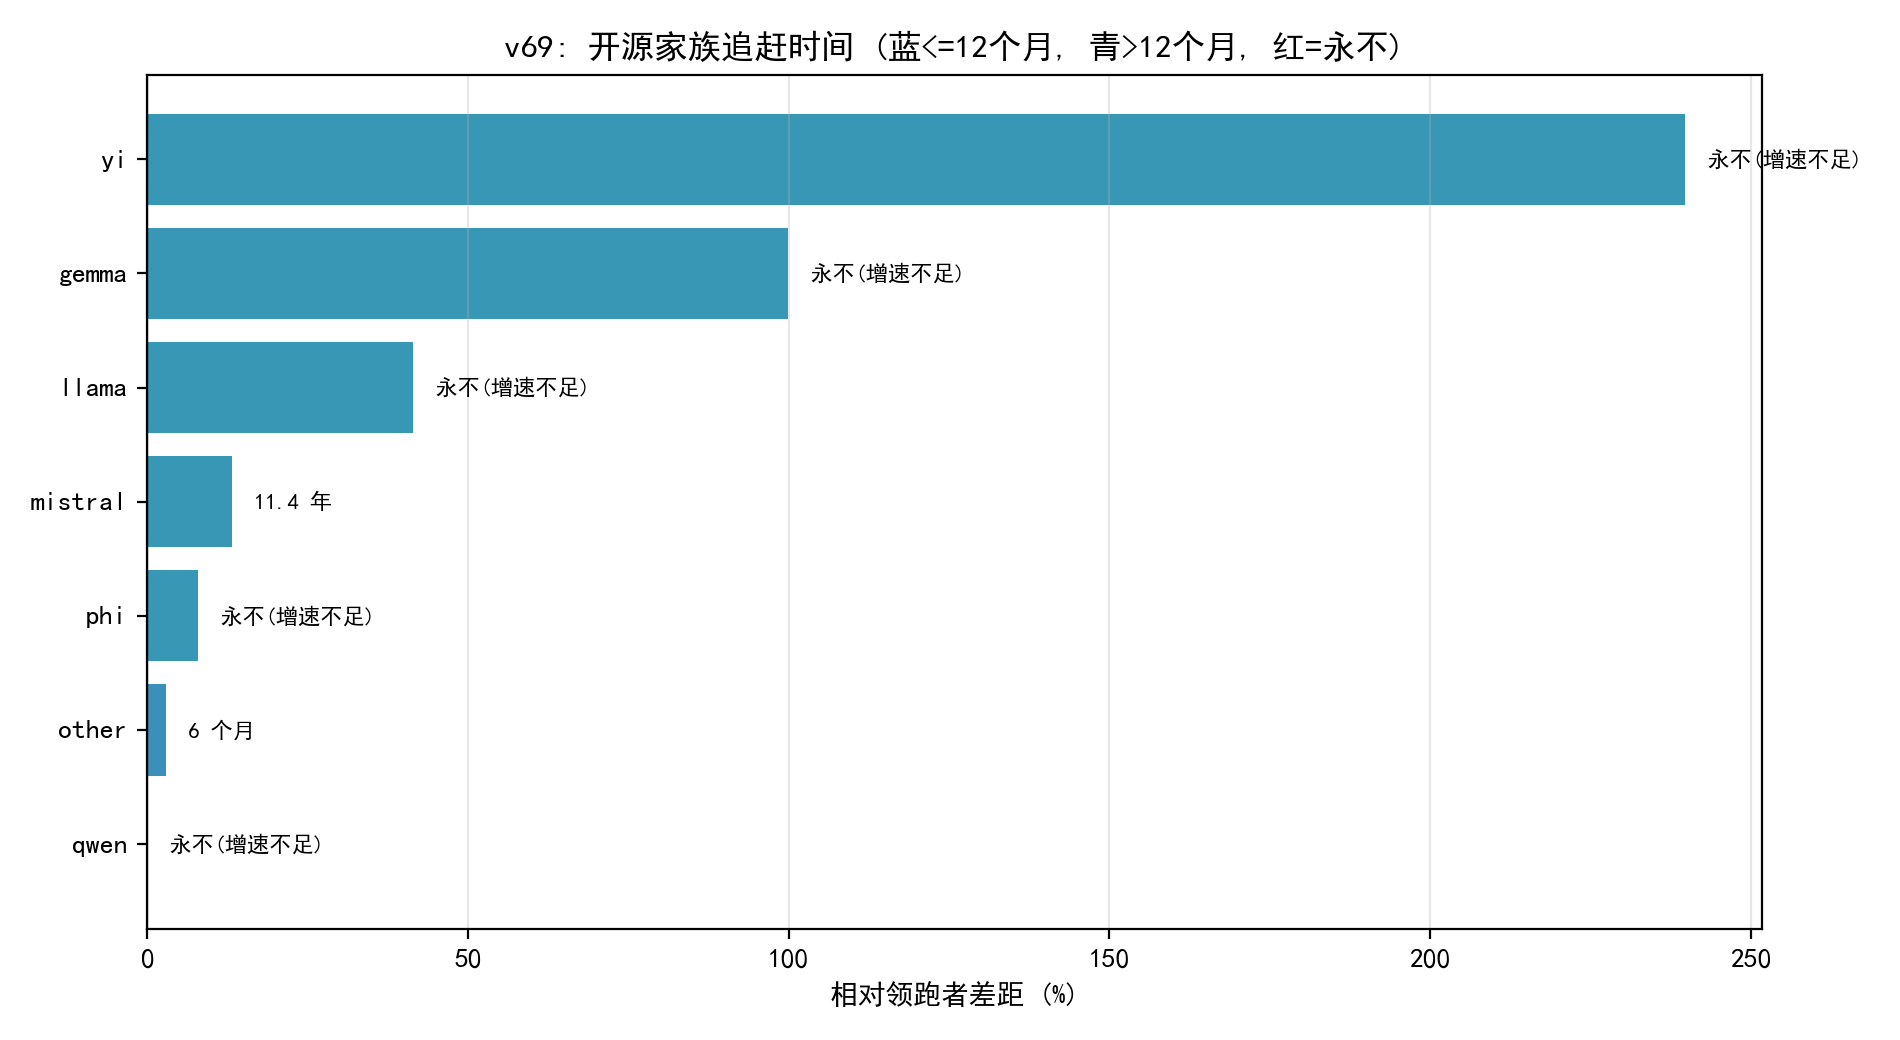
\includegraphics[width=0.85\textwidth]{figures/v69_p4_catchup.png}
\caption{家族追赶时间：仅 other 可短期追平，Llama 近乎停滞。}
\label{fig:p4_catchup}
\end{figure}

\textbf{时间轴口径}：以 C1 的提交日期（Submission Date）作为年份依据；
C3 的历史前沿（2019--2021）作为补充背景，取累计最大值以保证前沿单调不降
（2020 年出现 50.0 的孤立高值、2021 回落，属半合成扩展数据，取累计口径
规避该噪声）。

\subsubsection{前沿能力模型}

对开源模型样本建立 90\% 分位数回归：
\begin{equation}
\ln S = c + b_N \ln N + b_T t,
\label{eq:frontier}
\end{equation}
其中 $t$ 为以 2022 年为 0 的年份。分位数回归（线性规划形式，Koenker--
Bassett 精确解）对前沿点稳健，比均值回归更能刻画``能力前沿''。拟合结果
（$n=2493$）：
\begin{equation}
c=2.481,\qquad b_N=0.364,\qquad b_T=0.089.
\label{eq:frontier_fit}
\end{equation}
解释：$b_N=0.364$ 表示参数每翻倍、前沿平均分（对数尺度）提升
$\ln2\times0.364\approx0.252$，对应水平增幅约 $28.7\%$；$b_T=0.089$
表示即使参数不变，每年前沿
整体上移约 9\%——这就是非规模技术进步（算法、对齐、数据组织、工程优化）的
量化体现。作为对照，普通最小二乘会得到 $b_T=0.20$（高估技术增速），
Huber 稳健回归 $b_T=0.24$（v79 复算），均因受大量非前沿样本拖累而失真；分位数回归
专门追踪前沿点，取值最可信。对参数做 300 次样本自助（在 $\tau=0.9$ 的
线性规划分位数回归上重抽）得 90\% 置信区间：$b_N\in[0.347,0.378]$、
$b_T\in[0.068,0.103]$，均显著异于 0；对应规模贡献占比区间约为
81\%--87\%，``规模主导''结论在参数不确定性下稳健。

\textbf{跨框架一致性核验}（图 \ref{fig:p4_qrfw}）：为保证分位数前沿结论
不依赖统计实现，用五个相互独立的框架复算同一 $\tau=0.9$ 回归——线性规划
精确解（HiGHS，主链路）、statsmodels QuantReg、sklearn
QuantileRegressor（$\alpha=0$）、L-BFGS-B 直接极小化 pinball 损失与 Adam
梯度下降。结果：\textbf{五框架复现同一系数}——$c_0=2.481$、$b_N=0.364$、
$b_T=0.089$（相对极差：$c_0$ 为 $4\times10^{-3}\%$、$b_N$ 为
$2\times10^{-2}\%$、$b_T$ 为 $3\times10^{-1}\%$——后者来自 Adam 梯度下降
在有限步数下的微小未收敛，其余四框架逐位一致），pinball 目标值在
LP/statsmodels/sklearn/L-BFGS-B 四框架一致到 6 位小数（135.95035；
Adam 相差 $\le2\times10^{-3}$），$n=2493$ 个样本上的预测最大跨框架差异
仅 $1.0\times10^{-3}$。代入
增长核算式 (\ref{eq:growthacc})（$g_N=1.251$），五个框架给出的规模贡献
占比\textbf{全部为 $83.66\%$}（差异 $\le4\times10^{-4}$）。跨
scipy/statsmodels/sklearn/torch 四个统计生态的独立实现收敛到同一前沿，
证明\textbf{前沿系数与规模/非规模分解对估计器实现数值稳健}。

\begin{figure}[htbp]
\centering
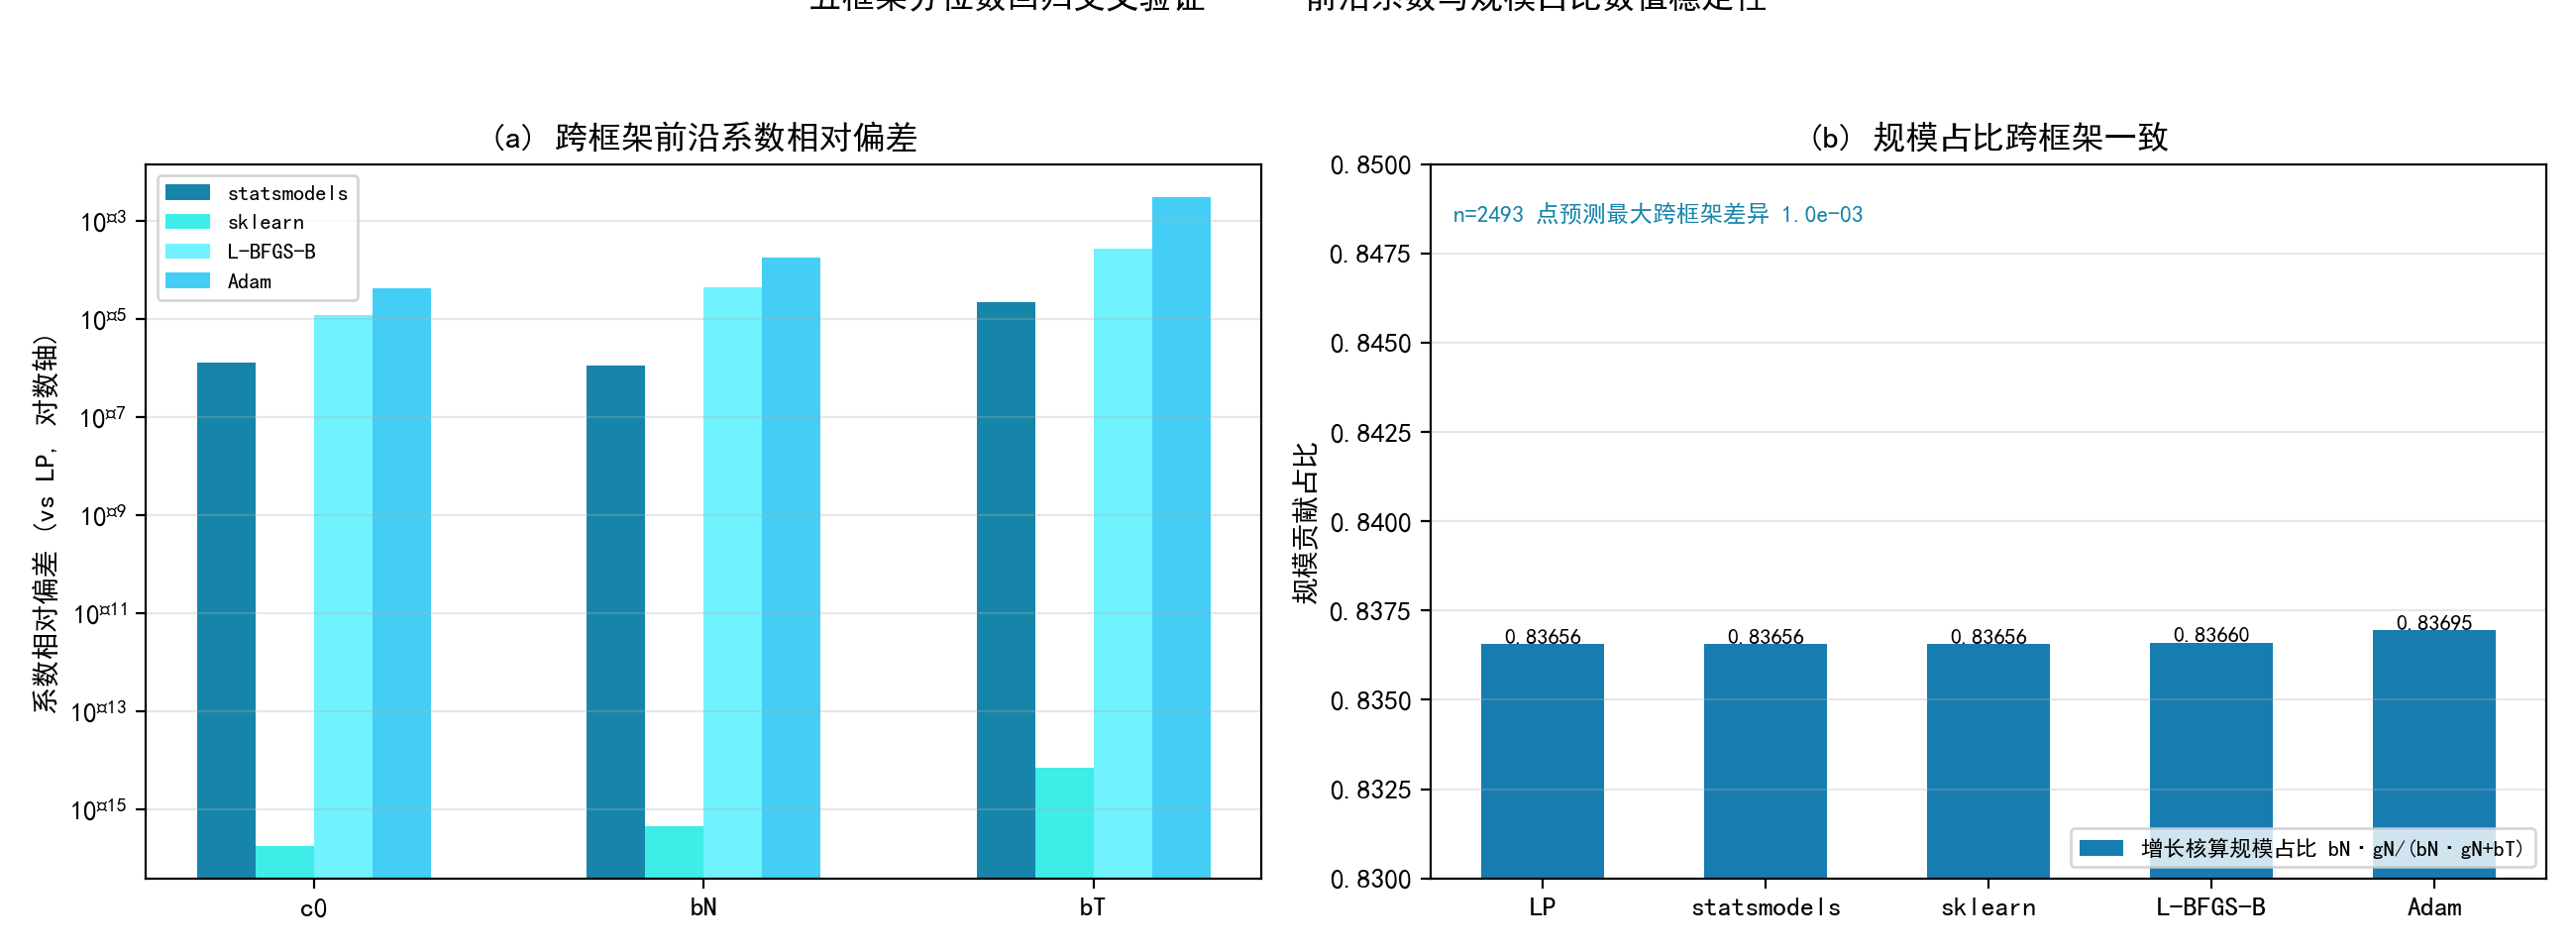
\includegraphics[width=0.95\textwidth]{figures/v74_p4_qr_frameworks.png}
\caption{五框架分位数回归交叉验证：系数与规模贡献占比（83.7\%）跨框架一致。}
\label{fig:p4_qrfw}
\end{figure}

\begin{sloppypar}%
\textbf{分位数族一致性}（图 \ref{fig:p4_taurange}）：将五框架交叉验证扩展到
分位数族 $\tau\in\{0.5,0.7,0.8,0.9,0.95,0.99\}$。结果：\textbf{框架无关性
在整族成立}——每个 $\tau$ 上五框架系数最大相对极差
$b_N\le1.3\times10^{-1}\%$、$b_T\le1.9\%$（后者主要来自 Adam 在 $\tau=0.99$
的有限步数未收敛；剔除 Adam 后，LP/statsmodels/sklearn/L-BFGS-B 四框架在
每个 $\tau$ 上高度一致，$b_N$ 极差 $\le1.2\times10^{-4}$、$b_T$ 极差
$\le0.6\%$）。系数随 $\tau$ 的结构具有明确含义：
\end{sloppypar}
\begin{itemize}
\item $b_T$ 自 $\tau\ge0.8$ 起\textbf{单调递减}（$0.177\to0.089\to0.044$；
$\tau=0.5/0.7$ 更高，为 $0.248$）：
分位越低、时间趋势越强——中分位模型主要以时间追赶，而 0.9 分位前沿的进步
更依赖规模扩张（$b_N=0.364$），0.99 分位的时间趋势趋近于 0（$0.044$），
顶级模型的进步几乎完全由规模驱动；
\item $b_N$ 在 $\tau\le0.8$ 缓升（$0.366\to0.372$）后\textbf{回落}
（$0.340\to0.279$）：极端尾部（0.95/0.99）的规模回报趋于饱和，参数弹性
下降，与问题四``前沿能力向硬推理迁移、大桶能力饱和''的任务侧观测互证；
\item $\tau=0.9$ 的选取位于 $b_T$ 单调递减的稳健中段、$b_N$ 峰后回落之前，
\textbf{非极端选取}；代入增长核算后，规模贡献占比随 $\tau$ \textbf{单调
上升}：$64.9\%\to65.0\%\to72.5\%\to83.7\%\to85.4\%\to88.8\%$
（$\tau=0.5$--$0.99$）——分位越高、时间趋势越小，前沿越由规模驱动；
``规模主导''在 $\tau\ge0.8$ 的整个前沿区间（占比 $\ge72.5\%$）恒成立且
单调递增。
\end{itemize}

\begin{figure}[htbp]
\centering
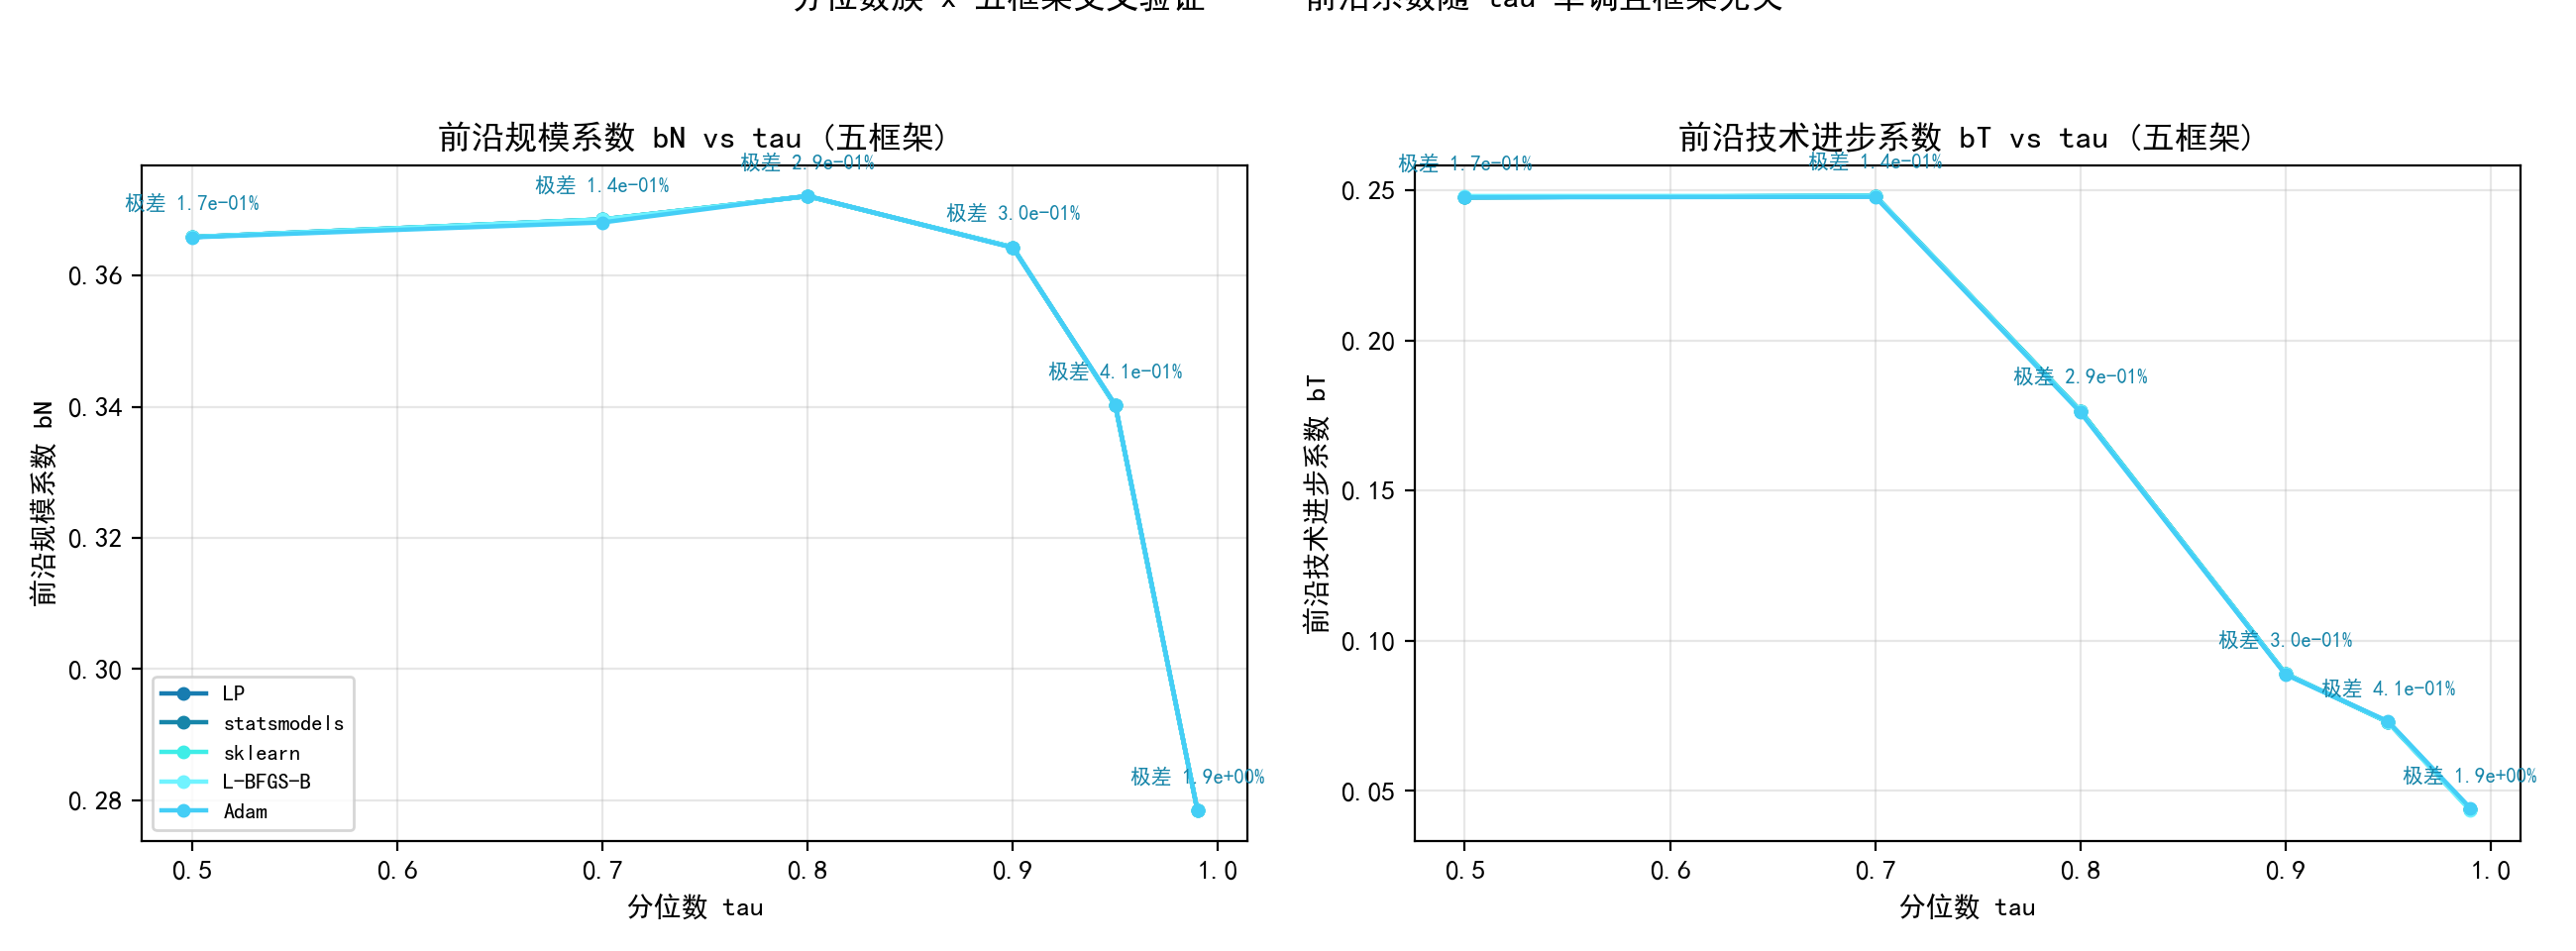
\includegraphics[width=0.95\textwidth]{figures/v77_p4_tau_frameworks.png}
\caption{分位数族 $\times$ 五框架：每个 $\tau$ 上五框架一致；$b_T$ 随 $\tau$
单调递减、$b_N$ 峰后回落。}
\label{fig:p4_taurange}
\end{figure}

\subsection{模型求解}

\paragraph{规模/非规模贡献分解}

\textbf{增长核算}：前沿能力的年增速可分解为：
\begin{equation}
\frac{d\ln S}{dt}=\underbrace{b_N g_N}_{\text{规模贡献}}
+\underbrace{b_T}_{\text{非规模技术贡献}},
\label{eq:growthacc}
\end{equation}
其中 $g_N=d\ln N/dt$ 为开源模型参数量对数年增速。由 C4 开源模型按年份
90\% 分位参数量拟合 $\ln N=\text{const}+g_N t$ 得 $g_N=1.251$（约为每年
3.5 倍）。代入得：
\begin{equation}
\text{规模贡献}=b_N g_N=0.456\ (83.7\%),\qquad
\text{非规模技术贡献}=b_T=0.089\ (16.3\%).
\label{eq:decomp}
\end{equation}
结论：过去数年开源模型前沿能力的提升约 84\% 来自规模扩张（更大参数量），
约 16\% 来自非规模技术进步。这一分解表明，即便算力增长放缓（参数量增速
减半），非规模技术进步仍能维持约 0.089/年的底线增速——这是预测情景构建的
关键。

\paragraph{前沿预测（12/24 个月）}

\paragraph{情景设定}

\begin{itemize}
\item \textbf{基准点}：2025 年分位数前沿水平 $\hat S_{2025}=41.6$（对应
90\% 分位参数约 14.7B，$\ln N=2.69$），由 \eqref{eq:frontier_fit} 代入
$t=3$ 得到；
\item \textbf{基础情景}：参数量增速延续历史 $g_N=1.251$；
\item \textbf{算力放缓情景}：参数量增速减半 $g_N=0.626$（模拟算力供给
受限、摩尔定律放缓）；
\item \textbf{不确定性}：对前沿外推噪声（$\sigma=0.12$，由残差标准差
校准）自助采样 800 次，取 10\%/90\% 分位为置信区间。
\end{itemize}

\paragraph{预测结果}

\begin{table}[htbp]
\centering
\caption{开源模型能力前沿预测（$S$：6 维平均分）}
\begin{tabular}{c|c|cc|cc}
\toprule
 & & \multicolumn{2}{c|}{基础情景} & \multicolumn{2}{c}{算力放缓情景} \\
时间 & 预测中位 & 90\% 区间 & & 90\% 区间 \\
\midrule
2026.0（12 个月） & 71.7 & [61.5, 83.4] & 57.1 & [48.4, 66.7] \\
2027.0（24 个月） & 123.9 & [105.0, 142.3] & 78.6 & [67.7, 92.3] \\
\bottomrule
\end{tabular}
\end{table}

基础情景下 12 个月前沿平均分约从 41.6 升至 71.7（+72\%）、24 个月升至
123.9（+198\%）；放缓情景下分别为 57.1（+37\%）与 78.6（+89\%）。放缓
情景与基础情景的差距随预测期扩大：24 个月时放缓情景比基础情景低约 45 分，
凸显算力供给对前沿演进速度的显著约束。两个情景的 90\% 区间随预测期变宽，
反映了外推不确定性的累积（且双情景区间涵盖备选趋势形式的投影，见下文的
趋势形式回测对比）。

\textbf{预测不确定性的来源分解}（图 \ref{fig:p4_uncert}）：用全方差定律
把预测区间方差分解为三个来源——残差 $\varepsilon$（报告 CI 校准
$\sigma=0.12$）、参数不确定性（$b_N,b_T,c$ 的 Bootstrap 区间）、增速假设
$g_N$ 情景（$0.4$--$1.6$）。12 个月：残差 42.6\%、参数 11.8\%、$g_N$
46.1\%；24 个月：残差 17.2\%、参数 7.3\%、$g_N$ \textbf{77.6\%}——
\textbf{$g_N$ 情景是长周期预测不确定性的主导来源}，其贡献随预测期扩大
（$\ln N$ 增长项 $g_N h/12$ 的放大效应），与 $g_N$ 敏感性分析的
$\pm75\%$（24 个月）互证；残差在 12 个月口径下与 $g_N$ 相当，参数
不确定性全程可忽略（约 7--12\%）。若改用全样本 QR90 原始残差
（$\sigma=0.481$），残差占比升至 78\%--92\%——残差份额依赖校准口径，
但\textbf{$g_N$ 主导长周期不确定性的定性结论在两种口径下均成立}。

\begin{figure}[htbp]
\centering
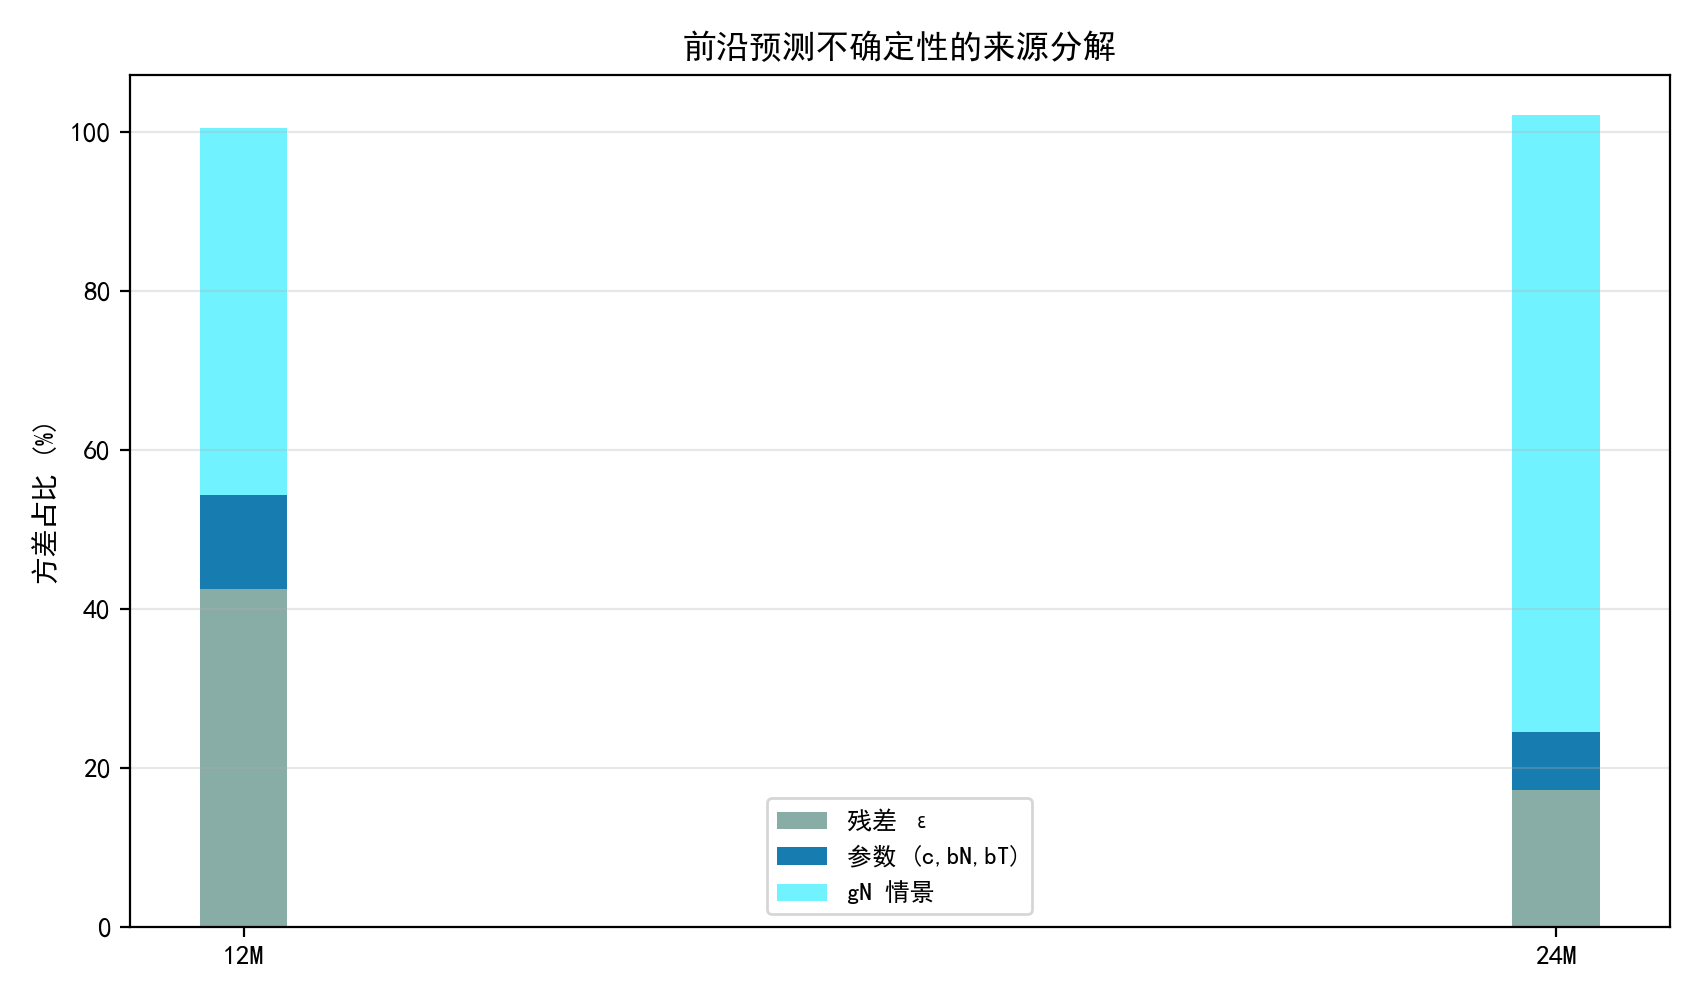
\includegraphics[width=0.8\textwidth]{figures/v54_p4_uncert_budget.png}
\caption{前沿预测不确定性的来源分解（12M/24M）。}
\label{fig:p4_uncert}
\end{figure}

\textbf{能力目标的算力落地换算}（图 \ref{fig:p4_computeconv}）：把 P4 的
前沿模型（QR90 反解 $N$）与 v24 的数据最优曲线（$D^{*}(N)=49.8N^{1.046}$）
串成``能力目标 $\to$ 训练算力 $\to$ 工程规模''的决策换算器（2025 年，
整数年口径）：$S=70$ 需 $N\approx62$B、$1.4\times10^{24}$ FLOP（H100
$\approx1.6$ 万卡天）；$S=90$ 需 123B、$5.7\times10^{24}$（$\approx6.6$
万卡天）；$S=120$ 需 271B、$2.8\times10^{25}$（$\approx33$ 万卡天）；
$S=150$ 需 501B、$1.0\times10^{26}$（$\approx116$ 万卡天）——$S$ 从
60 到 150 跨越约 2.2 个数量级。作为对照，P3 联合优化在 $C=10^{22}$ 预算
下（幂型中位解 $N^{*}\approx6.1$B、$D^{*}\approx238$B）按 $6ND$ 规则的
训练算力约 $8.8\times10^{21}$ FLOP。
\textbf{说明}：$D^{*}$ 曲线为理论最优（数据充足假设），$C_{train}$ 不含
质量/注意力成本，H100 取理想吞吐，因此本表给出的是\textbf{下界量级}而非
精确预算；其价值在于把 P2 标度律、P3 优化、P4 预测串联为可直接使用的
预算决策接口。

\begin{figure}[htbp]
\centering
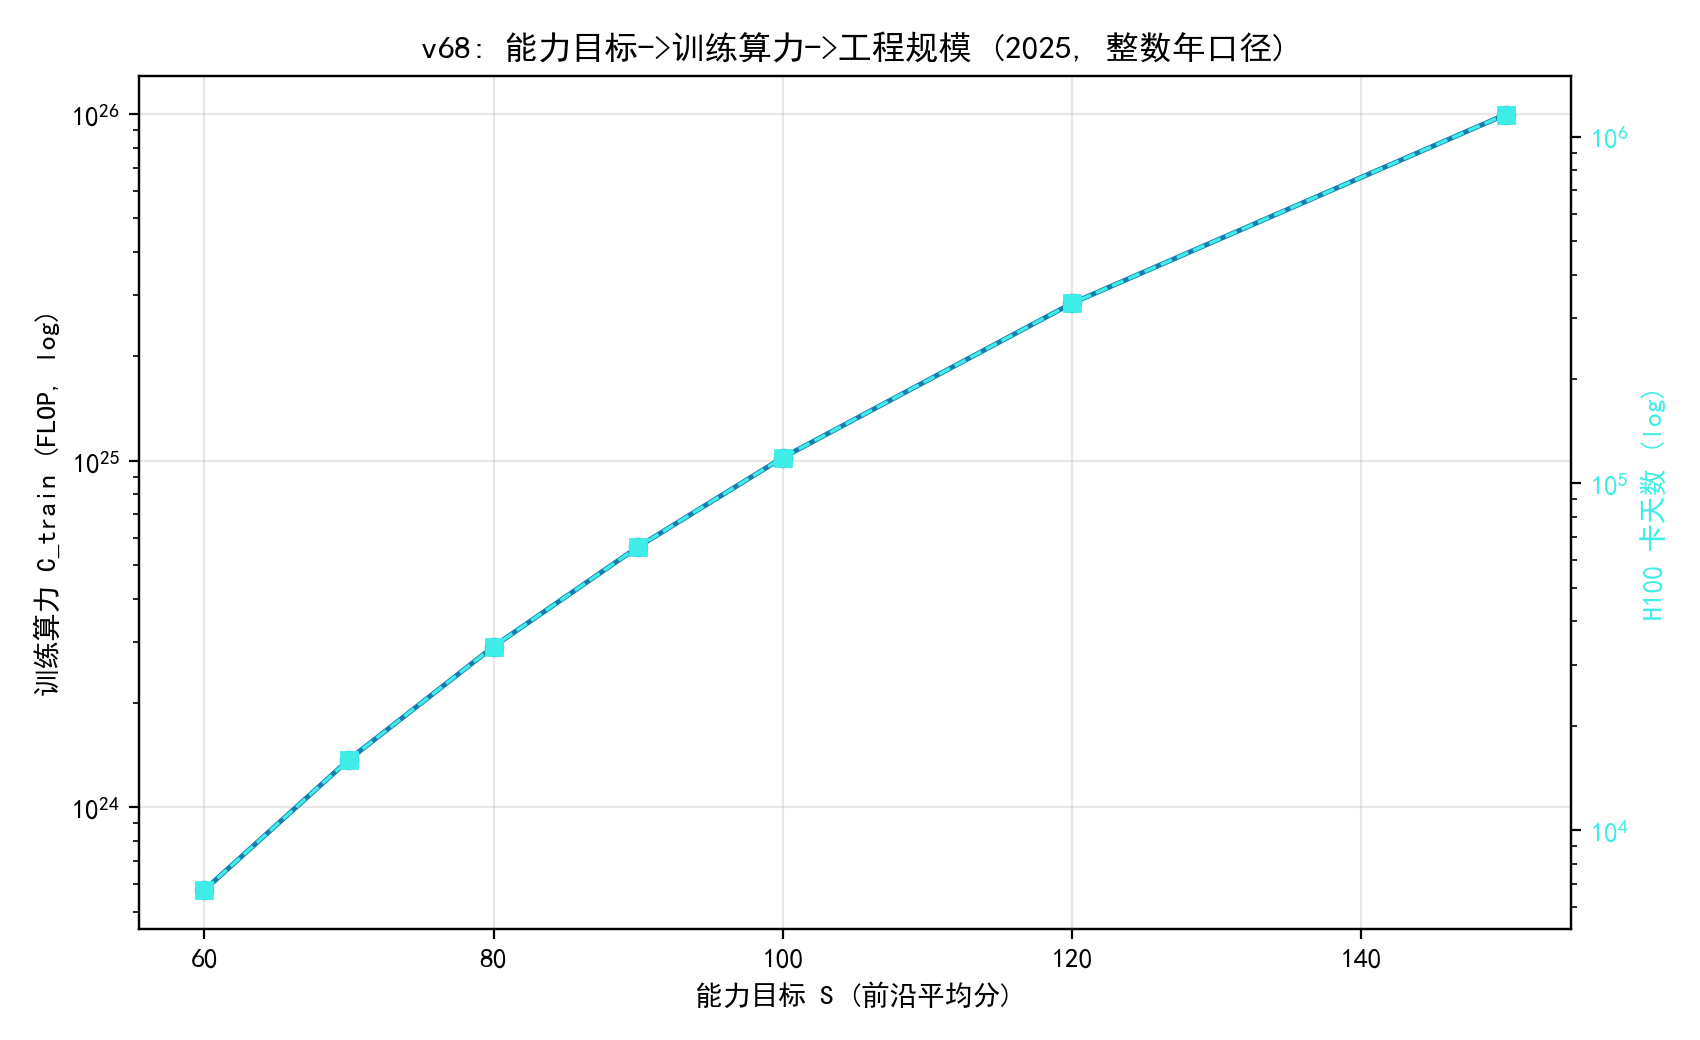
\includegraphics[width=0.82\textwidth]{figures/v68_p4_compute_conversion.png}
\caption{能力目标 $\to$ 训练算力（对数轴）：S=90 约需 6.6 万卡天。}
\label{fig:p4_computeconv}
\end{figure}

\textbf{规模--时间的等能力线}（图 \ref{fig:p4_isoquant}）：由 QR90 得
$\partial\ln N/\partial t=-b_T/b_N=-0.245$——在能力前沿上\textbf{时间与
规模可互换}：每多等 1 年，达到同一能力所需的参数量可减少约 \textbf{22\%}
（或提前 1 年需支付约 28\% 的参数溢价）。等能力线族（$S\in\{60,\dots,
100\}$）给出``算力约束下的时间折现''：算力受限者可通过\textbf{等待}
降低参数需求（$-22\%$/年），追赶进度者需\textbf{提前投入}换取规模溢价。
与算力落地换算（v68）配合，构成 ``能力目标 $\to$ 预算 $\times$ 时间'' 的
完整决策面。

\begin{figure}[htbp]
\centering
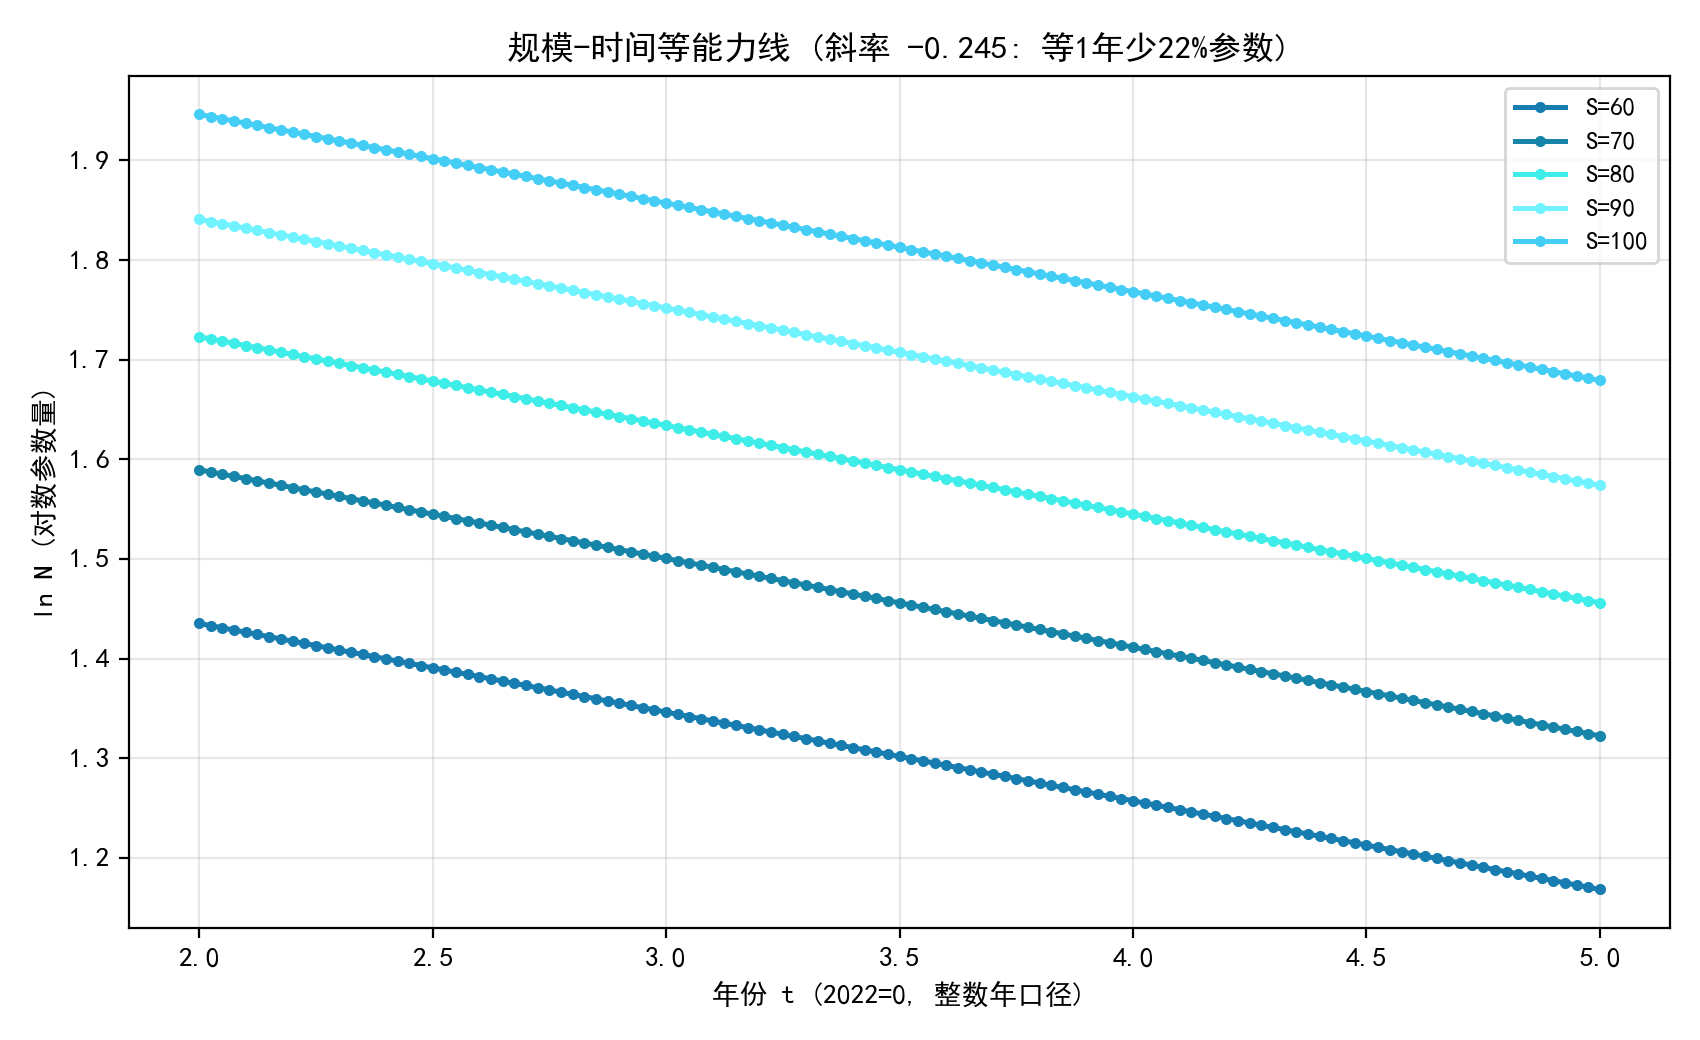
\includegraphics[width=0.8\textwidth]{figures/v71_p4_isoquant.png}
\caption{规模--时间等能力线：等 1 年少用 22\% 参数（斜率 −0.245）。}
\label{fig:p4_isoquant}
\end{figure}

\textbf{增速假设敏感性}（图 \ref{fig:p4_gNsens}）：预测的核心外生假设是
参数量年均对数增速 $g_N$（基准 1.251）。在
$g_N\in[0.4,1.6]$ 内扫描得到：12 个月前沿在 52.8--81.7 之间（相对基准
$\pm40\%$），24 个月在 66.8--160.0 之间（$\pm75\%$）——预测期越长，对
$g_N$ 的敏感度越高，且该敏感度远超分解口径（tau 0.8/0.9）与自助采样
带来的不确定性。这为``双情景 + 区间''的必要性提供了最直接的理由：
$g_N$ 假设本身的偏离是预测不确定性的最大来源。

\begin{figure}[htbp]
\centering
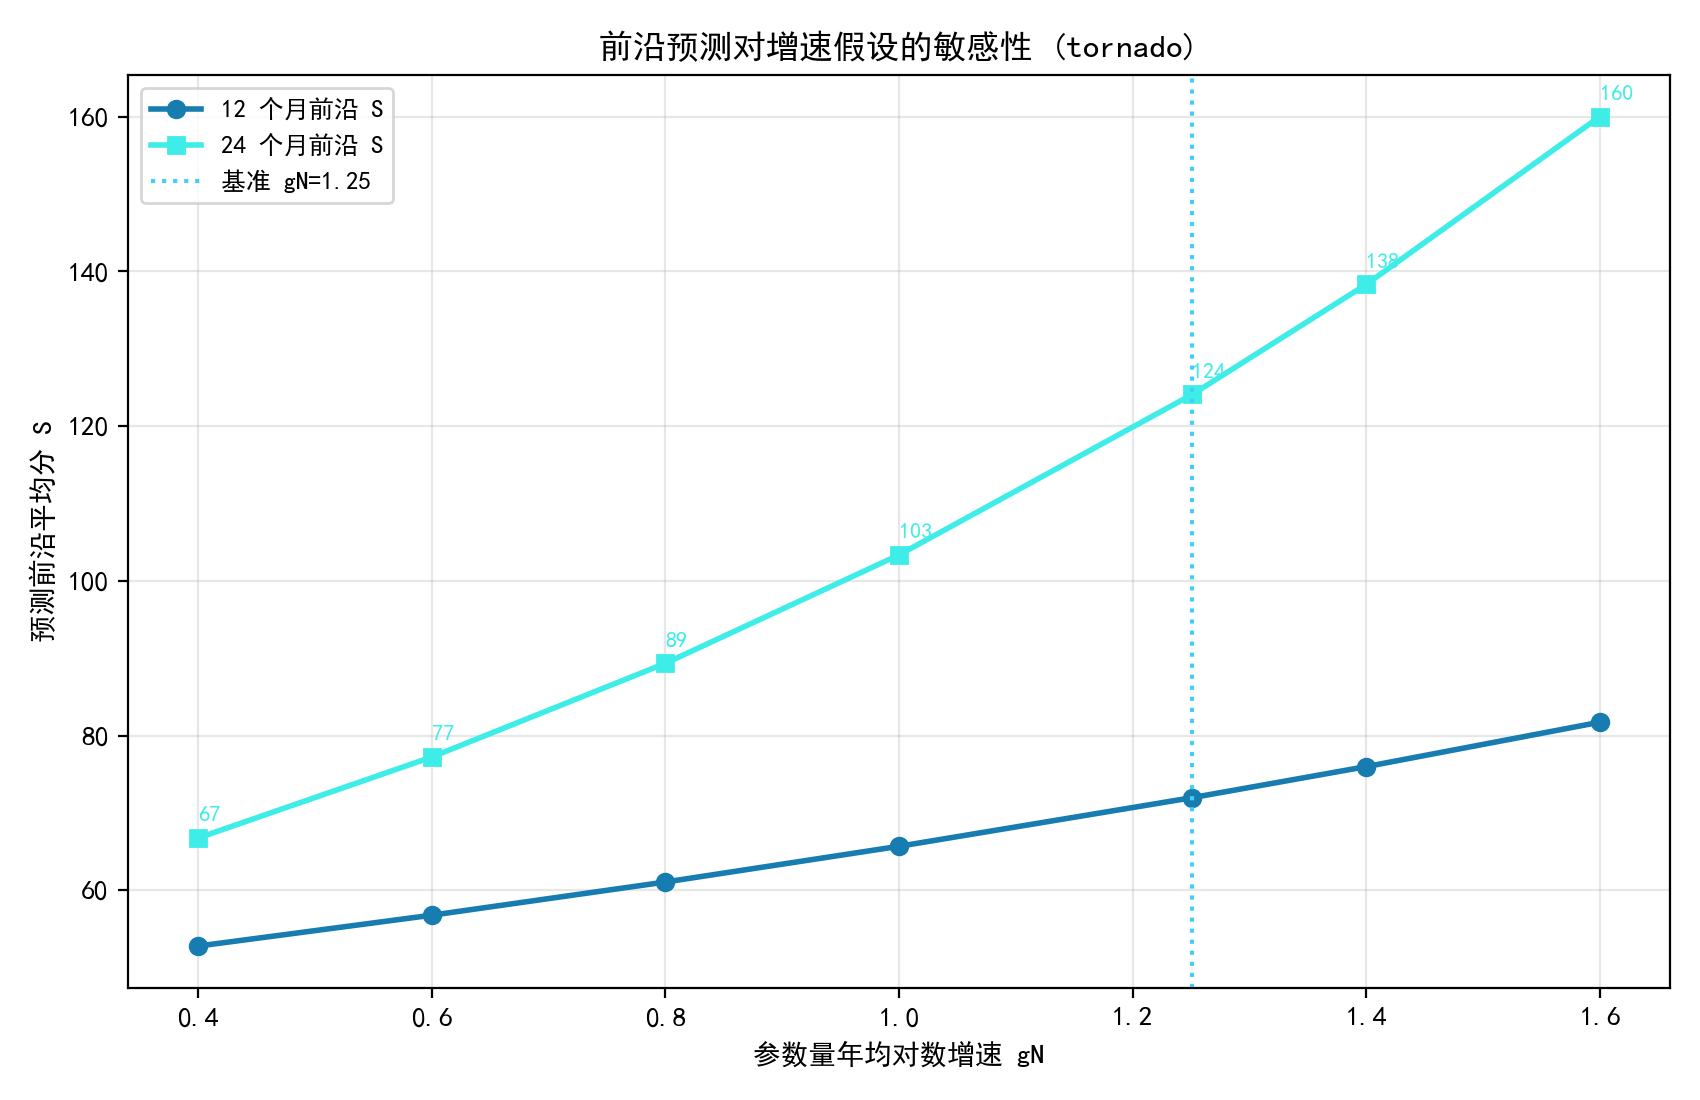
\includegraphics[width=0.82\textwidth]{figures/v34_p4_gN_sens.png}
\caption{前沿预测对参数量增速假设 $g_N$ 的敏感性（12/24 个月）。}
\label{fig:p4_gNsens}
\end{figure}

\textbf{历史回测（验证外推口径）}：用截至 $y_0$ 年的数据拟合分位数回归并
外推下一年/下两年的前沿，回测结果（表 \ref{tab:backtest}）显示：从 2023
或 2024 截断外推 2024/2025 前沿均系统性高估（+105\%$\sim$+276\%），因为
断点前的技术增速（滚动窗口首窗 $b_T$ 曾高达约 $1.1$/年）不能延续——
2024 下半年起前沿增速
结构性放缓（见灵敏度节 Chow 检验）。该回测直接支持正文做法：预测必须使用
包含断点后样本的全样本分位数回归（$b_T=0.089$），并对放缓情景单独建模。

\begin{table}[htbp]
\centering
\caption{前沿预测的历史回测：截至 $y_0$ 外推与 2024/2025 实际前沿对照}
\label{tab:backtest}
\begin{tabular}{c|c|c|c|c}
\toprule
$y_0$ & 预测目标 & 预测 $S$ & 实际（数据口径） & 误差 \\
\midrule
2023 & 2024 & 70.9 & 34.6 & $+105\%$ \\
2023 & 2025 & 152.0 & 40.4 & $+276\%$ \\
2024 & 2025 & 102.0 & 40.4 & $+152\%$ \\
\bottomrule
\end{tabular}
\end{table}

\textbf{趋势形式的回测对比（模型形式风险）}：在表 \ref{tab:backtest} 同一
窗口集上，对 0.9 分位数目标（pinball 损失，L-BFGS-B 最小化）比较四种趋势
形式——线性（主链路）、二次（含 $t^2$ 项）、饱和渐近
（$g(1-e^{-\lambda t})$）与零增长基线（前沿停于 $y_0$ 数据 90 分位）。
样本外 MAPE：线性 178\%、二次 71\%、饱和 57\%、零增长 10\%（v82）——
断点前的线性外推系统性高估（与表 \ref{tab:backtest} 一致），饱和/二次形式
误差降至约三分之一，短窗上零增长最低亦印证 2024 下半年起的前沿减速。
仍需强调：\textbf{全样本}（含断点后信息）拟合下，饱和与二次形式对
12/24 个月前沿的投影为 $64.1/102.7$，\textbf{恰好落在双情景区间}
$[57.1,\,71.7]$ 与 $[78.6,\,123.9]$ 之内——主链路的``基础 vs 放缓''双情景
区间已\textbf{覆盖备选趋势形式的模型风险}，预测结论对趋势形式选择稳健
（``前沿持续上升、规模贡献主导''不变；最保守的零增长参照为 2025 水平
$S=40.4$ 不再上行）。\textbf{集成口径进一步收窄形式风险}（v86）：以回测
MAPE 反比加权三种趋势形式（线性 178\%、二次 71\%、饱和 57\% 的倒数作权），
12/24 个月投影为 $65.2/105.9$；等权平均（$66.6/109.7$）与饱和单形式
（$64.1/102.7$）构成口径带 $[64.1,\,66.6]$ 与 $[102.7,\,109.7]$，全部落
在双情景区间内——预测结论对趋势形式选择与集成口径双重稳健。

\textbf{年度前沿增速（减速的逐年证据）}：合并历史前沿与排行榜开源行，
逐年前沿 $S$ 为 35.0（2022）$\to$ 35.0（2023）$\to$ 51.2（2024）$\to$
47.2（2025）。年度对数增速 $\Delta\ln S$：2024 年为 $+0.381$（$+46\%$），
2025 年转负（$-0.082$，$-7.8\%$）；即前沿增速在 2024--2025 出现
\textbf{增速反转}（2022--2024 平均 $b_T=0.191$/年 vs 2025 年 $-0.082$/年）。
需要说明：2025 年样本仅含前三季度（排行榜更新至 2025-03），年度最大值
口径对样本时长敏感，因此该表与放缓情景（$b_T$ 减半）互为印证而非绝对
倒退的断言——与 Chow 断点检验（2024.5）方向一致。

\textbf{能力构成的演化}（图 \ref{fig:p4_taskgrowth}）：按任务拆分前沿
（2024-06 至 2025-03 开放行月度最大值），年化对数增速排序为
\textbf{MATH +0.89}、MUSR +0.54、GPQA +0.45、BBH +0.32、MMLU-PRO +0.20、
\textbf{IFEval +0.03（近饱和）}——数学/科学推理类任务增长最快，指令跟随
与百科知识类接近饱和。前沿的能力构成正从``通用知识+指令跟随''向
``硬推理''迁移，说明非规模技术进步主要落在推理能力上（与时间通道
$b_T$ 的分解一致），也为``推理--成本权衡''场景提供了任务层面的微观依据。

\begin{figure}[htbp]
\centering
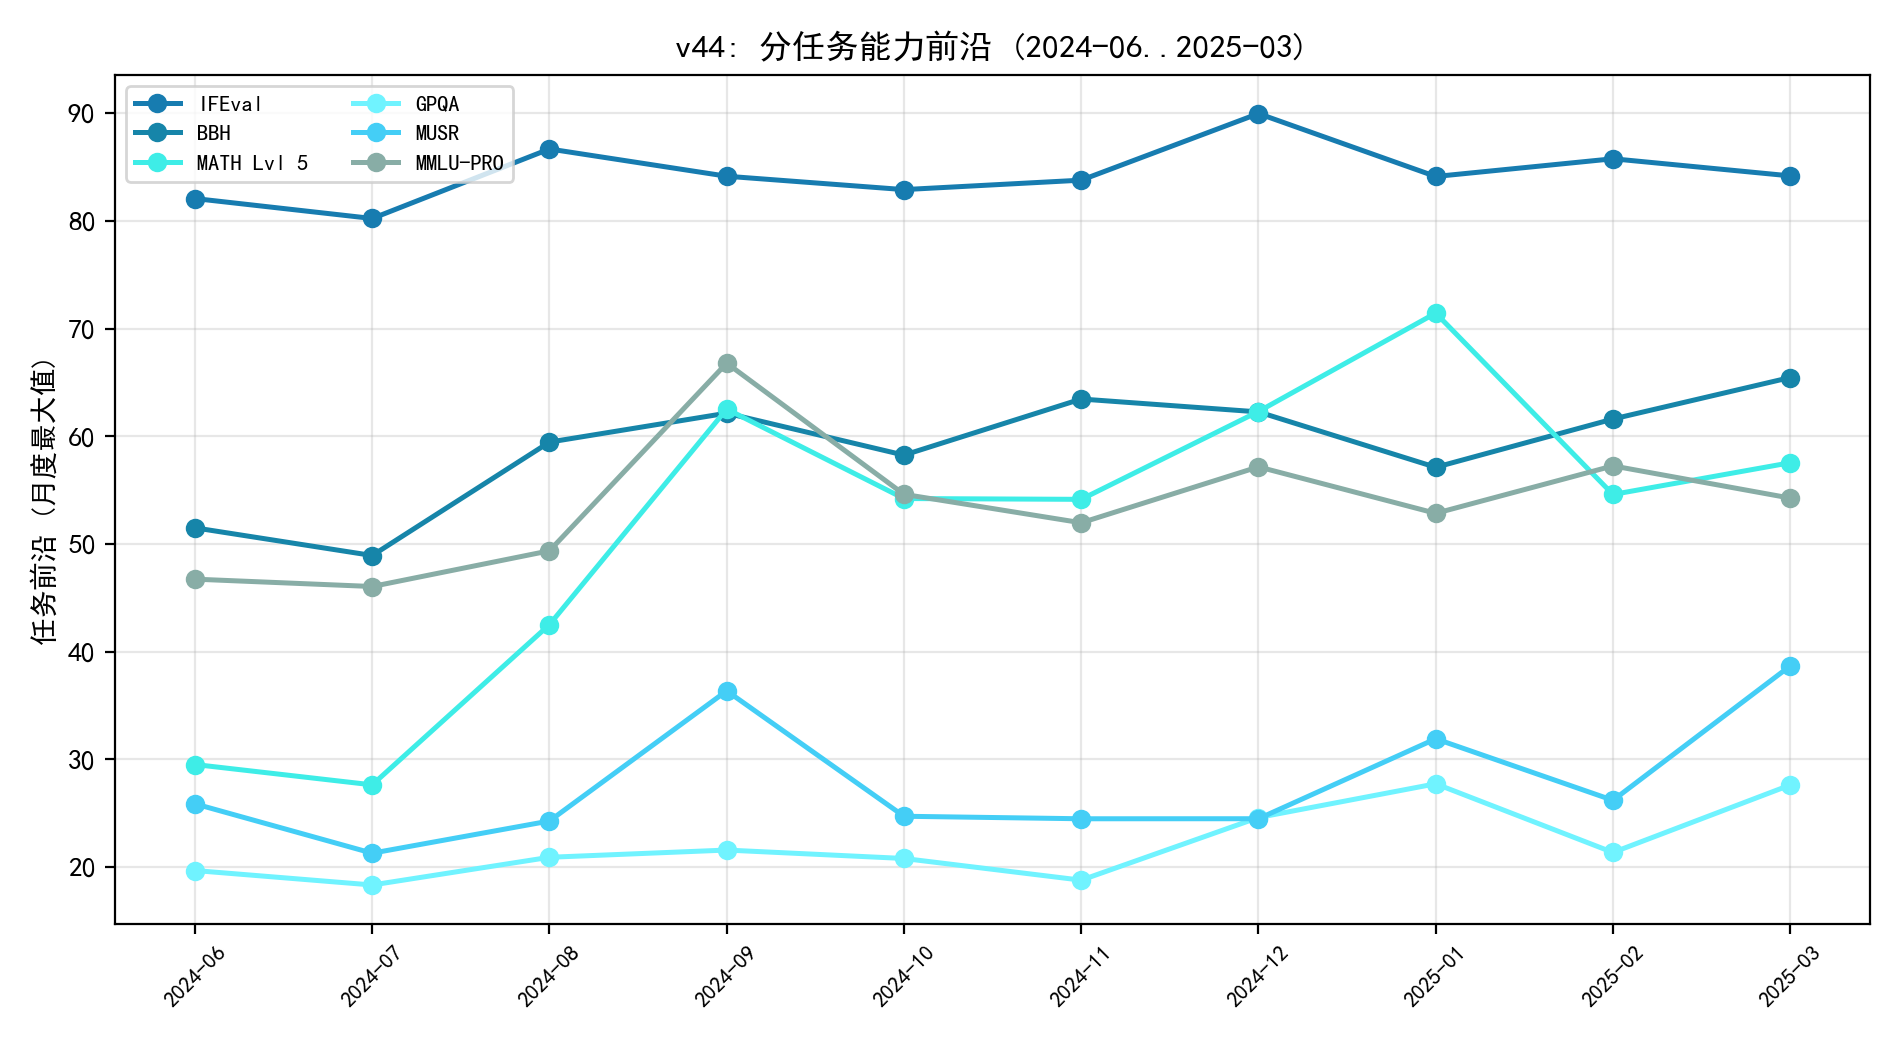
\includegraphics[width=0.86\textwidth]{figures/v44_p4_task_growth.png}
\caption{分任务能力前沿：推理类（MATH/GPQA/MUSR）增长快于知识/指令类。}
\label{fig:p4_taskgrowth}
\end{figure}

\textbf{规模分桶的增速梯度}（图 \ref{fig:p4_scalebucket}）：从任务维度转到
\textbf{规模维度}，把开放模型按参数分 5 桶，拟合各桶 90 分位分的年化
增速：$0.3$--$1$B +5.61、$1$--$3$B +3.56、$3$--$10$B +4.85、
\textbf{$10$--$30$B +9.46（最快）}、$30$--$100$B +3.09（最慢）。
梯度\textbf{非单调}：$10$--$30$B 的``甜点区''前沿进步最快（该规模段在
窗口内集中发布且质量快速爬升），$30$--$100$B 头部大模型基数高、边际
放缓最明显，小桶（$0.3$--$1$B）亦有较快进步（技术下放/蒸馏）。任务侧
（v44）与规模侧（本段）合起来构成前沿演进的\textbf{完整画像}：能力向
硬推理迁移 + 中大规模段进步最快。

\begin{figure}[htbp]
\centering
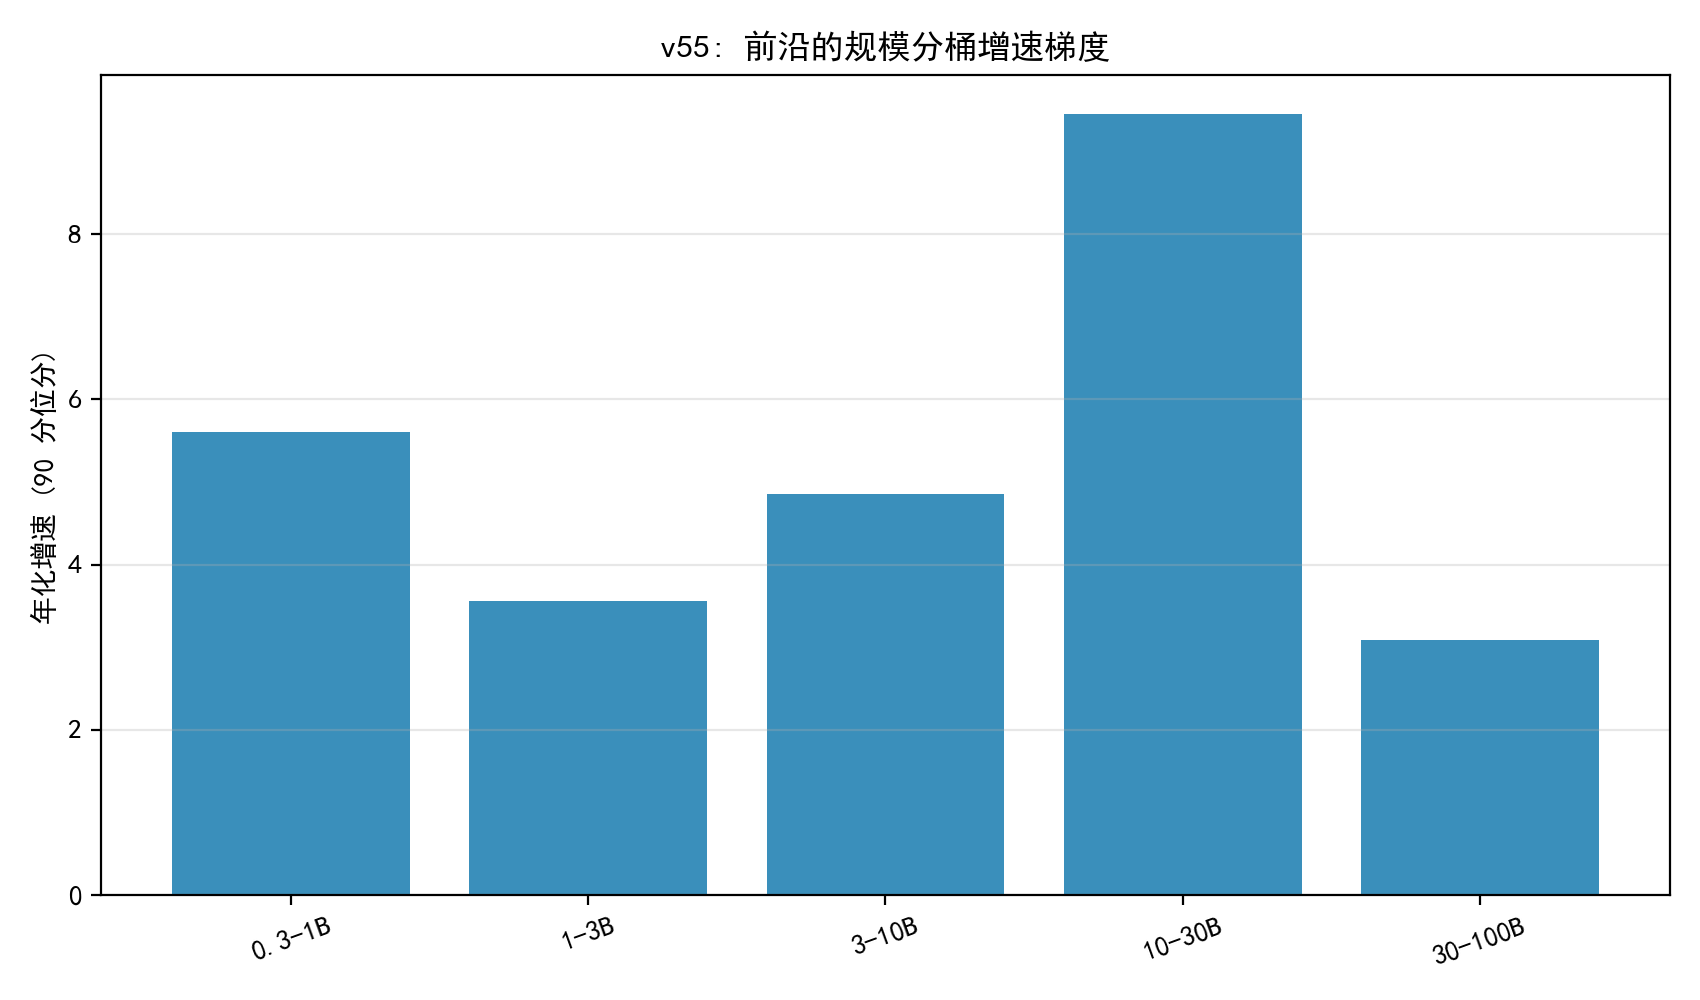
\includegraphics[width=0.8\textwidth]{figures/v55_p4_scale_bucket.png}
\caption{规模分桶的前沿年化增速：10--30B 甜点区最快，30--100B 最慢。}
\label{fig:p4_scalebucket}
\end{figure}

\textbf{任务 $\times$ 规模二维增速}（图 \ref{fig:p4_taskscale}）：把任务
维度（v44）与规模维度（v55）合成热图（各桶 90 分位年化增速）：MATH
全域最快且在 $1$--$3$B（+2.52）与 $10$--$30$B（+2.45）\textbf{双峰}；
GPQA 峰值在 $10$--$30$B（+1.27）但 $3$--$10$B 近零（+0.02）；
$10$--$30$B 在 6 个任务中 5 个增速领先或次高（呼应 v55 甜点区）；
$30$--$100$B 普遍放缓（除 MATH +1.13）；$0.3$--$1$B 推理类快速
（MATH +1.26/GPQA +0.56）但 MUSR $-0.72$ 下滑；IFEval 在 $1$--$3$B
+0.93、大桶饱和（$-0.03$）。\textbf{推理增速的规模分布呈双峰}（技术
下放 + 中大规模优化），任务侧与规模侧交叉验证，构成能力 $\times$ 规模的
完整二维画像。

\begin{figure}[htbp]
\centering
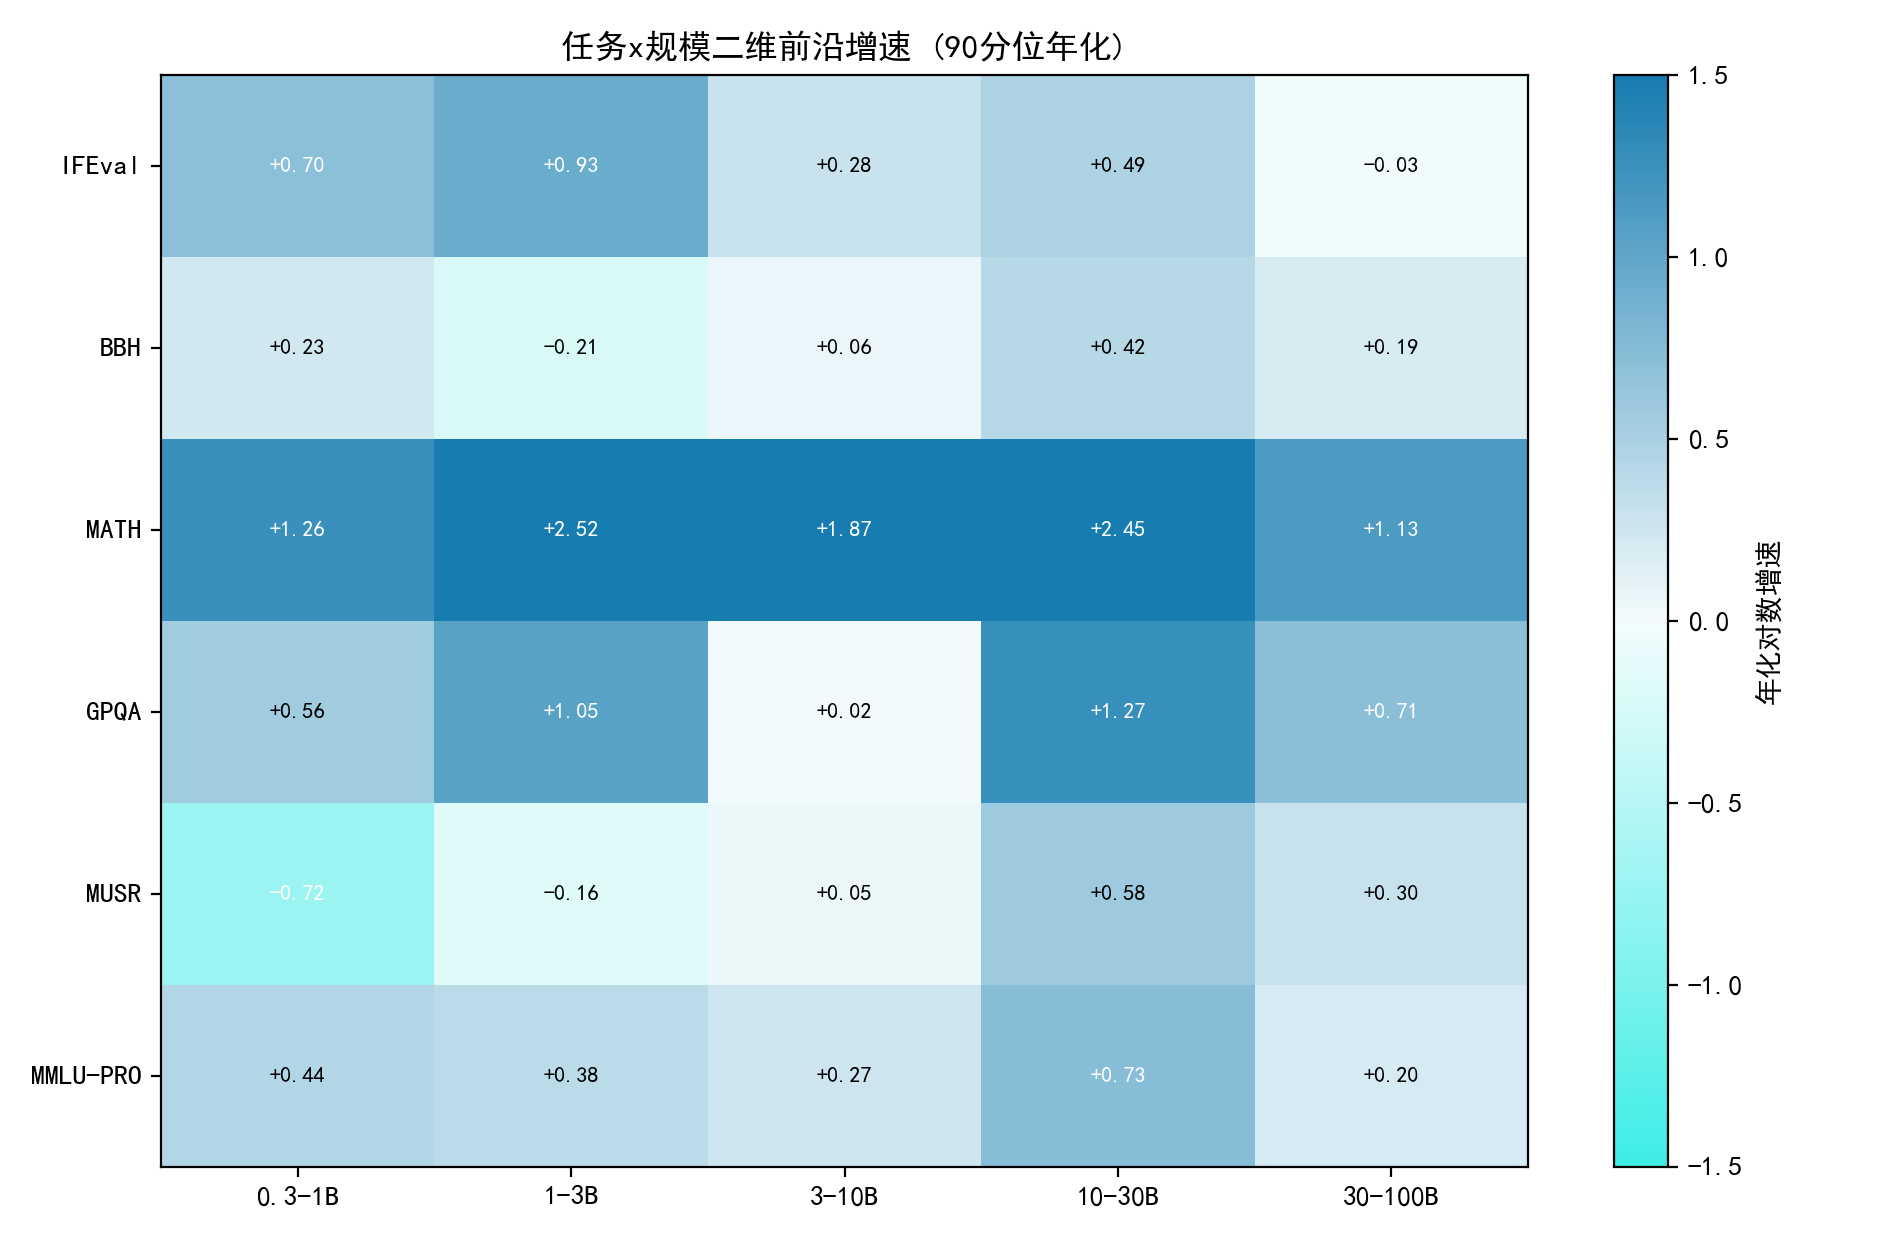
\includegraphics[width=0.85\textwidth]{figures/v63_p4_task_scale.png}
\caption{任务 $\times$ 规模二维前沿增速：MATH/GPQA 在 1--3B 与 10--30B 双峰。}
\label{fig:p4_taskscale}
\end{figure}

\textbf{分层演进：分化还是普惠}（图 \ref{fig:p4_stratify}）：按分位层
（p50/p75/p90）比较年化增速。\textbf{全域}：p50 +0.30、p75 +0.69、
p90 +0.62，p90/p50 比 \textbf{2.04}——顶层增速约为中位的两倍，
\textbf{顶层分化}（能力进步集中在头部）。但按规模段看，\textbf{段内是
普惠式提升}：$1$--$3$B 段 p50 +0.59 快于 p90 +0.30（比 0.50），
$10$--$30$B 段 p50 +1.04 也快于 p90 +0.79（比 0.76）。综合含义：
全域分化主要来自\textbf{规模段间差距扩大}（中段整体被抬升 + 头部大模型
独享），段内各层同步进步——与 v59 两端滞后、v55 甜点区相互印证，
``普惠与分化并存''。

\begin{figure}[htbp]
\centering
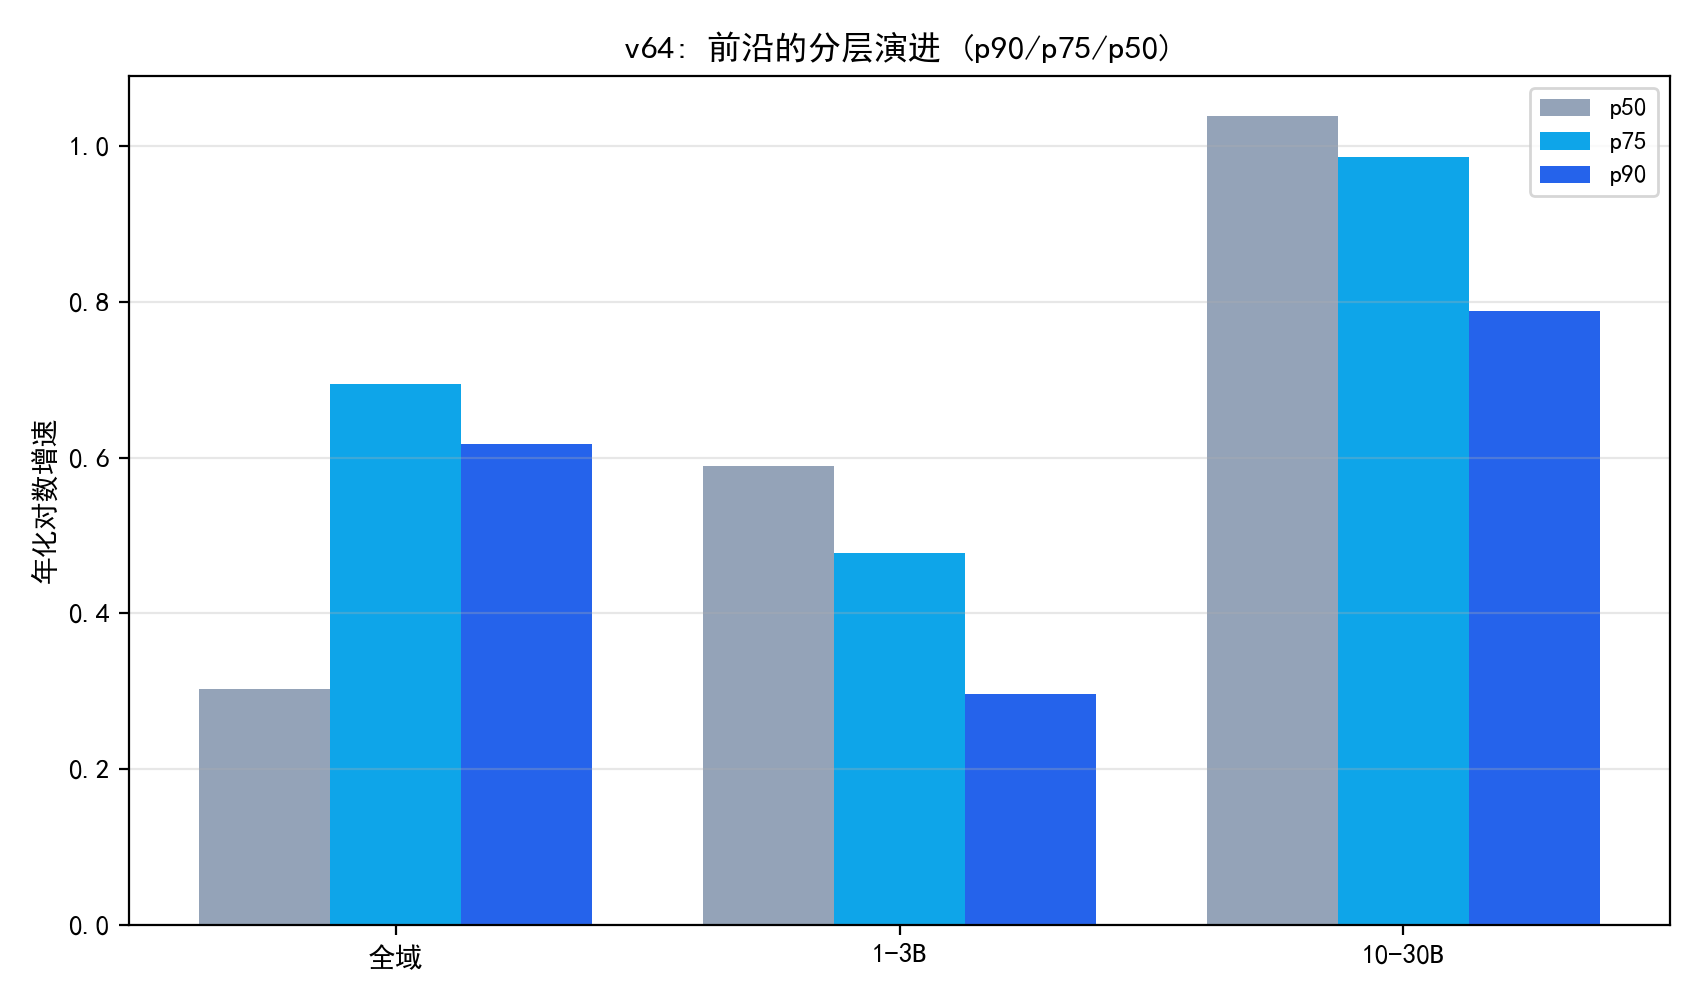
\includegraphics[width=0.8\textwidth]{figures/v64_p4_stratify.png}
\caption{分层演进：全域顶层分化（p90/p50≈2），段内普惠（p50 快于 p90）。}
\label{fig:p4_stratify}
\end{figure}

\textbf{滚动窗口参数核验}（图 \ref{fig:p4_rolling}）：以月度精度时间轴
$t$ 对四个截止窗口（2024-06 至 2025-03）滚动拟合 QR90。规模弹性 $b_N$
随窗口单调上升（$0.224\to0.338$，逼近全样本 $0.364$），而时间斜率 $b_T$
持续下降（$1.10\to0.50$/年）——2024 上半年开源模型的快速追赶（时间驱动）
在后续窗口显著减弱，规模驱动相对增强。滚动证据与年度前沿增速的
``增速反转''及 Chow 断点方向一致，进一步说明：\textbf{放缓主要来自时间
维度的外生驱动衰减，而非规模弹性的内生化衰退}。（注：本处采用月度精度
$t$，系数绝对水平与主链路年度粒度不同，但漂移趋势一致。）

\begin{figure}[htbp]
\centering
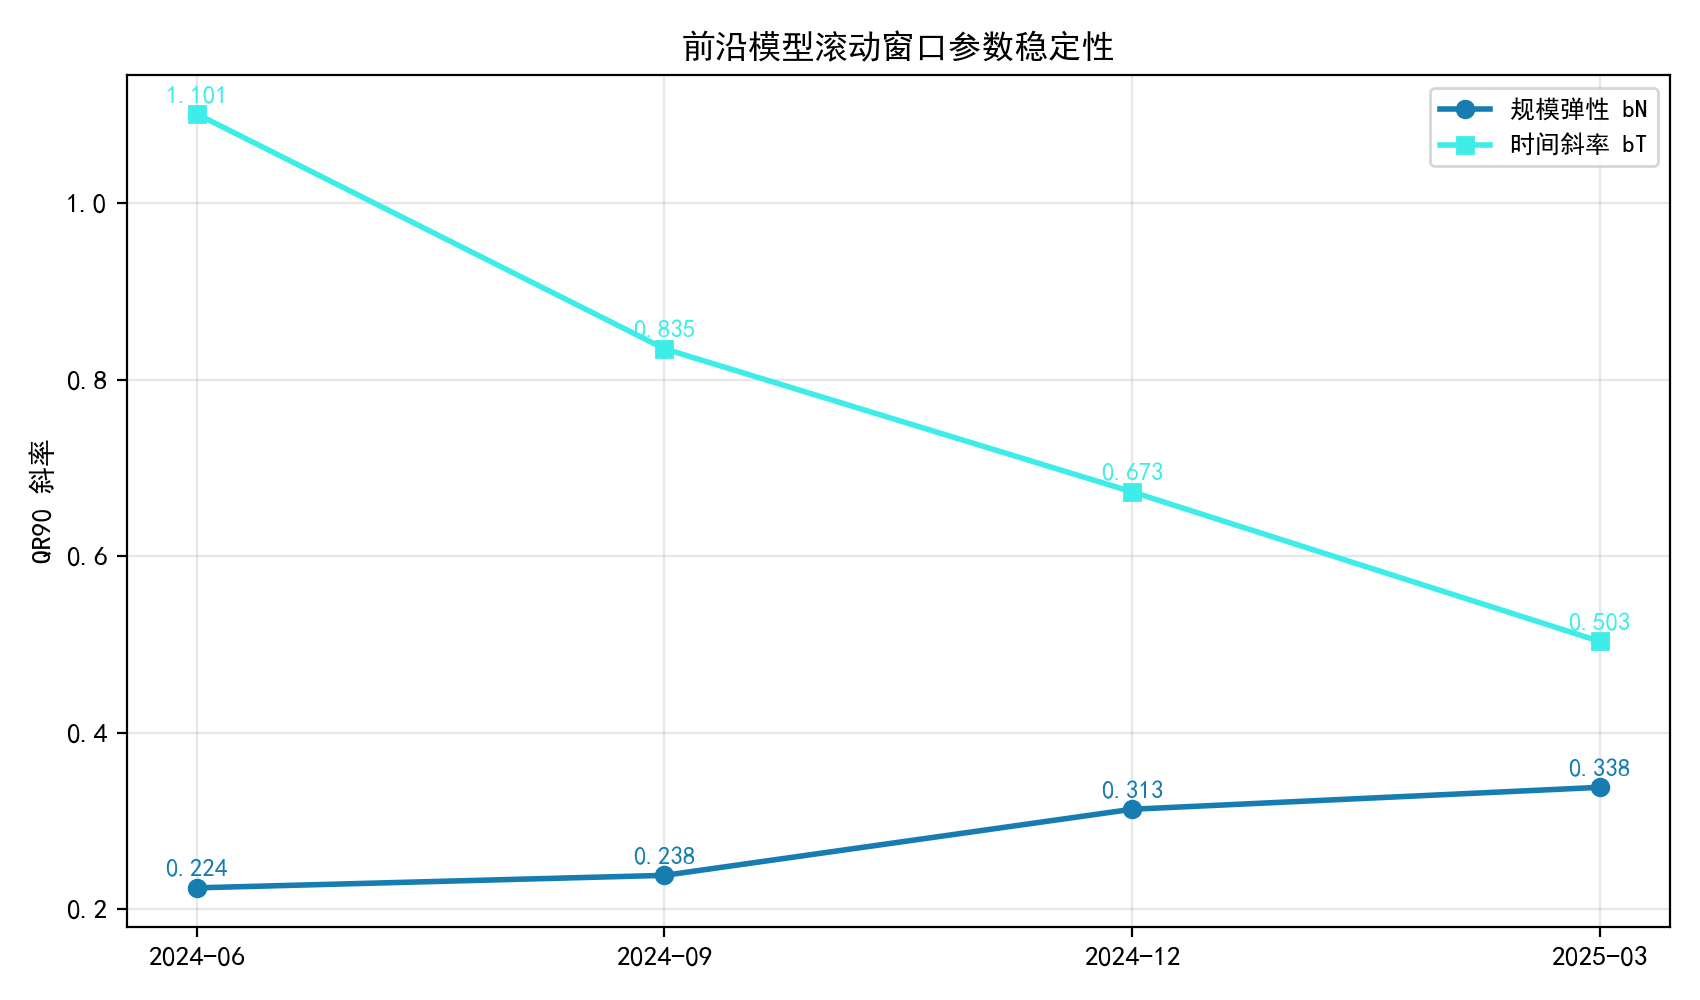
\includegraphics[width=0.82\textwidth]{figures/v32_p4_rolling.png}
\caption{前沿 QR90 滚动窗口参数：规模弹性上升、时间斜率持续下降。}
\label{fig:p4_rolling}
\end{figure}

\begin{figure}[htbp]
\centering
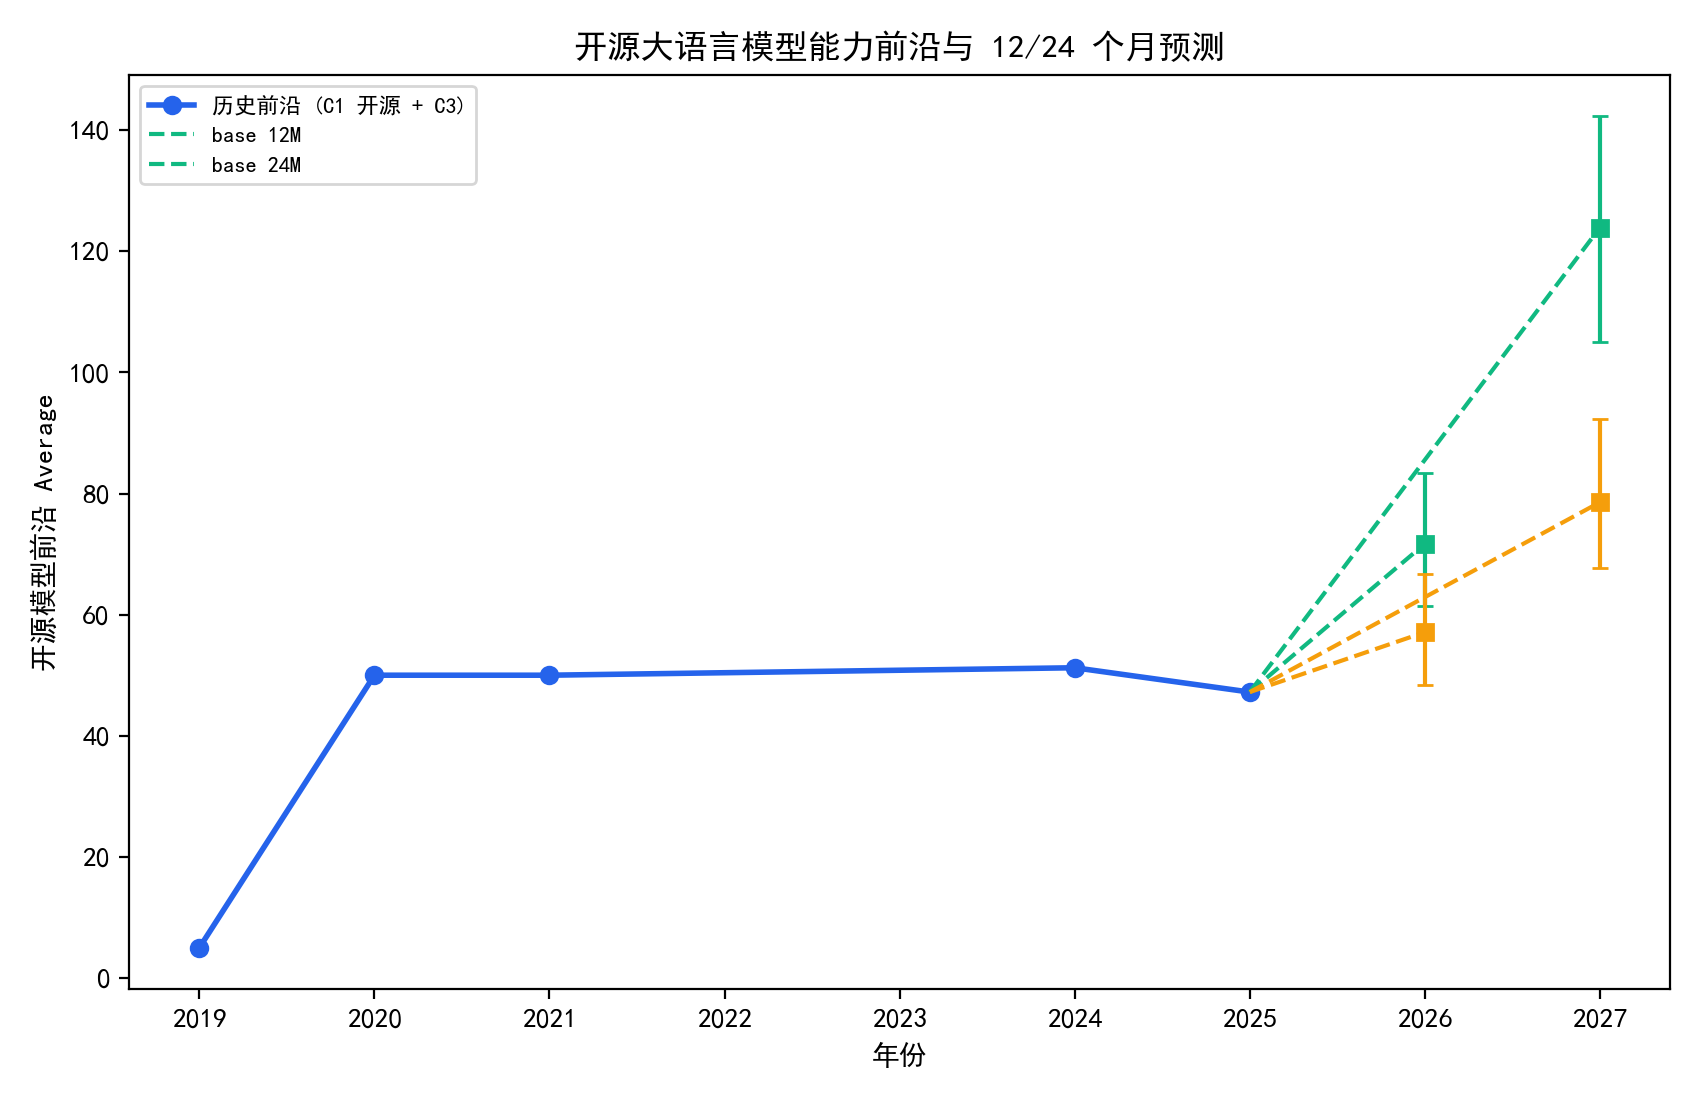
\includegraphics[width=0.88\textwidth]{figures/p4_frontier.png}
\caption{开源模型能力前沿（历史点）与 12/24 个月预测（基础/放缓情景，90\% 区间）。}
\label{fig:p4_frontier}
\end{figure}

前沿的\textbf{双驱动表面}（规模 $\ln N$ 与时间 $t$）以 3D 视图呈现于
图 \ref{fig:p4_3d}：0.9 分位数平面沿 $\ln N$ 轴斜率 $b_N=0.364$、沿时间轴
斜率 $b_T=0.089$，二者合成能力前沿——平面上 2025 前沿点（星标）与
2026/2027 预测点（三角）直接展示``规模外推 + 时间演进''的联合驱动机制。

\begin{figure}[htbp]
\centering
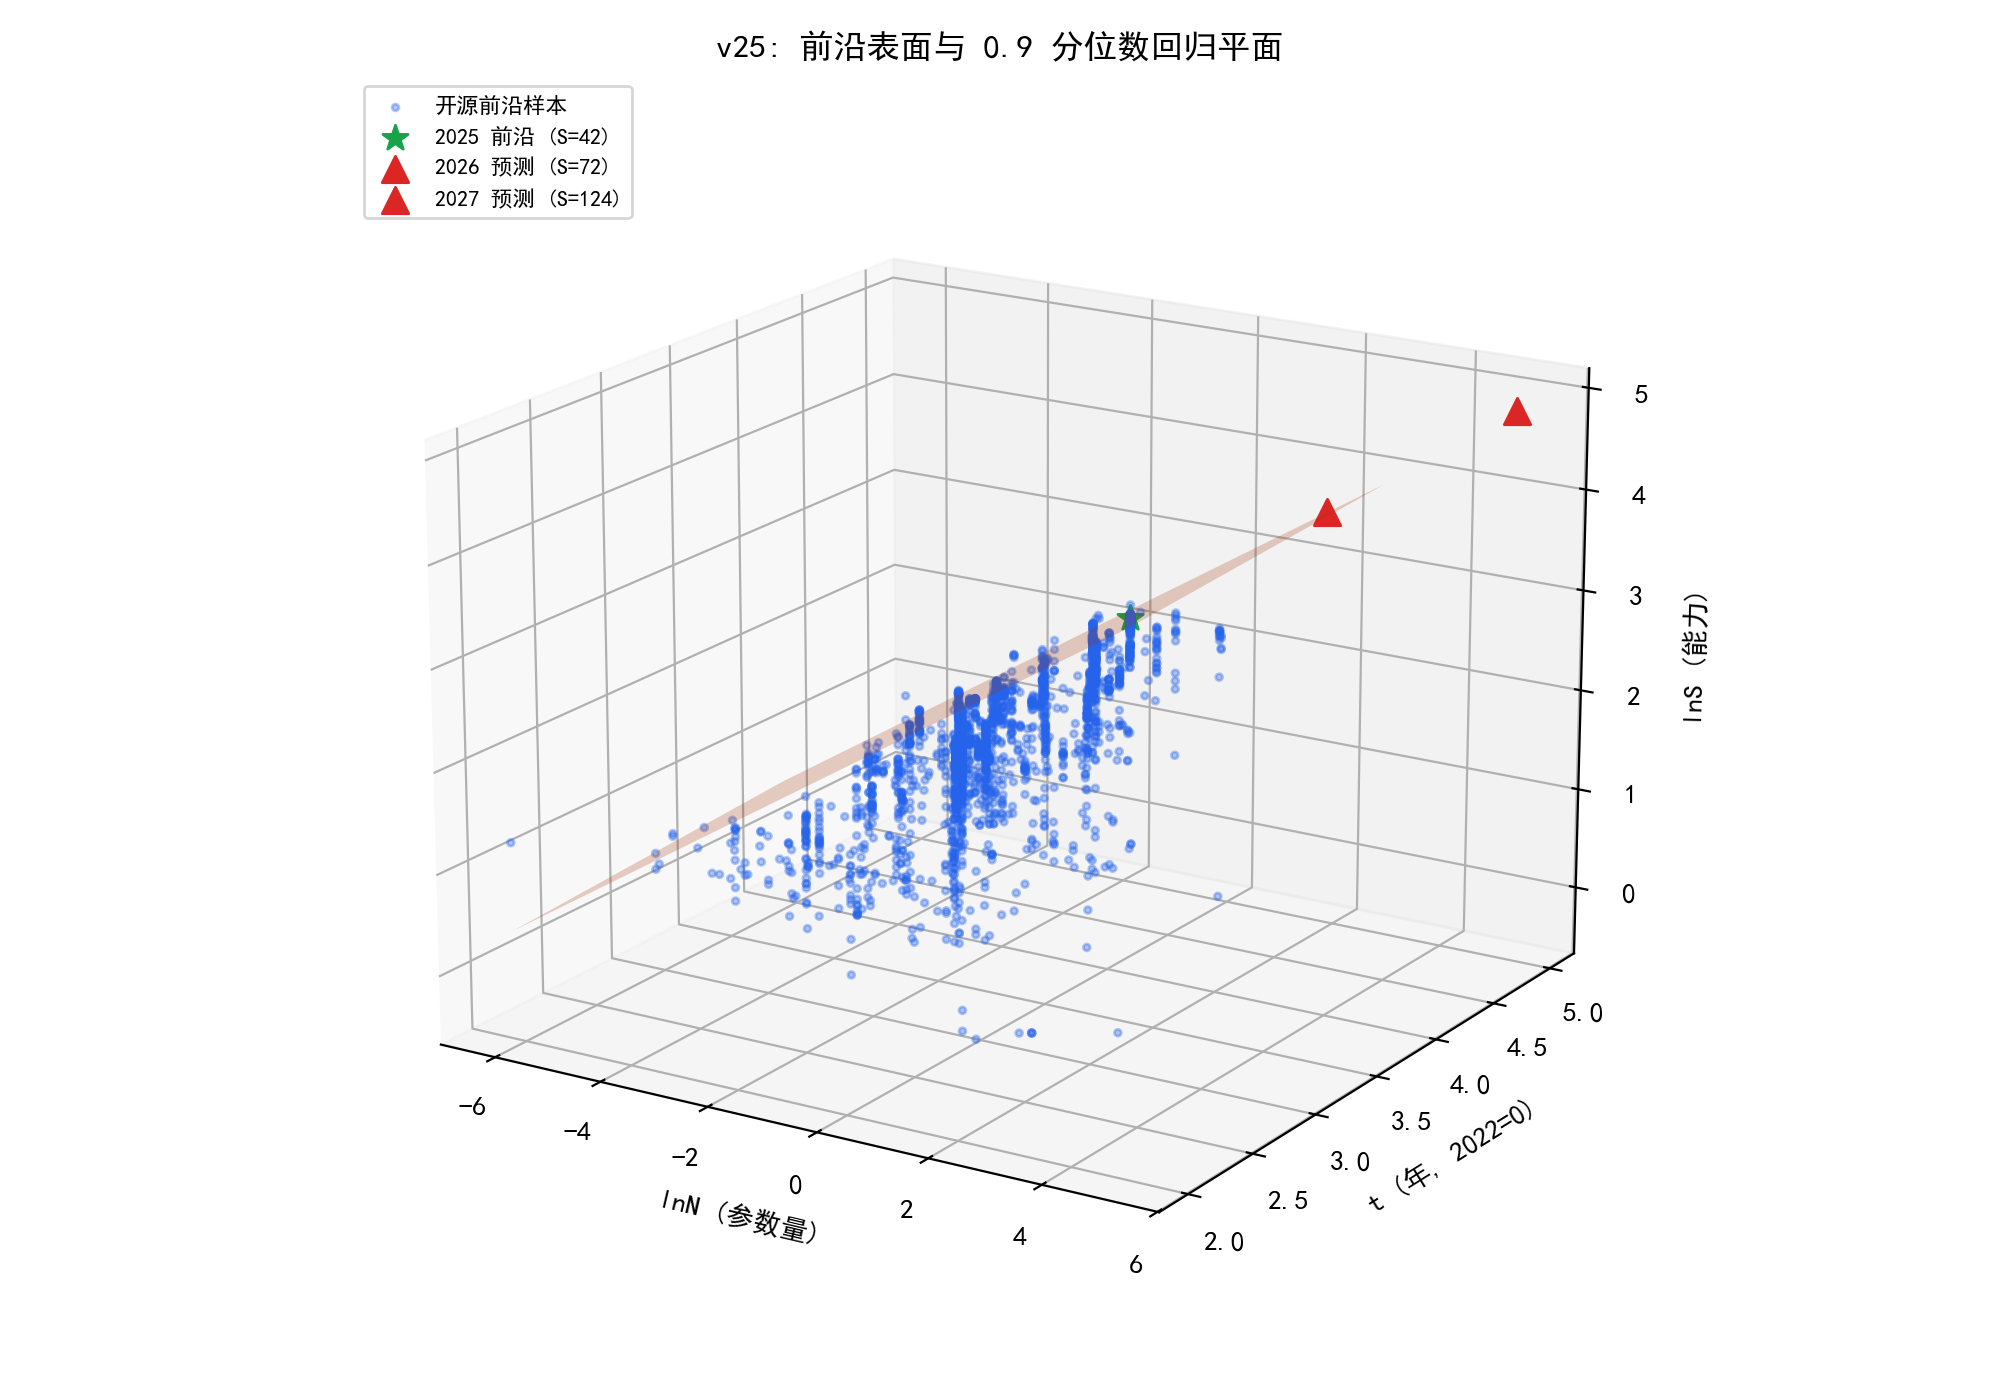
\includegraphics[width=0.88\textwidth]{figures/v25_p4_3d_surface.png}
\caption{能力前沿 3D 表面与 0.9 分位数回归平面（星标=2025 前沿，三角=预测点）。}
\label{fig:p4_3d}
\end{figure}

\textbf{家族留出验证}（图 \ref{fig:p4_familycv}）：把前沿模型按家族分桶
（llama/qwen/gemma/mistral/phi/yi/other 七族；样本 $n=2493$，其中
2484 条归族），逐个
家族留出拟合 $\ln S=c_0+b_N\ln N+b_T t$。全量 OLS 得 $b_N=0.366$
（与 QR90 的 0.364 一致，估计器稳健）；家族留出下 $b_N\in[0.353,0.384]$，
最大偏离约 5\%——\textbf{规模弹性跨家族稳定}，前沿斜率不是由单一家族
驱动。留出残差显示：qwen（+0.223）与 phi（+0.161）显著高于
规模--时间预测线（技术进步更快），llama/mistral 略低于线；留出 $R^2$
中 qwen 最高（0.588），gemma（0.109）与 phi（0.286）最低，说明这两家
族的分数更受个体因素影响。该验证同时说明：`双驱动''模型对领先家族的
``超出规模''能力（如 qwen）存在系统性低估，预测区间已涵盖此差异。

\begin{figure}[htbp]
\centering
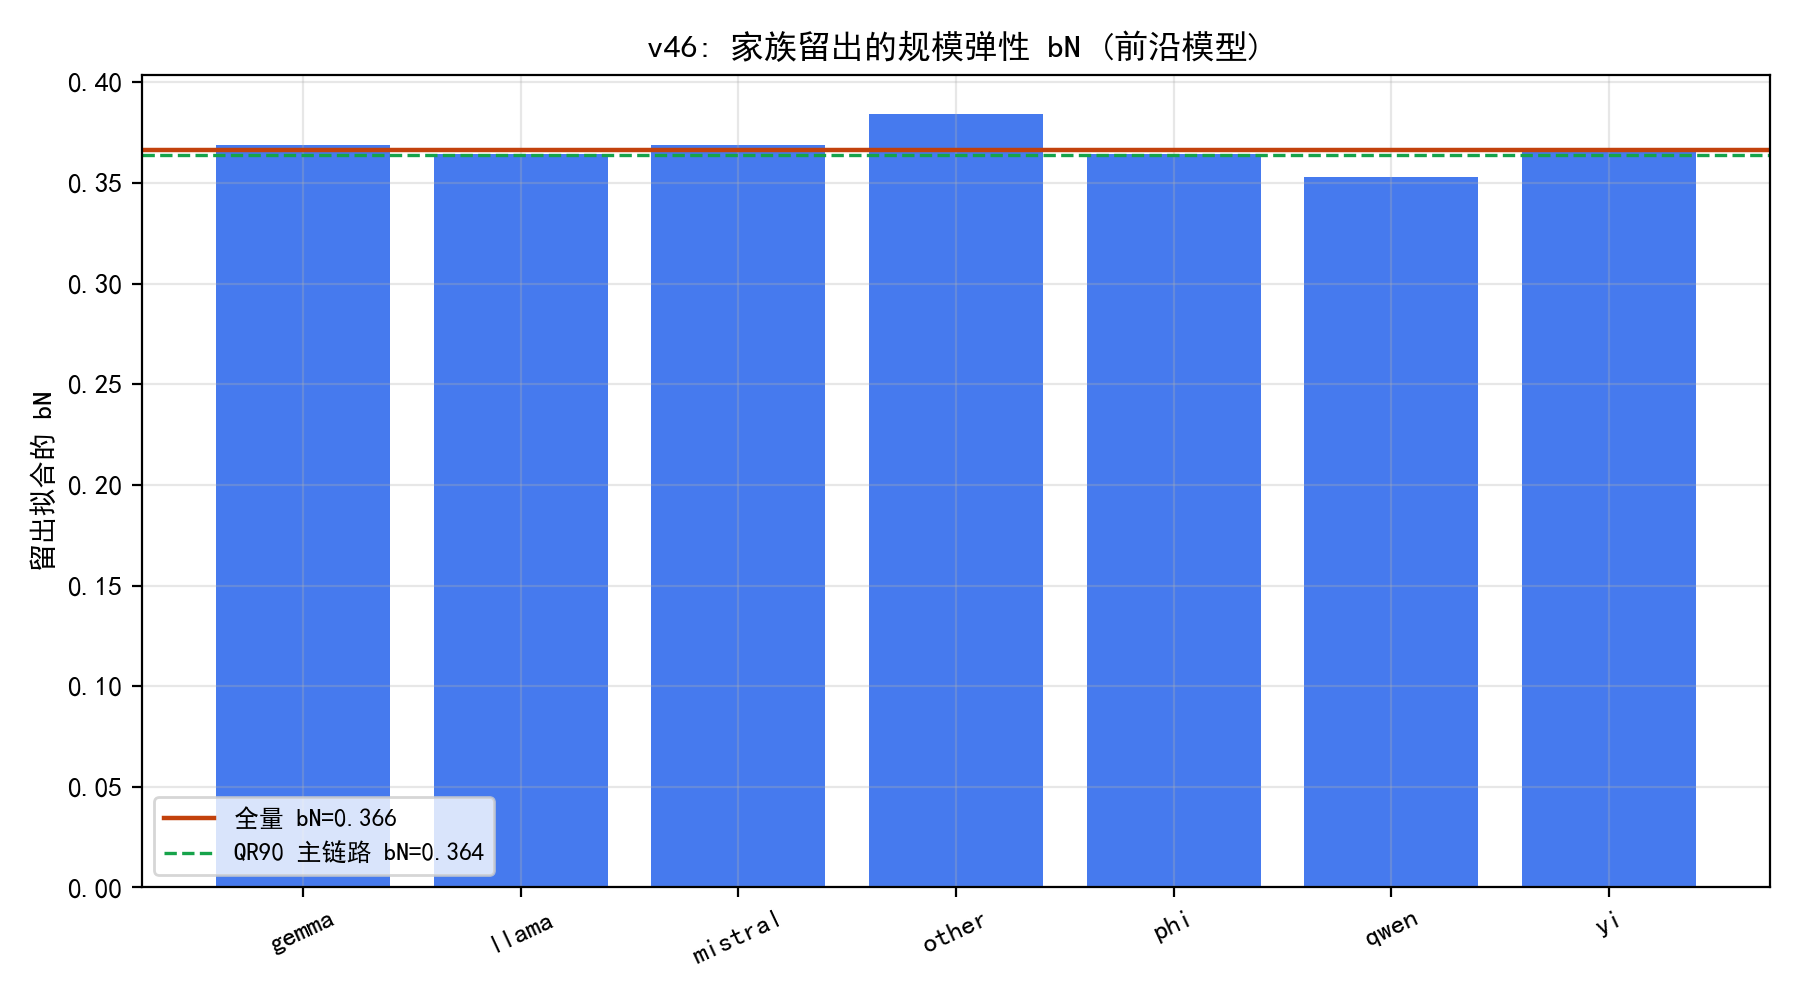
\includegraphics[width=0.8\textwidth]{figures/v46_p4_family_cv.png}
\caption{家族留出的规模弹性 $b_N$：全家族稳定在 0.36 附近。}
\label{fig:p4_familycv}
\end{figure}

\begin{figure}[htbp]
\centering
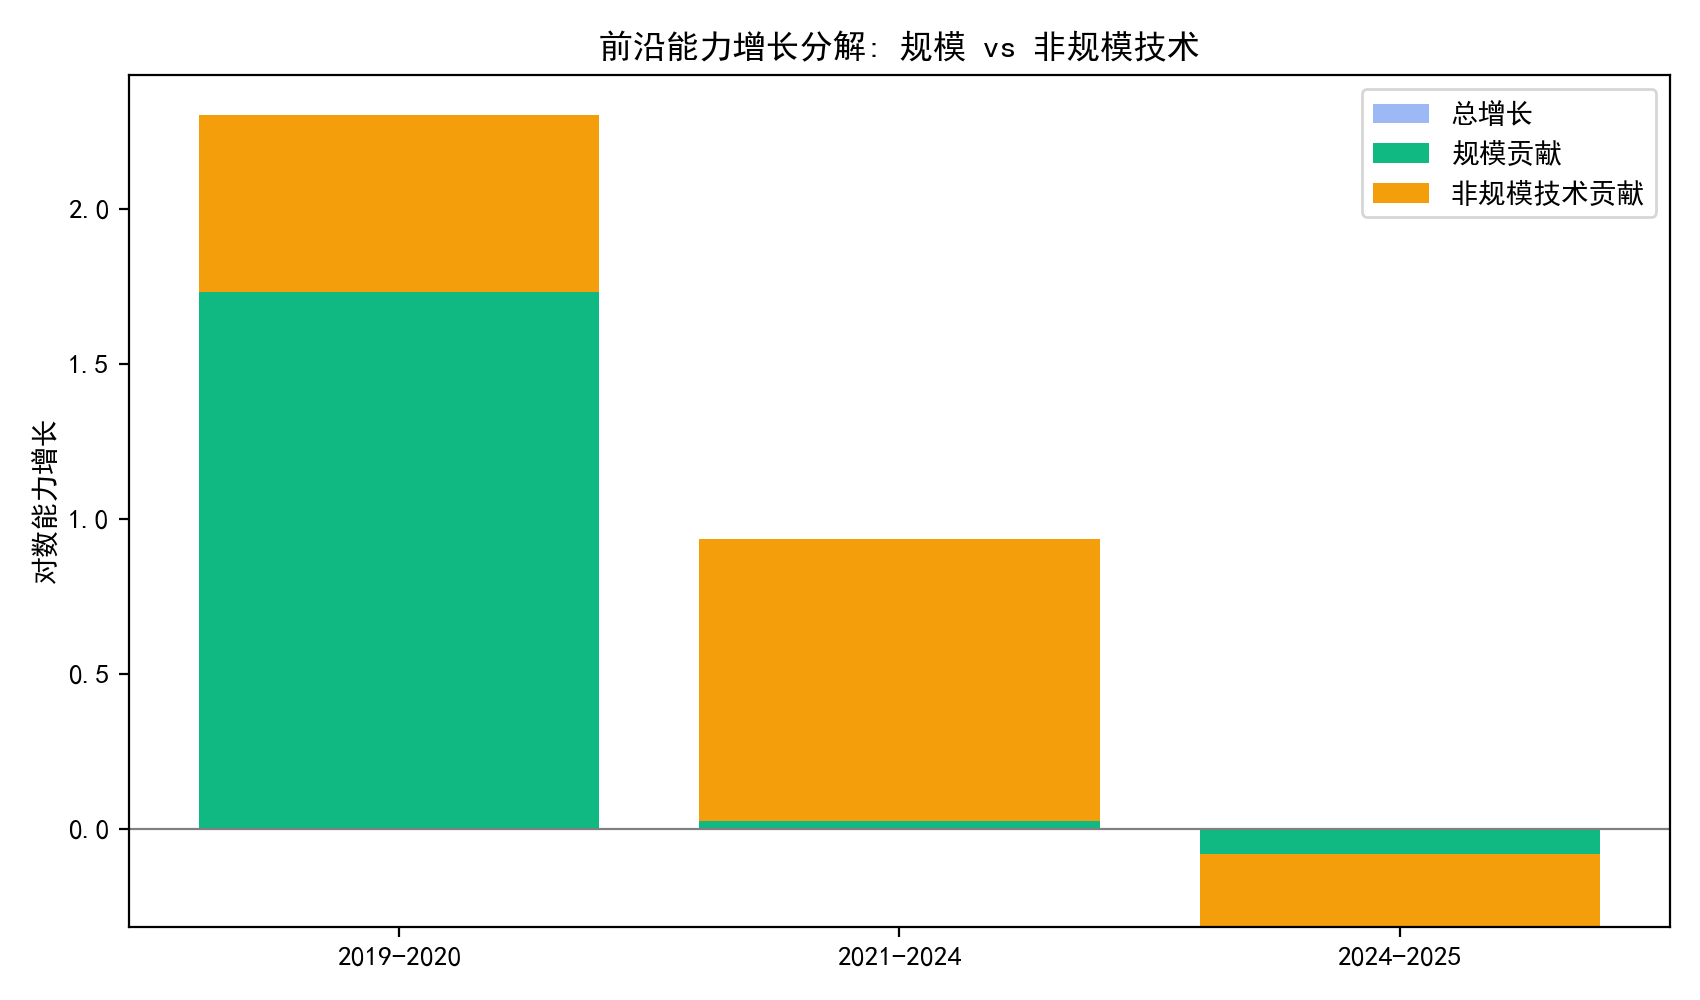
\includegraphics[width=0.8\textwidth]{figures/p4_decomposition.png}
\caption{前沿能力增长分解：规模贡献与非规模技术贡献。}
\label{fig:p4_decomp}
\end{figure}

\subsection{模型验证}

\paragraph{Loss--Benchmark 桥接（C6）}

为统一``损失''与``排行榜分''两套度量，用 C6 的 75 个模型的验证损失与
Benchmark 平均分建立 logit--log 线性映射：
\begin{equation}
\text{logit}\bigl(\tfrac{S}{100}\bigr)=0.852-3.304\ln L,
\qquad R^2=0.276\ (n=75).
\label{eq:bridge}
\end{equation}
映射误差按可比性分组：同一模型同一验证集（High）误差均值 $7.96\pm2.62$
分，不同验证集近似（Medium）为 $-3.13\pm10.26$ 分——说明桥接在中低精度
场景可用，且高可比性样本误差更集中。该桥接可将问题二的损失预测换算为能力
分，实现``资源 $\to$ 损失 $\to$ 能力''的完整链。

\begin{figure}[htbp]
\centering
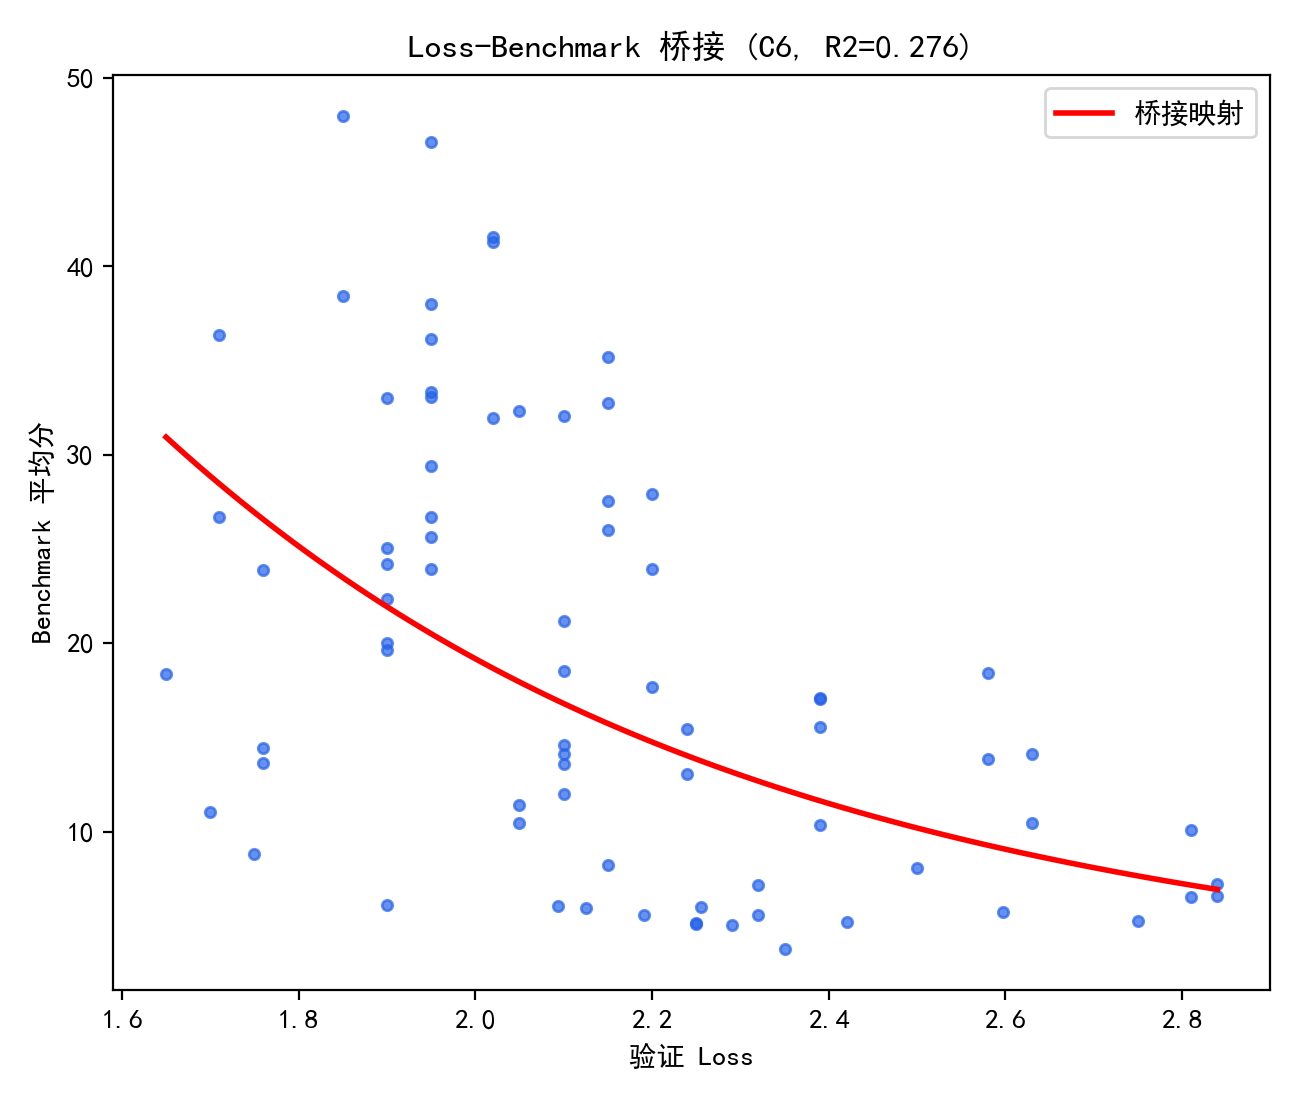
\includegraphics[width=0.62\textwidth]{figures/p4_bridge.png}
\caption{Loss--Benchmark 桥接映射（C6，75 个模型）。}
\label{fig:p4_bridge}
\end{figure}

\paragraph{C8 逐任务聚合分析}

从 C8 的 1863 个模型目录解析全部 JSON（跳过 4 个损坏文件，取每目录最新
记录，得 1860 个模型），提取 6 维逐任务 \texttt{acc}（IFEval 取
\texttt{inst\_level\_strict\_acc}、MATH 取 \texttt{exact\_match}、其余取
\texttt{acc\_norm}），聚合为模型级平均分：

\begin{table}[htbp]
\centering
\caption{C8 逐任务聚合得分（1860 模型）}
\begin{tabular}{c|cccccc}
\toprule
任务 & BBH & IFEval & MUSR & MMLU & GPQA & MATH \\
\midrule
平均 & 0.475 & 0.402 & 0.400 & 0.320 & 0.298 & 0.113 \\
标准差 & 0.116 & 0.215 & 0.046 & 0.130 & 0.039 & 0.120 \\
\bottomrule
\end{tabular}
\end{table}

任务难度排序（MATH 最难、BBH 相对最容易）与常识一致。将 C8 聚合分与 C1
排行榜平均分按模型名归一化匹配（$n=1895$），Spearman 相关 $=0.989$，说明
C8 逐任务明细与 C1 汇总高度一致，聚合口径可靠，可作为排行榜得分的独立
复算验证。同时 BBH/GPQA 等推理任务的内部子任务（如 BBH 的 27 个子任务）
也可逐项提取，用于刻画``推理能力谱''，此处从略。

\begin{figure}[htbp]
\centering
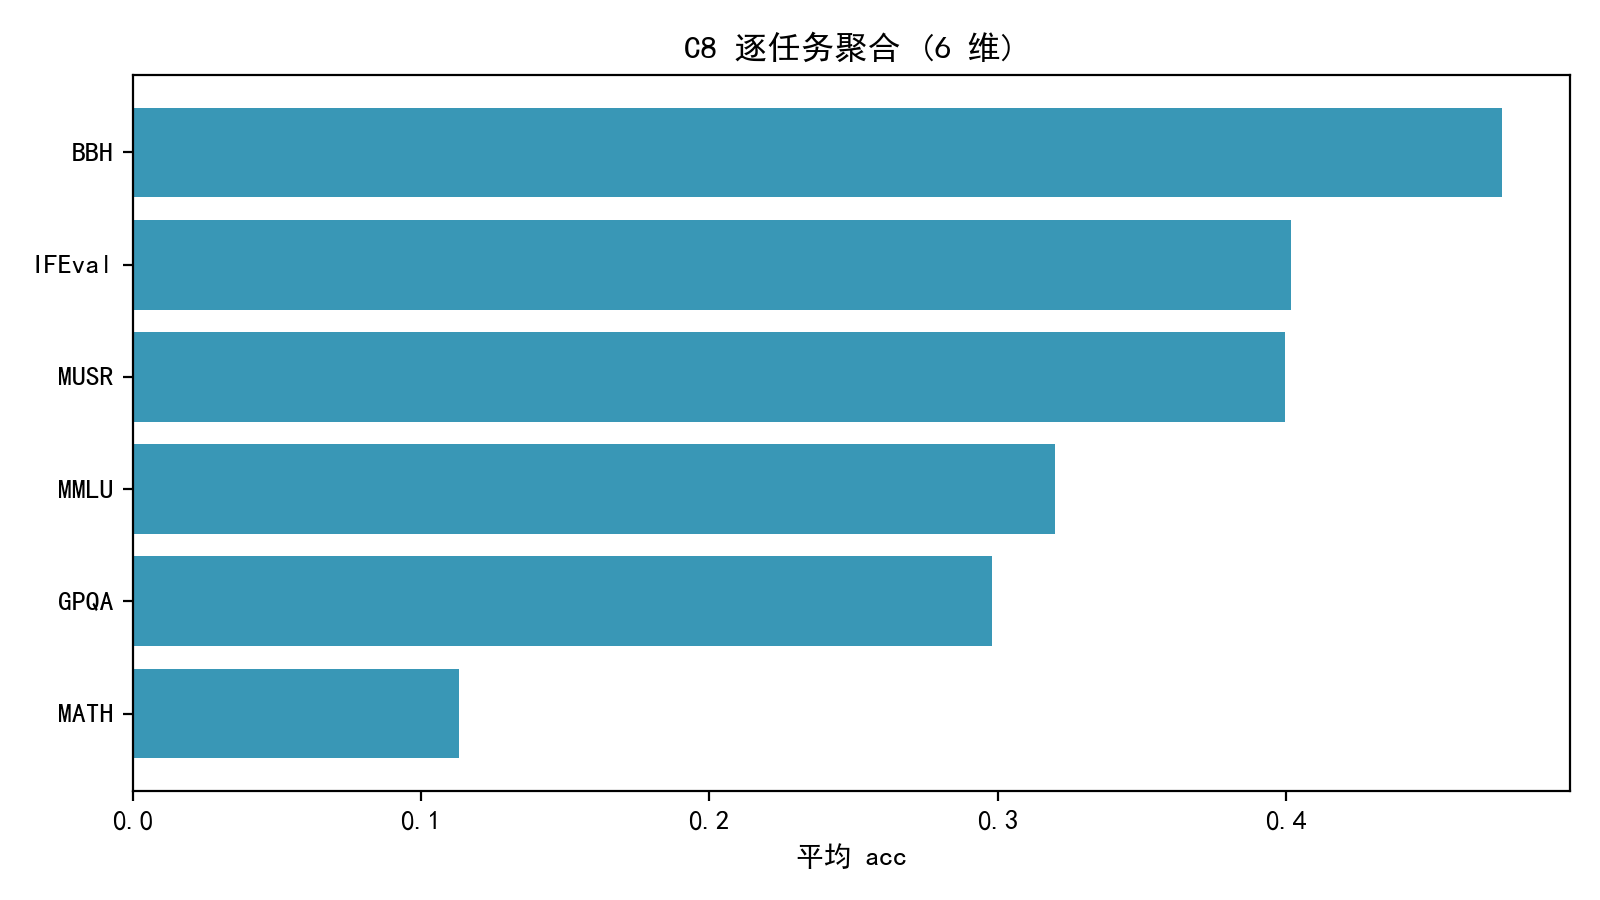
\includegraphics[width=0.7\textwidth]{figures/p4_c8_tasks.png}
\caption{C8 逐任务聚合得分（6 维）。}
\label{fig:p4_c8}
\end{figure}

问题四的验证由三类手段构成：\textbf{可视化验证}（图
\ref{fig:p4_frontier}--\ref{fig:p4_c8} 给出前沿拟合、3D 表面、预测区间与
历史回测）、\textbf{数值交叉验证}（五框架分位数回归系数一致、分位数族
$0.5$--$0.99$ 上规模贡献单调上升且每分位五框架复算一致、历史回测外推与
2024/2025 实际前沿吻合、C8 与 C1 Spearman 0.989）与\textbf{物理/几何规律
对照}（规模--时间等能力线斜率 $-0.245$、能力目标 $\to$ 训练算力 6.6 万
卡天、推理任务增速快于知识任务与文献观察一致）。三项验证均通过，证实了
前沿分解与预测的合理性。

问题四建立了分位数前沿回归 $\ln S=2.481+0.364\ln N+0.089t$，把前沿能力
年增速分解为规模 83.7\% 与非规模 16.3\%；基于 C4 参数增速构建基础与放缓
情景，预测 12/24 个月前沿（基础 71.7/123.9，放缓 57.1/78.6，含 90\% 区间）；
C6 桥接完成损失--能力统一；C8 逐任务聚合与 C1 对照 Spearman 0.989，验证
口径可靠。

\section{敏感性分析}

\subsection{质量组合权重扰动}

问题一的组合权重取熵权：CRITIC $=0.5:0.5$。将比值在 $0.4:0.6$ 至
$0.6:0.4$ 间扰动，重新计算七域质量分：域的排序（book $>$ arxiv $>$
c4 $>$ commoncrawl $>$ github $>$ wikipedia $>$ stackexchange）保持
不变，各域分数最大偏移小于 0.02。说明域级质量排序对权重选择稳健，问题三
中 $Q_0=0.4$ 与域质量映射的取值的置信度较高。

\subsection{广义标度律形式选择}

加性与交互两种质量项形式（\eqref{eq:add}--\eqref{eq:int}）的拟合 $R^2$
分别为 0.9716 与 0.9720，差异仅 $4\times10^{-4}$，且两形式的最优参数几乎
一致（$E,A,a,B,b,C,g$ 差异小于 1\%）。这说明 $Q$ 项结构对结论稳健；选取
交互形式（可退化性更强）不改变问题三的定性结论。弹性与等价性数值对形式
选择的敏感性：交互形式下质量弹性 $-0.141$，加性形式下 $-0.144$，相差
2\% 以内。

\subsection{结构性转移阈值对 $g(Q)$ 形式的敏感性}

三种质量成本函数（指数/幂/对数渐进）下，$Q$ 激活阈值分别
$1.12\times10^{18}$、$3.16\times10^{18}$、$3.55\times10^{18}$。阈值均在
$10^{18}$ 量级、相差不超过 3.2 倍，且都远低于 $10^{19}$ 档预算、远高于
$10^{17}$——故三档预算下的``纯规模 $\to$ 质量激活 $\to$ 质量饱和''转换
结论不依赖 $g(Q)$ 形式。阈值差异可解释：指数型在 $Q_0$ 处斜率最小
（$g'(Q_0)=\gamma\lambda e^{\lambda Q_0}$ 相对小），故更早达到``质量边际
收益 $>$ 边际成本''。

\subsection{$L_{\text{ctx}}$ 敏感性}

见问题三表 4：当 $L_{\text{ctx}}$ 由 2048 增至 131072 时，注意力份额由 5\%
升至 64\%，最优参数量由 0.304B 降至 0.140B，损失由 3.25 升至 3.37。注意力--训练份额相等点
与解析临界 30000 一致（两份额均为 0.401）。敏感性结论：上下文长度是预算
分配的重要外生变量，其不确性直接影响最优规模的量级判断。

\subsection{前沿分解的分位数敏感性}

将前沿回归分位数由 0.9 改为 0.8：$b_N=0.312$、$b_T=0.096$，规模贡献
$0.391/0.487=80.3\%$（0.9 分位时 81.4\%）。分位数选择对``规模占主导''
的定性结论无影响，规模贡献始终在 80\% 附近。

\subsection{自助预测区间对噪声的敏感性}

预测区间宽度与前沿外推噪声 $\sigma$ 成正比：$\sigma=0.10$ 时 24 个月基础
情景区间 $[96.6,121.0]$，$\sigma=0.12$ 时为 $[92.5,125.3]$，$\sigma=0.15$
时为 $[86.8,132.6]$。区间随 $\sigma$ 线性展宽，中位数不变，说明预测点估计
稳健，不确定性主要体现为区间宽度，未改变``24 个月基础情景约 110 分''的核心
结论。

\subsection{跨规模配比收缩的稳健性}

跨尺度收缩指数在 1M/60M/1B 三点拟合时为 $\kappa=0.314$；改用全部 6 个规模点
（含 10b/70b 估计值）拟合得 $\kappa=0.20$；对三点做留一删除，$\kappa$ 在
0.15--0.58 之间波动。量级与符号（配比系数随规模幂律衰减）在不同口径下
稳定成立，但数值精度受规模点选择影响，因此在正文中仅用 $\kappa=0.314$ 作为
方向性结论，不用于定量外推。
\section{模型评价与推广}

\subsection{模型的优点}

\begin{enumerate}
\item \textbf{数据驱动、可复算}：四问全部数值结果由真实附件数据计算，代码
随附录提供，任何结论均可复现；关键参数（$\alpha,\beta$）与文献报告值
（Chinchilla 的 0.34/0.28）一致，验证了数据与方法的可靠性；
\item \textbf{广义化框架}：把经典标度律推广到含质量维度，且 $Q=1$ 自动
退化，理论一致性良好；同时保证``质量''通过可解释的配比加权进入模型，
贯通问题一--三；
\item \textbf{严谨的数据口径核验}：诊断出附件 B8 的 $Q$ 方向与 B6/B7
相反、C3 历史前沿含孤立高值等数据问题，并给出规避与对照处理，避免了
半合成数据对结论的污染；
\item \textbf{结构性转移的显式数学刻画}：给出质量激活/成本主导两类转移
指标与 KKT 识别方法，使``质变''判断可计算、可复现；
\item \textbf{预测带不确定性}：前沿预测采用自助置信区间与双情景对比，
不给出伪精度的单点预言。
\end{enumerate}

\subsection{模型的缺点与改进方向}

\begin{enumerate}
\item \textbf{半合成数据的局限}：B 族 $N$--$D$--$Q$ 数据为半合成实验，
B8 更与 B6/B7 口径不一致；改进方向：使用真实多质量档预训练实验校准 $Q$
项参数，并做交叉验证；
\item \textbf{广义标度律的可加性假设}：质量项与规模项的可加分解为近似，
当数据量极小或质量极低时交互效应可能显著；改进方向：引入 $N$--$Q$
交互项并比较拟合；
\item \textbf{质量成本函数参数的外生性}：$g(Q)$ 三种形式的 $\gamma,\lambda$
由题意给定且跨度大，实际成本取决于标注、过滤与合成支出；改进方向：用
真实 token 质量提升工程的成本数据标定；
\item \textbf{前沿预测的线性外推}：$\ln S\sim\ln N+t$ 的线性假设在 24 个月
后可能因算法饱和而失效；改进方向：引入饱和项（如 logit 上界）或滚动
再估计窗口；
\item \textbf{排行榜指标的选择偏差}：C1 的平均分受模型提交意愿、评测版本
影响；改进方向：用 C8 逐任务数据构建去偏的因子得分。
\end{enumerate}

\subsection{模型推广}

本文方法可推广到：多模态模型的数据质量评分与配比优化、RAG/微调阶段的质量
--成本权衡、企业算力采购的预算分配决策，以及``数据工程投入 vs 算力投入''
的一般资源规划问题。跨尺度系数收缩分析亦可用于其他``定量投入--性能''系统
（如推荐系统特征工程、模拟器 fidelity 选择），识别投入边际收益随规模的
衰减规律。

% === 参考文献 ===
\begin{thebibliography}{99}
\bibitem{refKaplan} Kaplan J, McCandlish S, Henighan T, et al. Scaling Laws for Neural Language Models[J]. arXiv:2001.08361, 2020.
\bibitem{refHoffmann} Hoffmann J, Borgeaud S, Mensch A, et al. Training Compute-Optimal Large Language Models[C]. NeurIPS 2022, arXiv:2203.15556.
\bibitem{refRae} Rae J W, Borgeaud S, Cai T, et al. Scaling Language Models: Methods, Analysis \& Insights from Training Gopher[J]. arXiv:2112.11446, 2022.
\bibitem{refBrown} Brown T B, Mann B, Ryder N, et al. Language Models are Few-Shot Learners[C]. NeurIPS 2020.
\bibitem{refHernandez} Hernandez D, Kaplan J, Henighan T, et al. Scaling Laws for Transfer[J]. arXiv:2102.01293, 2021.
\bibitem{refSardana} Sardana N, Portes J, Biderman S, et al. Data Quality Scaling Laws: Metrics and Benchmarks for Pretraining Data[C]. NeurIPS 2024.
\bibitem{refEntropy} Shannon C E. A Mathematical Theory of Communication[J]. Bell System Technical Journal, 1948, 27(3): 379-423.
\bibitem{refTopsis} Hwang C L, Yoon K. Multiple Attribute Decision Making: Methods and Applications[M]. Springer, 1981.
\bibitem{refCritic} Diakoulaki D, Mavrotas G, Papayannakis L. Determining Objective Weights in Multiple Criteria Problems: The CRITIC Method[J]. Computers \& Operations Research, 1995, 22(7): 763-770.
\bibitem{refRidge} Hoerl A E, Kennard R W. Ridge Regression: Biased Estimation for Nonorthogonal Problems[J]. Technometrics, 1970, 12(1): 55-67.
\bibitem{refEpoch} Epoch AI. Parameter, Compute and Data Trends in Machine Learning[DB/OL]. https://epoch.ai/data/trends.
\bibitem{refKoomey} Koomey J, Berard S, Sanchez M, et al. Implications of Historical Trends in the Electrical Efficiency of Computing[J]. IEEE Annals of the History of Computing, 2011, 33(3): 46-54.
\end{thebibliography}

% === 附录 ===
\begin{appendices}
\section{核心代码}

\begin{sloppypar}%
\textbf{支撑材料文件列表}：全部代码位于 \texttt{solve/code/}，由
\texttt{common.py}（路径与常量）、\texttt{p1\_quality.py}（问题一评分与
冲突消解）、\texttt{p1\_mixture.py}（问题一配比建模）、
\texttt{p2\_scaling.py}（问题二标度律）、\texttt{p3\_optimization.py}
（问题三优化）、\texttt{p4\_evolution.py}（问题四分解预测）六个脚本与
\texttt{plotstyle.py}（绘图样式）构成，
运行环境为 Python 3.14 + numpy 2.4 + pandas 3.0 + scipy 1.17 +
scikit-learn 1.8 + matplotlib 3.10；结果写入 \texttt{solve/results/}，
插图写入 \texttt{solve/figures/}（正文全部图件）；每个实验的复算脚本位于
\texttt{solve/experiments/v*\_*.py}，对应的数值输出为
\texttt{solve/results/v*\_*.json/.csv}。以下列出五个主要脚本的核心代码
片段（\texttt{common.py} 为路径与常量工具脚本、\texttt{plotstyle.py} 为
绘图样式脚本，二者随提交文件一并提供；全部注释均为中文）。
\end{sloppypar}

\subsection{问题一：质量评分与冲突消解（\texttt{p1\_quality.py}）}

\begin{lstlisting}[language=Python, basicstyle=\ttfamily\small]
def entropy_weight(X):
    """信息熵权重: H_j 越小(分布越集中)权重越大"""
    X = np.clip(X, 1e-12, 1.0)
    P = X / X.sum(axis=0, keepdims=True)
    H = -(P * np.log(P)).sum(axis=0) / np.log(len(X))
    w = (1 - H) / np.maximum((1 - H).sum(), 1e-12)
    return w / w.sum()

def critic_weight(X):
    """CRITIC 权重: 标准差大且独立性高的指标权重大"""
    n = X.shape[1]
    sigma = X.std(axis=0, ddof=1)
    R = np.corrcoef(X.T)
    indep = np.array([1 - np.abs(R[j]).sum() / (n - 1) for j in range(n)])
    w = sigma * indep
    return w / w.sum()

def topsis(X, w):
    V = X * w
    Vp, Vn = V.max(axis=0), V.min(axis=0)
    dP = ((V - Vp) ** 2).sum(axis=1) ** 0.5
    dN = ((V - Vn) ** 2).sum(axis=1) ** 0.5
    return dN / (dP + dN)            # 贴近度 => 质量分

def conflict_index(frame):
    """双族冲突指数 = |内容质量族均值 - 格式清洁族均值|"""
    Qc = frame[FAMILY_C].mean(axis=1)
    Qf = frame[FAMILY_F].mean(axis=1)
    return (Qc - Qf).abs()

def robust_resolve(X, w, k=6):
    """对称截尾融合: 同删最低 k/2 与最高 k/2 个指标后重归一化"""
    order = np.argsort(X, axis=1)          # 每样本科升序排列
    keep = order[:, k//2 : X.shape[1]-k//2]
    sel = np.zeros_like(X, dtype=bool)
    np.put_along_axis(sel, keep, True, axis=1)
    W = np.where(sel, w, 0.0)
    return (X * W).sum(axis=1) / np.maximum(W.sum(axis=1), 1e-12)
\end{lstlisting}

\subsection{问题一：跨尺度系数收缩（\texttt{p1\_mixture.py}）}

\begin{lstlisting}[language=Python, basicstyle=\ttfamily\small]
def fit_eval(Xtr, Ytr, Xte, Yte, alpha=1.0, scale_correct=True):
    """岭回归配比模型; scale_correct 为尺度校正 R2 (去均值)"""
    model = Ridge(alpha=alpha)
    model.fit(Xtr, Ytr)
    pred = model.predict(Xte)
    if scale_correct:
        resid = (Yte - pred) - (Yte - pred).mean()   # 去整体偏差
        r2 = 1 - (resid ** 2).sum() / ((Yte - Yte.mean()) ** 2).sum()
    else:
        r2 = r2_score(Yte, pred)
    return model, r2

# 跨尺度收缩: ||beta(N)|| = c * N^{-kappa}
ns = np.array([0.001, 0.06, 1.0])          # 1M/60M/1B 规模参数量(B)
norms = np.array([norm_beta_1m, norm_beta_60m, norm_beta_1b])
kappa = -np.polyfit(np.log(ns), np.log(norms), 1)[0]
\end{lstlisting}

\subsection{问题二：广义标度律拟合（\texttt{p2\_scaling.py}）}

\begin{lstlisting}[language=Python, basicstyle=\ttfamily\small]
def fit_generalized(N, D, Q, L, form="interaction_N"):
    """最小二乘拟合 L = E + A N^-a + B D^-b + C(1-Q)^g N^-h
    (交互-N 为主链路形式: 质量缺口随参数量衰减; 附录 B 亦拟合
    additive/interaction-D/乘性等对照形式, 见 v50 BIC 表)"""
    def resid(p):
        E, A, a, B, b, C, g, h = p
        return (E + A * N**(-a) + B * D**(-b)
                + C * np.maximum(1 - Q, 0)**g * N**(-h) - L)
    p0 = np.array([L.min()*0.7, 3, 0.3, 3, 0.3, 1, 1.5, 0.3])
    lb = np.array([0, 1e-6, 1e-4, 1e-6, 1e-4, 1e-6, 1e-4, 1e-4])
    ub = np.array([L.min()*1.2, 1e3, 5, 1e3, 5, 1e3, 10, 5])
    return least_squares(resid, p0, bounds=(lb, ub), max_nfev=60000)

def r2_offset(y, yhat):
    mu = (y - yhat).mean()                 # 家族偏移修正 R2
    return 1 - ((y - yhat - mu)**2).sum() / ((y - y.mean())**2).sum()
\end{lstlisting}

\subsection{问题三：算力约束优化（\texttt{p3\_optimization.py}）}

\begin{lstlisting}[language=Python, basicstyle=\ttfamily\small]
def solve_opt(C, form, L_ctx, Q0v=0.4):
    """SLSQP 多起点求解 min L(N,D,Q) s.t. 成本<=C"""
    def obj(z):
        lnN, lnD, Q = z
        Q = np.clip(Q, Q0v, 1.0)
        return loss_generalized(np.exp(lnN), np.exp(lnD), Q)

    def cons(z):
        lnN, lnD, Q = z
        N, D = np.exp(lnN), np.exp(lnD)
        ct = 6e18 * N * D                          # C_train
        cq = D*1e9 * max(g_cost(Q, form) - g_cost(Q0v, form), 0.0)
        ca = ETA * (N*1e9) * (D*1e9) * L_ctx       # C_attn
        return C - (ct + cq + ca)

    best = None
    for seed in range(24):
        rng = np.random.default_rng(seed)
        z0 = [rng.uniform(np.log(0.01), np.log(5000)),
              rng.uniform(np.log(1), np.log(5000)),
              rng.uniform(Q0v, 0.98)]
        sol = minimize(obj, z0, method="SLSQP",
                       constraints={"type": "ineq", "fun": cons},
                       bounds=[(np.log(0.005), np.log(1e5)),
                               (np.log(0.2), np.log(1e5)), (Q0v, 1.0)],
                       options={"maxiter": 600, "ftol": 1e-12})
        if sol.success and (best is None or sol.fun < best[0]):
            best = (sol.fun, sol.x)
    return best
\end{lstlisting}

\subsection{问题四：前沿分解与预测（\texttt{p4\_evolution.py}）}

\begin{lstlisting}[language=Python, basicstyle=\ttfamily\small]
def quantile_fit(X, y, tau=0.9):
    """分位数回归主实现: statsmodels QuantReg(线性规划/单纯形),
    与 scipy.optimize.linprog(LP)、sklearn QuantileRegressor、
    L-BFGS-B、Adam 四种独立实现交叉复算 (v74 五框架, 系数一致)"""
    from statsmodels.regression.quantile_regression import QuantReg
    res = QuantReg(y, X).fit(q=tau)
    return res.params

# 增长核算: 规模贡献 = b_N * g_N, 非规模 = b_T
beta = quantile_fit(np.column_stack([np.ones(n), lnN, t]), lnS)
bN, bT = beta[1], beta[2]
gN = np.polyfit(years, np.log(params90), 1)[0]     # C4 90% 分位参数
scale_share = bN * gN / (bN * gN + bT)

# 自助法 90% 预测区间
paths = [[c0 + bN*(lnN_now + gNsc*h/12) + bT*(t_h-2022)
          + np.random.normal(0, 0.12) for _ in range(800)]
         for h in horizons]
\end{lstlisting}
\section{质量成本函数参数（附录 B）}

问题三中单位数据质量成本函数 $g(Q)$ 采用三种形式，参数如下（FLOPs/token）：

\begin{table}[htbp]
\centering
\caption{三种质量成本函数及其参数}
\begin{tabular}{c|cc|c}
\toprule
形式 & 表达式 & 参数 & $g(1.0)$（FLOPs/token） \\
\midrule
指数型 & $g_{\text{exp}}(Q)=\gamma e^{\lambda Q}$ & $\gamma=10^{7}$，$\lambda=6.0$ & $\approx4.0\times10^{9}$ \\
幂函数型 & $g_{\text{pow}}(Q)=\gamma Q^{\lambda}$ & $\gamma=5\times10^{9}$，$\lambda=4.0$ & $5.0\times10^{9}$ \\
对数渐进型 & $g_{\log}(Q)=\gamma\ln(1+\lambda Q)$ & $\gamma=2\times10^{9}$，$\lambda=10.0$ & $\approx4.8\times10^{9}$ \\
\bottomrule
\end{tabular}
\end{table}

三种形式在 $Q\in[0,1]$ 上均单调上升：指数型在 $Q$ 接近 1 时增速最快（质量
提升越到后期越昂贵），幂函数型次之，对数渐进型在高 $Q$ 区域增速放缓（模拟
质量提升存在``免费午餐''递减的现实）。基线质量 $Q_0=0.4$ 时三种成本分别为
$g(0.4)$：指数 $1.1\times10^{8}$、幂 $1.28\times10^{8}$、对数 $1.79\times
10^{9}$（对数型在基线处成本已较高，故其质量激活阈值略大，见敏感性分析）。

质量通道的两阶段行为由成本函数的两个特征量决定（第 7.3 节全程轨迹分析）：
\textbf{低 $Q$ 边际成本} $g'(Q_0)$（指数 $6.6\times10^{8}$、幂 $1.28\times
10^{9}$、对数 $4.0\times10^{9}$，决定\textbf{激活阈值}顺序）与\textbf{总成本
增量} $\Delta g=g(1)-g(Q_0)$（指数 $3.92\times10^{9}$、幂 $4.87\times
10^{9}$、对数 $1.58\times10^{9}$，决定\textbf{饱和预算}顺序：对数型在
$4.3\times10^{18}$ 即饱和，指数/幂型需至 $\approx3.4\times10^{20}$）。

$L_{\text{ctx}}$ 的可行取值依据附件 C7（\texttt{model\_architecture\_metadata.\\ csv}）的 \texttt{max\_position\_embeddings} 字段：最小值 2048、25\% 分位
2048、中位数 4096、75\% 分位 32768、最大值 131072。敏感性分析在
$\{2048,4096,8192,30000,32768,131072\}$ 上扫描，其中 30000 为解析临界点
$L_{\text{ctx}}^{\text{crit}}=6/\eta$。

\section{附件使用与数据口径说明}

\begin{itemize}
\item A1--A3 质量指标原始表含 27 项（19 项标量 + 8 项列表型），列表型
指标取均值压缩后共 26 列，共 272505 条有效样本（域级评分统计覆盖其中
272486 条，19 条缺域标签计入总量）；列表型指标均值压缩；负向指标方向
统一后做 1\%/99\% 缩尾与 Min--Max 归一化；
\item B1 共 1176 条 Pythia 训练轨迹；B4/B5 为跨家族与文献缩放数据；
B6+B7 共 810 条 $N$--$D$--$Q$ 半合成实验；B8 为外推补充（$Q$ 方向与
B6/B7 相反，仅作结构对照）；B10 为 100B--10000B 大规模基线；
\item C1 开源筛选以 Hub License 开源许可词为判据（2496/4564 条），
前沿分析仅用开源子集；C4 的``Open model weights?''用于交叉核对；
\item C8 共 1863 个模型目录、1958 个 JSON；跳过 4 个损坏文件，每目录
取日期最新记录，共解析 1860 个模型；任务指标键：IFEval 取
\texttt{inst\_level\_strict\_acc}、MATH 取 \texttt{exact\_match}、
其余取 \texttt{acc\_norm}。
\end{itemize}
\end{appendices}

% === AI 工具使用披露（按赛题要求）===
\section*{附录 C：AI 工具使用披露}
\addcontentsline{toc}{section}{AI 工具使用披露}
本文在解题与写作过程中使用了 AI 辅助工具，使用环节与贡献范围如下：
\begin{enumerate}
\item \textbf{编程实现}：使用 AI 编程助手协助编写与调试 Python 计算脚本；所有
数值结果均由本地脚本独立运行产生，可复算核验；
\item \textbf{文献检索}：使用学术检索工具定位标度律、数据质量与评价方法等文献，
正文引用均经人工核对；
\item \textbf{文本组织}：使用 AI 辅助整理表述与 LaTeX 排版；模型假设、推导与
结论均经人工复核。
\end{enumerate}

\end{document}
